\documentclass{article}
\usepackage[utf8]{inputenc} 
\usepackage[T1]{fontenc}   
\usepackage{lmodern}
\usepackage{hyperref}
\usepackage{graphicx} % Required for inserting images
\usepackage{subcaption}
\usepackage{blindtext}
\usepackage{titlesec}
\usepackage{amsthm}
\usepackage{amsmath}
\usepackage{standalone}
\usepackage[noabbrev]{cleveref}
\usepackage{float}
\usepackage{pgfplots}
\usepackage[labelsep=period]{caption}
\usepgfplotslibrary{fillbetween}
\usepackage[american]{circuitikz}

% Questa riga è  raccomandata per la compatibilità:
\pgfplotsset{compat=1.18}

\usepackage{amssymb}     % Necessario per \mathbb{C}
\usepackage{xcolor}      % Necessario per i colori (magenta, red)
\usepackage{tikz}        % Il pacchetto principale per disegnare
\usetikzlibrary{
	positioning,    % Per posizionare i nodi (es. below=of)
	arrows.meta,    % Per stili di freccia moderni (es. Stealth)
	calc,            % Per calcolare le coordinate (per la X)
	angles,          % Per l'angolo retto
	quotes,          % Per le etichette sugli angoli
	decorations.pathmorphing, % Per la freccia a "serpente"
	patterns,		% per il tratteggio
	decorations.pathreplacing
}

\graphicspath{{immagini/}}

\newtheorem{dfn}{Definizione}
\newtheorem{legge}{Legge}
\newtheorem{thr}{Teorema}
\newtheorem{proprietà}{Proprietà}
\newtheorem{es}{Esempio}
\newtheorem{ex}{Esercizio}
\renewcommand{\figurename}{Figura}
\crefname{figure}{Figura}{figure}
\crefname{ex}{Esercizio}{Esercizi}
\crefname{dfn}{Definizione}{Definizioni}
\crefname{equation}{Equazione}{Equazioni}



\title{Appunti del corso Sistemi e circuiti elettrici lineari}
\author{Docente del corso: dott. Arturo Popoli, PhD\\Appunti di: Lorenzo Murace}
\date{Primo Semestre a.a. 2025/2026}


\begin{document}

\maketitle
\pagebreak
\tableofcontents
\pagebreak

\include{cenniElettromagnetismo.tex}
\section{Elettromagnetismo nella materia}
\subsection{Polarizzazione elettrica}
La capacità di un campo elettrico di influenzare la materia viene detto \textsl{polarizzazione elettrica}.\\
Ci limitiamo, in questa sezione, alla trattazione del comportamento di materiali dielettrici, ossia materiali la cui conducibilità elettrica $\sigma\sim 10^{-6}\div10^{-7} S/m$ (Siemens/metro).
\begin{legge}[Legge di Ohm locale]
\begin{equation}\tag{Legge di Ohm locale}\begin{split}
\vec J = \sigma \vec E \\
\vec E = \rho \vec J
\end{split}
\end{equation}
$\sigma$ conducibilità elettrica.\\
$\rho = \frac{1}{\sigma}$ resistività elettrica.
\end{legge}

Sostanze dielettriche:
\begin{itemize}
\item Materiali apolari: \textsl{polarizzazione per deformazione}  A riposo, hanno un centro positivo e un esterno negativo, con baricentri positivo e negativo sovrapposti. Quando sottoposti a un campo elettrico, si deformano, e i due baricentri vengono spinti in due direzioni opposte, separandosi: si ottiene un sistema con una carica $+q$ e $-q$ a una distanza $d$, ossia un dipolo elettrico elementare, con momento di dipolo $\vec p = q\vec d$. Questa separazione porta alla generazione di un ulteriore campo, che interagisce con quello applicato, modificando il campo risultante percepito.
\item Materiali Polari: \textsl{polarizzazione per orientamento}. Esempio: acqua (distillata). Anche in assenza di $\vec E$ esterno, i baricentri delle cariche positive e negative non corrispondono, ed è dunque già un dipolo elettrico elementare, con $vec p = q \cdot \vec d$. All'applicazione di un campo esterno $vec E$, la carica positiva percepisce una forza concorde con il campo elettrico e quella negativa una discorde: si genera un momento torcente che porta all'allineamento del momento di dipolo al campo esterno e il campo generato dalla molecola si addiziona a quello esterno. Il forno a microonde ad esempio funziona sfruttando questo meccanismo: il campo elettrico variabile fa muovere le molecole d'acqua, e gli alimenti si scaldano per la dissipazione di energia tramite calore a livello molecolare.
\end{itemize}

Difficile descrivere il fenomeno a livello microscopico in una forma utile ed esaustiva, perciò lo facciamo a livello macroscopico, tramite una funzione continua nello spazio, che vale per entrambe le tipologie. Determiniamo un punto $\vec X$ e un volume infinitesimo che lo circonda $V$. $V$ contiene diversi dipoli: ne consideriamo una distribuzione casuale. Definiamo: $\Delta \vec p = \sum_{i \in V} \vec p_i$. Vettore polarizzazione elettrica $\vec P(\vec x) = \lim_{\Delta V \to 0} \frac{\Delta \vec p}{\Delta V}$, con le dimensioni $\frac{C}{m^2}$: è un momento di dipolo elettrico per unità di volume.\\
Si può dimostrare che $\nabla \cdot \vec P = - \rho_p$ con $\rho_p$ detta \textsl{densità di carica di polarizzazione}. Si può dunque descrivere il fenomeno come se fosse presente una densità di carica (di polarizzazione) dentro il materiale, la quale genera un campo.\\
Nel vuoto: 
\[\nabla \cdot \vec E = \frac{\rho}{\varepsilon_0}\]
Nella materia:
\[\nabla \cdot \vec E =\frac{\rho + \rho_p}{\varepsilon_0}\]
$\rho_p$ è difficile da rilevare: è necessario trovare un modo per esprimere questa relazione.\\
\[\nabla \cdot (\varepsilon_0 \vec E)=\rho - \nabla \cdot \vec P\]
\[\nabla \cdot (\varepsilon_0 \vec E + \vec P) = \rho\]
Definiamo il vettore \textsl{Campo di spostamento elettrico}.
\begin{dfn}[Campo di spostamento elettrico]
	\[\vec D = \varepsilon_0\vec E + \vec P\]
	Siccome $\vec P$ è funzione di $\vec E$, anche $\vec D$ lo è:
	\[\vec P = \vec P (\vec E) \Rightarrow \vec D = \vec D(\vec E)\]
\end{dfn}.\\
 Detto $\bar{\bar{\alpha}}$ \textsl{tensore di polarizzazione} (determinato sperimentalmente nell'ambito della fisica della materia),
\[\vec P = \bar{\bar{\alpha}} \vec E\]
Per un materiale non lineare, le entrate di $\bar{\bar{\alpha}}$ dipendono dal modulo delle componenti di $\vec E$. Per un materiale isotropo e lineare, invece, $\bar{\bar{\alpha}}$ si riduce a un multiplo, detto \textsl{suscettività elettrica} ($\chi_e$) della matrice identità. Dunque, per un materiale isotropo e lineare: 
\[\vec P = \varepsilon_0 \chi_e \vec E \]
\[\vec D = \varepsilon_0 \varepsilon_r \vec E \]
con $\varepsilon_r = 1 + \chi_e$, e ha valore $1$ nel vuoto $\sim 1$ nell'aria, $2 \div 5$ nei solidi isolanti e $\sim 80$ nei liquidi isolanti.\\
Ne risulta dunque che tutte le proprietà qualitative di $\vec E$ già studiate valgono anche per $\vec D$.

\subsection{Magnetizzazione}
Essendo il magnetismo un fenomeno quantistico a livello microscopico, le teorie che consideriamo vengono ancora utilizzate soltanto perché funzionanti a livello macroscopico, non perché sostanzialmente corrette. 

Si considera un'ipotetica traiettoria chiusa circolare di un elettrone in rotazione attorno a un nucleo come una spira percorsa da corrente, che racchiude una superficie. Tale spira costituisce un dipolo magnetico elementare, con momento di dipolo magnetico $\vec \mu = i \Delta \vec S \hat n = i \Delta \vec S$, misurato in $A\ m^2$.
Ci chiediamo dunque come reagisca un atomo o molecola così costituito se sottoposto a un campo di induzione magnetica.\\
$\vec B \neq 0$ orienta la spira portando la normale ad esservi parallela. Attuiamo una descrizione macroscopica analoga a quella impiegata per la polarizzazione elettrica per allineamento. $\Delta \vec m = \sum_{i \in V} m_i$ attorno a un punto $\vec X$. $\vec M (\vec X) = \lim_{\Delta V \to 0} \frac{\Delta m}{\Delta V}$: momento di dipolo magnetico per unità di volume, misurata in $A/m$.
Si può dimostrare che:
\[\nabla \times \vec M = \vec J_m\] con $\vec J_m$ \textsl{densità di corrente di magnetizzazione}.
\[ \frac{\partial \vec P}{\partial t} = \vec J_p \] con $\vec J_p$ \textsl{densità di corrente di polarizzazione}.\\
Nel vuoto: $\nabla \times (\frac{1}{\mu_0} \vec B) = \vec J + \frac{\partial \varepsilon_0 \vec E}{\partial t}$.\\
Nella materia: $\nabla \times (\frac{1)}{\mu_0} \vec B) = \vec J + \vec J_m \frac{\partial \varepsilon_0 \vec E}{\partial t} + \frac{\partial \vec J_p}{\partial t}$.
\[\nabla \times (\frac{1}{\mu_0} \vec B) = \vec J + \vec J_m \frac{\partial}{\partial t} \varepsilon_0 \vec E +\vec J_p\]
\[\nabla \times (\frac{1}{\mu_0} \vec B - \vec M) = \vec J + \frac{\partial \vec D}{\partial t}\]
Definiamo dunque il \textsl{campo magnetico} 
\begin{dfn}[Campo magnetico]
	\[\vec H = \frac{1}{\mu_0} \vec B - \vec M\ (A \cdot m^{-1})\]
	Per evitare ambiguità, si definisce $\vec B = \mu_0 (\vec H + \vec M)$ \textsl{campo di induzione magnetica}).
	Siccome $\vec M$ è funzione di $\vec H$, anche $\vec B$ lo è.
	\[\vec M = \vec M (\vec H) \Rightarrow \vec B = \vec B(\vec H)\]
\end{dfn}
Analogamente a quanto fatto per la descrizione del fenomeno della polarizzazione elettrica, si definisce un \textsl{tensore di magnetizzabilità}, che nel caso di materiali isotropi e lineari si porta alla relazione $\vec M = \chi_m \vec H$, con $\chi_m$ detto \textsl{suscettività magnetica}.
\[\nabla \times \vec H = \vec J + \frac{\partial \vec D}{\partial t}\]
In questo modo si è espresso $\vec H$ soltanto in funzione delle correnti libere e di polarizzazione elettrica, ma non di polarizzazione magnetica. Da qui, è poi possibile determinare $\vec B$. Per un materiale isotropo e lineare, $\vec B = \mu_0 \mu_r \vec H$, con $\mu_r = 1 + \chi_m$ \textsl{permeabilità magnetica relativa}. $\mu_r$ ha valori: $1$ nel vuoto, $\sim 1$ nell'aria, $<1$ nei materiali diamagnetici, $>1$ nei materiali paramagnetici e $\gg 1$ per materiali ferromagnetici.
\section{Ricapitolazione: Leggi dell'elettromagnetismo nella materia}
\begin{description}
%\begin{itemize}
	\item [1. Legge di Gauss per il campo di spostamento elettrico] \[\nabla \cdot \vec D = \rho \qquad \rightarrow \qquad \oint_S \vec D \cdot d\vec S = Q\]
	\item [2. Legge di Gauss per il campo magnetico]  \[\nabla \cdot \vec B = 0 \qquad \rightarrow \qquad \oint_S \vec B \cdot d\vec S = 0\]
	\item [3. Legge di Faraday] \[\nabla \times \vec E = -\frac{\partial \vec B}{\partial t} \qquad \rightarrow \qquad \oint_\Gamma \vec E \cdot d \vec l = -\frac{d}{dt}\Phi_{\vec B,\Gamma}\]
	\item [4. Legge di Ampère] \[\nabla \times \vec H = \vec J +\frac{\partial \vec D}{\partial t} \qquad \rightarrow \qquad \oint_\Gamma \vec H \cdot d \vec l = \Phi_{\vec J,S} + \Phi_{\frac{\partial \vec D}{\partial t},S} = i + i_s\]
	\item [5. Equazione di continuità] \[\frac{\partial \rho}{\partial t} + \nabla \cdot \vec J = 0 \qquad \rightarrow \qquad i = - \frac{dQ}{dt}\]
	\item [6. Relazioni di legame materiale] Per materiali isotropi e lineari:
	\begin{itemize}
		\item $\vec D = \varepsilon_0 \varepsilon_r \vec E$
		\item $\vec B = \mu_0 \mu_r \vec H$
		\item $ \vec J = \sigma (\vec E + \vec E_i)$ dove $\vec E_i$ sono i campi elettrici \textsl{impressi}, cioè di origine non elettrica.
	\end{itemize}
\end{description}
%\end{itemize}
\section{Introduzione ai circuiti elettrici a parametri concentrati}
\subsection{Definizioni fondamentali}
Si distinguerà d'ora in poi tra:
\begin{description}
	\item [\textsl{circuito fisico}]: ha luogo nella realtà ed è costituito da componenti materiali (es. un filo in cui circola corrente, la stessa per ogni sezione, in quanto è un tubo di flusso di $\vec J_t$). Risolverlo significa risolvere le equazioni di Maxwell nella materia che costituiscono un sistema di equazioni differenziali alle derivate parziali $f(x,y,z,t)$. Si ottiene come risultato una soluzione esatta, analitica per i valori di tutti i campi in ogni posizione nello spazio: problema $3D$ (tre coordinate spaziali e una temporale)
	\item[\textsl{circuito a parametri concentrati}]: Rappresentazione approssimata di un circuito fisico, mediante \textsl{componenti (circuitali)} e \textsl{collegamenti ideali}. Utile a una risoluzione approssimata ma comunque affidabile e più rapida del sistema. Rinunciando alla descrizione accurata (in termini di coordinate spaziali), risolvere il circuito significa risolvere un sistema di equazioni differenziali ordinarie: problema $0D$ (solo coordinata temporale).\\
	Si fonda su tre ipotesi:
	\begin{itemize}
		\item i collegamenti sono ideali ($\sigma = \infty\ \iff \rho = 0$)
		\item lo spazio esterno ai collegamenti e ai componenti è perfettamente isolante ($\sigma = 0\ \iff \rho = \infty$)
		\item nello spazio esterno, (1) $\frac{\partial \vec B}{\partial t}\approx 0$, cosicché $\vec E$ sia conservativo e $\vec E = \nabla \varphi$ dove $\phi$ è il potenziale elettrico, misurato in $V$ e (2) $\frac{\partial \vec D}{\partial t}\approx 0$, cosicché $\nabla \times \vec H = \vec J$ e dunque $\vec J$ è un campo solenoidale ($\nabla \cdot \vec J = 0$). Da queste due condizioni derivano le Leggi di Kirchhoff.
	\end{itemize}
\end{description}
\subsubsection{Parti del circuito}
\begin{dfn}[componente]
	Sottosistema delimitato da una \textsl{superficie limite} che può essere attraversata da correnti sono in corrispondenza dei \textsl{terminali}, ossia le regioni di contatto con i collegamenti esterni.\\
	Un componente con 2 terminali è detto \textsl{dipolo}; uno con 3, \textsl{tripolo}, uno con n, \textsl{n-polo}.
\end{dfn}
\begin{dfn}[Nodo (polo)] Un nodo (o polo) si intende indistintamente una delle due seguenti configurazioni:
	\begin{enumerate}
		\item terminale isolato
		\item insieme di più terminali connessi da collegamenti ideali.
	\end{enumerate}
\end{dfn}
\begin{dfn}[Ramo]
	Tratto del circuito che unisce due nodi adiacenti.
\end{dfn}
\begin{legge}[Principio di invarianza topologica]
	Osserviamo che alcuni fatti soltanto alcuni fatti sono rilevanti per il comportamento del circuito.
	\begin{description}
		\item[Influenzano il comportamento del circuito:] \leavevmode
		\begin{itemize}
			\item la tipologia dei componenti
			\item la topologia del circuito
		\end{itemize}
		\item[Non influenzano il comportamento del circuito:] \leavevmode
		\begin{itemize}
			\item la posizione dei componenti nello spazio (infatti la sua rappresentazione non corrisponde a posizioni spaziali nella realtà)
			\item la forma dei collegamenti (che infatti sono ideali)
		\end{itemize}
		
	\end{description}
\end{legge}
\begin{dfn}[Maglia]
	Percorso chiuso formato da rami del circuito che attraversa una sequenza chiusa di nodi, senza passare più di una volta per lo stesso nodo.
\end{dfn}
\subsubsection{Grandezze}
\begin{dfn}[Corrente]
	La consideriamo dovuta a un moto di cariche positive (+), per convenzione.\\
	\[i=\int_S \vec J \cdot d\vec S = \frac{dQ}{dt}\]
	con $S$ generica perché il circuito è un tubo di flusso per $J$ campo solenoidale (per le ipotesi sopra).\\ 
	Ne risulta che:
	\[\Delta Q = \int_t^{t+\Delta t} i(t)dt\]
	È necessario definire un \textsl{verso di riferimento (VDR)} per effettuare il calcolo di una corrente $i$ tra due punti, in analogia con la necessità di assegnare un verso alla normale della superficie per calcolare il flusso. Tale verso è (1) arbitrario e (2) costante nel tempo. Effettuati i calcoli, è possibile che il \textsl{verso effettivo} risulti concorde ($i>0$) oppure discorde ($i<0$) con quello di riferimento.
\end{dfn}
\begin{dfn}[Tensione]\label{dfn:tensione}
	Variazione di energia per unità di carica quando una carica puntiforme si sposta da un A a B.
	\[v_{AB}=\int_A^B \vec E \cdot d \vec l = - \int_A^B \nabla \varphi \cdot d \vec l = - (\varphi(B) - \varphi(A))= \varphi_A - \varphi_B\]
	Tensione e differenza di potenziale in generale non sono la stessa cosa. Coincidono soltanto nel caso in cui $\nabla \times \vec E = 0$, ossia se $\vec E$ è conservativo.\\
	Per calcolare la tensione tra due punti, è necessario determinare un verso di riferimento, arbitrario e costante. Se $v_{AB}>0$, una carica che si sposta da $A$ a $B$ perde energia potenziale elettrica. Viceversa, $v_{AB}<0$, una carica che si sposta da $A$ a $B$ perde energia.
\end{dfn}
\subsection{Leggi di Kirchhoff - Leggi topologiche}
\begin{legge}[Legge di Kirchhoff delle correnti - LKC]
	La somma algebrica delle correnti attraverso qualsiasi superficie $S$ chiusa esterna alle superfici limite dei componenti è nulla.\\
	Per esempio, si consideri una superficie che taglia tre rami e include un nodo ($S_1$ in \cref{fig:lkc}). Possibile considerare anche una superficie che include più nodi. Oppure ancora, una superficie che circondi sostanzialmente soltanto un nodo ($S_2$ in \cref{fig:lkc}): in questo caso prende il nome di \textsl{legge nodale}.
	\begin{figure}[h]
		\centering
		\includegraphics[width=0.8\linewidth]{LKC}
		\caption{}
		\label{fig:lkc}
	\end{figure}
\end{legge}

Indaghiamo il collegamento tra la LKC e la Teoria dei campi. Considero un circuito  e una superficie che circondi un nodo tra più rami. Risulta (considerando il riferimento di \cref{fig:lkc}, e indicando le superfici di sezione del filo con apici): \[\oint_{S_2} \vec J_t \cdot d \vec S = \oint_{S_2} \vec J \cdot d \vec S = \int_{S_2'} \vec J \cdot d\vec S + \int_{S_2''} \vec J \cdot d\vec - \int_{S_2'''} \vec J \cdot d\vec S = i_4 + i_5 - i_6.\] Dunque la LKC è una conseguenza del carattere solenoidale di $\vec J$ (fuori dalle superfici limite dei componenti).\\
Conseguenze della LKC:
\begin{description}
	\item[corrente di ramo]. Un bipolo in generale avrebbe una corrente entrante e una uscente distinte. Ma per la LKC la loro somma algebrica deve essere nulla, dunque devono essere uguali.
	\item [corrente in un ramo aperto (circuito aperto)]. La corrente in un ramo aperto può soltanto essere nulla, altrimenti si avrebbe una corrente entrante nel nodo terminale e nessuna corrente uscente.
\end{description}

\begin{legge}[Legge di Kirchhoff delle tensioni - LKT]
	La somma algebrica delle tensioni lungo una curva chiusa esterna $\Gamma$ alle superfici limite dei componenti passante per una sequenza di nodi è nulla.\\
	Per esempio, considerando la \cref{fig:lkt}, assegnato verso di riferimento a $\Gamma_1$ e alle tensioni tra i nodi. Un caso particolare si ottiene considerando la curva $\Gamma_2$, coincidente con una maglia del circuito.
	
	\begin{figure}[h]
		\centering
		\includegraphics[width=0.8\linewidth]{LKT}
		\caption{}
		\label{fig:lkt}
	\end{figure}
	
	
\end{legge}
Indaghiamo il collegamento tra la LKT e la Teoria dei campi.
 \[\oint_{\Gamma_1} \vec E \cdot d \vec l = -\frac{d}{dt} \Phi_{B,\Gamma_1} = 0 = \sum_i \int_{A_i}^{B_i} \vec E \cdot d\vec l = \sum_i v_{A_i B_i}\]
\subsection{Potenza ed energia}
\begin{dfn}[Potenza per un bipolo]
	Consideriamo un bipolo generico sottoposto a una generica $v(t)$, attraversato da una $i(t)$. Definiamo la potenza istantanea (assorbita o erogata dal componente) $p(t) = \frac{dW(t)}{dt} = \frac{dW(t)}{dQ} \frac{dQ}{dt} = v(t)i(t)$.\\
	In circuiti in regime stazionario (corrente continua), $p(t) = P$ è la potenza, costante nel tempo.
\end{dfn}
Convenzioni nei versi di riferimento (calcolo potenza): 
\begin{description}
	\item[convenzione dell'utilizzatore] VDR i entrante nel polo (+) (definito in base a $v$): cariche da (+) a (-), quindi perdono energia (potenziale). L'energia (potenza) viene assorbita (dissipata) dal componente, dunque detto \textsl{utilizzatore}. $vi = P_A$ Potenza assorbita (se negativa, il componente eroga energia).
	\item[convenzione del generatore] VDR i uscente dal polo (+): cariche da (-) a (+), quindi guadagnano energia. L'energia (potenza) viene erogata dal componente. $vi = P_E$ Potenza erogata (se negativa, il componente assorbe energia).
\end{description}
Enunciamo ora un teorema fondato sulla validità delle Leggi di Kirchhoff.
\begin{thr}[Teorema di conservazione della potenza istantanea]
	Per ogni circuito elettrico, la somma algebrica delle potenze erogate è uguale alla somma algebrica delle potenze istantanee assorbite.\\
	Se $n$ sono componenti eroganti e $m$ sono utilizzatori.
	\[\sum_{i=1}^{n} P_{E,i}(t) = \sum_{j=1}^{m} P_{A,j}(t)\]
	Nella L5 è proposto un esempio di verifica del teorema.
\end{thr}
Implicazioni del teorema di conservazione della potenza istantanea. Siccome è valido anche nei circuiti reali. Ne vediamo alcuni esempi per la rete elettrica nazionale. Su dati.terna.it è possibile trovare dati sul fabbisogno nazionale nel tempo. L'andamento del fabbisogno è molto vario nel tempo (giorni, ore, mesi). Le fonti sono varie perché è necessario avere una adeguata adattabilità al fabbisogno, e l'accumulo di energia non è facile ed esteso.  L'idroelettrico (programmabile) è ormai al massimo, perché gli specchi d'acqua sfruttabili sono quasi al limite. Con quelle rinnovabili non programmabili è difficile ottenere di più in maniera affidabile.\\
Confronto tra i profili di produzione francese (con molto nucleare) e italiano (con più rinnovabili ma anche più gas).\\
Mappa dei consumi come indice di produttività della regione\\
Interventi sulla rete elettrica al 2030 e 2034: molti collegamenti. Obiettivo: renderla più "magliata" per consentire continuità elettrica. L'Italia è avanzata come paese industriale proprio grazie all'affidabilità della rete elettrica.\\
Crisi elettrica in Texas nel Febbraio 2021. Il Texas, per pagare meno tasse federali non è connesso alla rete elettrica federale (esistono una rete Western e una Eastern, con poche connessioni perché in mezzo ci sono le Montagne Rocciose) (dunque ha una rete propria, connessa con Messico e altri, ma molto più fragile: per questo è molto più esposto). Vedi immagini di Houston prima e dopo gli eventi (wikipedia). Le elevate spese italiane per l'interconnessione interna e con altri paesi ha grandi importanza per l'affidabilità della rete.\\
Ipotizzato lo stoccaggio dell'energia, per aumentare la penetrazione delle fonti di energia non programmabili. Per piccole comunità elettriche può funzionare (UPS). Per potenze molto elevate, sopperire alla non-programmabilità con le attuali batterie non è possibile, per costi e disponibilità di materiali. Tra le direzioni di sperimentazione, superconduttori e riciclo di batterie dall'automotive. Si sente di alcuni paesi che ottengono l'80\% della loro energia dal fotovoltaico, ma si tratta sempre di paesi piccoli: impossibile per fabbisogni più elevati.\\
\\
\begin{dfn}[Energia assorbita ed erogata]
	\[W(t) = \int_t^{t+\Delta t} p(t) dt = \int_t^{t+\Delta t} v(t) i(t)dt \]
	Secondo la convenzione già illustrata per la potenza, si parla di energia assorbita $W_A$ ed energia erogata $W_E$.
	Se $p(t)=P$, $W(\Delta t) = P \Delta t$.\\
	Unità di misura comuni, oltre ai $J$, sono i $Wh$ e il suo multiplo $kWh$.
\end{dfn}

\subsection{Leggi costitutive - Introduzione e classificazione}
Mentre le leggi di Kirchhoff sono \textsl{leggi topologiche}, studiamo ora le leggi che caratterizzano il comportamento di particolari componenti del circuito: le \textsl{leggi costitutive}, nella forma $f(v(t), i(t))=0$.
Classificazione dei componenti:
\begin{description}
	\item [In base alla forma della legge costitutiva (LC)]\leavevmode
	\begin{description}
		\item[Senza memoria (anche detti resistivi, algebrici, adinamici)] LC algebrica. Es. $v(t)=\alpha i(t) + \gamma$.
		\item [Con memoria (dinamici)] LC integro-differenziale. Es. $v(t)= \varepsilon \int_{-\infty}^t i(t)dt$
	\end{description}
	\item [In base alla linearità] lineari o non lineari.\leavevmode
	\item [In base alla tempo-varianza]\leavevmode
	\begin{description}
		\item[Tempo-invarianti] La dipendenza temporale non è esplicita ($t$ compare soltanto come argomento di $v(t), i(t)$)
		\item[Tempo-varianti] La dipendenza temporale è esplicita. Tutti i componenti lo sono, ma alcuni si possono approssimare a tempo-invarianti.
	\end{description}
	\item [In base ad attività o passività: ]\leavevmode
	\begin{description}
		\item[Passivi:] $W_A (t) =\int_{-\infty}^t p_A(t) dt \geq 0 \quad \forall t$. Il componente può anche erogare energia, ciò che lo definisce è che l'energia totale assorbita sia sempre positiva (può erogare soltanto energia assorbita, non ne genera).
		\item[Attivi: ] $\exists t\ | \quad W_A (t) <0 $.
	\end{description}
	\item [In base alla potenza scambiata: ]\leavevmode
	\begin{description}
		\item [Dissipativi:] $p_A (t) \geq 0 \quad \forall t$
		\item [Inerti: ] $p_A(t) = 0 \quad \forall t$
	\end{description}
	\item [In base al tipo di controllo] \leavevmode
	\begin{description}
		\item[controllati in tensione] Nella LC, $v(t)$ è la variabile indipendente
		\item [controllati in corrente] Nella LC, $i(t)$ è la variabile indipendente.
	\end{description}
\end{description}
\subsection {Collegamenti di bipoli in serie e parallelo}
\begin{dfn}[Serie]
	(1) Due bipoli sono collegati in serie se condividono un nodo a cui non afferiscono altri rami. Si osserva che in una configurazione del genere, i componenti in serie sono attraversati dalla stessa corrente; pertanto si può dare una definizione più generale di "collegamento in serie" (la 2).
	(2)Due o più bipoli sono in serie se sono attraversati dalla stessa corrente.
\end{dfn}
\begin{dfn}[Parallelo]
	(1) Due o più bipoli sono collegati in parallelo se sono connessi alla stessa coppia di nodi. Si osserva che in una configurazione del genere, i componenti in parallelo sono sottoposti alla medesima tensione; pertanto si può dare un'ulteriore definizione di "collegamento in parallelo" (la 2).
	(2) Due o più bipoli sono in parallelo se sono sottoposti alla stessa tensione.
\end{dfn}
\section{Resistore lineare}
\begin{dfn}[Resistore lineare]
	Componente circuitale in cui si "concentra" la proprietà fisica della resistenza elettrica. È più che un semplice modello del resistore fisico, in quanto può assumere le proprietà di resistenza di altre parti del circuito. 
\end{dfn}
\begin{legge}[Legge costitutiva del resistore lineare] \[ v(t) = R i(t)\]
	\[i(t) = G v(t)\]
	secondo la convenzione dell'utilizzatore. $R$ è detta \textsl{resistenza elettrica} ed è misurato in $\Omega$ (\textsl{Ohm}); $G =\frac{1}{R}$ \textsl{conduttanza elettrica}, misurata in $S$ (Siemens)
\end{legge}
Classificazione del componente:
\begin{itemize}
	\item Controllato in corrente e in tensione;
	\item Lineare ($R$ non dipende da $i(t)$; $G$ non dipende da $v(t)$);
	\item Senza memoria;
	\item Tempo-invariante ($R$ è costante);
	\item Passivo ($p_A(t)= Ri^2(t) = G v^2(t) \geq 0 \Rightarrow W_A(t) \geq 0$;
\end{itemize}
\subsection{Resistori in serie e partitore di tensione}
Resistori in serie:
\[LKT_{\Gamma}: v= \sum_k v_k= (\sum_k R_k) i = R_{eq} i\]
con $R_{eq} = \sum_k R_k$. Posso dunque semplificare il circuito considerando la serie come un unico resistore con resistenza $R_{eq}$.
\begin{dfn}[Partitore di tensione]
	Serie di resistori. Ci interessiamo alla caduta di tensione dopo ciascun resistore.\\
	Detta $v$ la tensione applicata alla serie, la caduta di tensione sul resistore $k$-esimo è \[v_k = \frac{R_k}{R_{eq}}v\]
\end{dfn}
\subsection{Resistori in parallelo e partitore di corrente}
Resistori in parallelo:
\[LKC_A: i = \sum_k i_k = \sum_k G_kv = (\sum_k G_k) v = G_{eq} v\]
con $G_{eq} = \sum_k G_k = \frac{1}{R_{eq}}$, da cui $R_{eq} = \frac{1}{\sum_k \frac{1}{R_k}}$. Posso dunque semplificare il circuito considerando la serie come un unico resistore con resistenza $R_{eq}$.
\begin{dfn}[Partitore di corrente]
	Parallelo di resistori. Ci interessiamo alla corrente che scorre in ciascun resistore.\\
	Detta $i$ la corrente che scorre nel parallelo, la corrente che scorre nel resistore $k$-esimo è \[i_k = \frac{G_k}{G_{eq}}i = \frac{R_{eq}}{R_k} i \]
\end{dfn}
\subsection{Cortocircuito}
Nel caso in cui uno dei rami del parallelo abbia resistenza nulla, tutta la corrente passa in quel ramo, e la tensione ai due capi risulta nulla. Definiamo un ramo così caratterizzato \textsl{componente cortocircuito}.
\begin{dfn}[Componente cortocircuito]
	Tratto di conduttore ideale
\end{dfn}
\begin{legge} [Legge costitutiva del cortocircuito]
	\[v(t) = 0 \quad \forall i(t)\]
\end{legge}
Osserviamo che questo è un componente inerte ($p_A(t)= 0 \quad \forall i(t)$;
Un cortocircuito reale ha una resistenza molto piccola ma finita, dunque vi può circolare un'elevata corrente, che può essere dissipata in calore al punto da generare, ad esempio, incendi.

\subsection{Circuito aperto}
Simmetricamente, nel caso in cui un ramo abbia resistenza infinita, tutta la corrente passa nel ramo opposto, e tale si comporta come un circuito aperto. 
\begin{dfn}[Componente circuito aperto]
	Tratto con resistenza infinita.
\end{dfn}
\begin{legge} [Legge costitutiva del cortocircuito]
	\[i(t) = 0 \quad \forall v(t)\]
\end{legge}
Osserviamo che anche questo è un componente inerte ($p_A(t)= 0 \quad \forall v(t)$.

\subsection{Trasformazioni triangolo-stella nella connessione di resistori}
\begin{figure}[H]
	\centering
	\begin{subfigure}[b]{0.45\textwidth}
		\centering
		\includegraphics[width=\linewidth]{triang}
	\end{subfigure}
	\hfill
	\begin{subfigure}[b]{0.45\textwidth}
		\centering
		\includegraphics[width=\linewidth]{stella}
	\end{subfigure}
	\caption{Configurazioni di resistori a triangolo (a sinistra) e a stella (a destra).}
	\label{fig:triang_stella}
\end{figure}
Per ottenere la \textbf{\textsl{stella equivalente al triangolo}}:
\begin{itemize}
	\item [1] Aggiungere un centro-stella;
	\item [2] Disegnare $R_A$, $R_B$, $R_C$
	\item [3] Si dimostra che: 
	\begin{equation}\tag{trasformazioni triangolo-stella}
		\label{eq:triangolo-stella}
		\begin{split}
			R_A = \frac{R_{AB}R_{AC}}{R_{AB} + R_{BC} + R_{AC}}\\
			R_B = \frac{R_{AC}R_{BC}}{R_{AB} + R_{BC} + R_{AC}}\\
			R_A = \frac{R_{AB}R_{AC}}{R_{AB} + R_{BC} + R_{AC}}
		\end{split}
	\end{equation}
\end{itemize}
Nel caso particolare $R_{AB}=R_{BC}=R_{AC}= R_{\Delta}$, $R_A = R_B = R_C = R_{\Delta}/3$.\\
\\

Al contrario, per ottenere il \textbf{\textsl{triangolo equivalente alla stella}}:
\begin{itemize}
	\item [1] Rimuovere centro-stella;
	\item [2] Disegnare $R_{AB}$, $R_{BC}$, $R_{AC}$
	\item [3] Si dimostra che: 
	\begin{equation}\tag{trasformazioni stella-triangolo}
		\label{eq:stella-triangolo}
		\begin{split}
			R_{AB} = \frac{R_{A}R_{B} + R_{B}R_{C} + R_{A}R_{C}}{R_C}\\
			R_{BC} = \frac{R_{A}R_{B} + R_{B}R_{C} + R_{A}R_{C}}{R_A}\\
			R_{AC}=  \frac{R_{A}R_{B} + R_{B}R_{C} + R_{A}R_{C}}{R_B}
		\end{split}
	\end{equation}
\end{itemize}
Nel caso particolare $R_{A}=R_{B}=R_{C}= R_{stella}$, $R_{AB} = R_{BC} = R_{AC} = 3R_{stella}$.\\
\\
Per un esercizio sul tema, si faccia riferimento all'\cref{esercizio:3}. L'esercizio è riportato in seguito perché comprende un generatore, componente che sarà trattato nel prossimo capitolo. 


\section{Generatori indipendenti di tensione e di corrente}
\subsection{Generatori ideali}
\begin{dfn}[Generatore indipendente di tensione]
	Nella notazione U.S., il simbolo è un cerchio con un segno + e uno - che ne indicano la polarità. Chiamiamo $V_g$ la fem del generatore. Nella notazione UE e ITA, il simbolo è un cerchio contenente una freccia che indica nel verso della polarizzazione. Per questo componente si utilizza la convenzione dell'utilizzatore.
\end{dfn}
\begin{legge}[Legge costitutiva del generatore di tensione]
	\[v(t) = V_g \quad \forall i(t)\]
\end{legge}
Classificazione:
\begin{itemize}
	\item Controllato in corrente (non possibile scriverlo in una forma controllata in tensione)
	\item Non lineare
	\item Senza memoria
	\item Attivo (Comportamento energetico: $P_E(t) = V_g i(t)$, per ogni caso; può anche assorbire energia oltre a erogarne)
\end{itemize}

\begin{dfn}[Generatore indipendente di corrente]
	Nella notazione U.S., il simbolo è un cerchio con una freccia verso l'alto che indica il verso di riferimento della corrente generata. Chiamiamo $I_g$ la corrente generata dal generatore. Nella notazione UE e ITA, il simbolo è un cerchio contenente un trattino. Per questo componente si utilizza la convenzione dell'utilizzatore.
\end{dfn}
\begin{legge}[Legge costitutiva del generatore di corrente]
	\[i(t) = I_g \quad \forall v(t)\]
\end{legge}
Classificazione:
\begin{itemize}
	\item Controllato in tensione (non possibile scriverlo in una forma controllata in corrente)
	\item Non lineare
	\item Senza memoria
	\item Attivo (Comportamento energetico: $P_E(t) = v(t)I_g$, per ogni caso; può anche assorbire energia oltre a erogarne)
\end{itemize}
Per giustificare il fatto che dei generatori possano assorbire energie, si pensi a componenti reali modellizzati da questi componenti, quali le batterie delle auto elettriche, che possono assorbire energia dalle frenate.

Sono circuiti impossibili:
\begin{itemize}
	\item Generatore di tensione cortocircuitato.
	\item Generatore di corrente in serie a un circuito aperto.
\end{itemize}

\begin{ex}
	\label{ex:1}
	In \cref{fig:esercizio1}, siano $R_1 = 1 \Omega$, $R_2 = 6 \Omega$, $R_3 = 4 \Omega$, $R_4 = 2 \Omega$, $R_5 = 1 \Omega$, $I_g = 1A$.\\
	\begin{figure}[h]
		\centering
		\includegraphics[width=0.7\linewidth]{Esercizio1}
		\caption{}
		\label{fig:esercizio1}
	\end{figure}
	Verifichiamo il teorema di conservazione della potenza.
	Si semplifica il circuito, considerando che:
	\begin{enumerate}
		\item $R_5$ è in parallelo al cortocircuito (\cref{fig:ex11})
		\begin{figure}[h!]
			\centering
			\includegraphics[width=0.5\linewidth]{ex1_3}
			\caption{}
			\label{fig:ex11}
		\end{figure}	
		
		\item $R_3$ e $R_4$ sono in serie, con resistenza equivalente $R_{eq1} = 6 \Omega$ (\cref{fig:ex12})
			\begin{figure}[H]
			\centering
			\includegraphics[width=0.5\linewidth]{ex1_2}
			\caption{}
			\label{fig:ex12}
		\end{figure}
		
		\item $R_2$ è in parallelo a  $R_{eq_1}$, con $R_{eq_2}= 3 \Omega $ (\cref{fig:ex13})
			\begin{figure}[h!]
			\centering
			\includegraphics[width=0.5\linewidth]{ex1_1}
			\caption{}
			\label{fig:ex13}
		\end{figure}
		
		\item $R_1$ è in serie a $R_{eq_2}$ con $R_{eq}= 4 \Omega$
	\end{enumerate}
	
	\[P_{A, R_{eq}} = R_{eq} i_{eq}^2 =  4 \Omega \cdot \ (1A)^2 = 4\  W\]
	\[P_{E, I_g} = V_g \cdot I_g = v_{R_{eq}} I_g = R_{eq} i_{R_eq} I_g = 4\ W = P_{A, R_{eq}}\]
	Calcoliamo anche la potenza assorbita da ciascun resistore. Procediamo a ritroso nella semplificazione del circuito: 
	\begin{itemize}
		\item dalla \cref{fig:ex13}, $P_{A,R_1}= R_1 i_{R_1}^2 = 1\ W$;
		\item dalla \cref{fig:ex12}, $i_{R_2} = \frac{E_{eq1}}{R_2 + R_{eq1}}= 0,5\ A$, dunque $P_{A,R_2}= R_2 i_{R_2}^2 = 1,5\ W$;
		\item dalla \cref{fig:ex11}, $i_{R_3} = i_{R_1} - i_{R_2}= 0,5\ A$, da cui $P_{A,R_3}= 1\ W$ e $P_{A,R_4}= 1\ W$. 
	\end{itemize}
	Risulta comunque che:
	\[P_{E,g}- \sum_k P_{A,R_k} = 0\]
\end{ex}

\subsection{Generatori reali}
\begin{figure}[H]
	\centering
	\includegraphics[width=1.0\linewidth]{genReali}
	\caption{Schema della rappresentazione di generatori reali tramite componenti ideali.}
	\label{fig:genreali}
\end{figure}
Per un generatore di tensione, un generatore reale può essere rappresentata come un generatore reale in serie a una resistenza interna (detta \textsl{resistenza serie}, $R_g$) (A sinistra in \cref{fig:genreali}).
\[LKT:\ v = V_g -v_{R_g} = V_g - R_g i \]
$v_{R_g}$ è detta \textsl{caduta di tensione} sulla resistenza interna. A parità di corrente erogata, maggiore è la resistenza interna, minore la tensione effettivamente generata dal generatore reale. Per questa ragione, in ambito circuitale, la fem è definita come la tensione "a vuoto" di un generatore reale, ed è dunque distinta dalla tensione effettivamente generata dal generatore in attività.\\
\\
Per un generatore di corrente, un generatore reali può essere rappresentato come un generatore reale in parallelo a una resistenza interna (detta \textsl{resistenza parallelo}. $R_g$) (A destra in \cref{fig:genreali}).
\[LKC:\ i = I_g - i_{R_g} = I_g - \frac{v}{R_g} \]
A pari tensione, all'aumentare della resistenza parallelo, aumenta la corrente effettivamente erogata, fino al valore di $I_g$.\\
\subsection{Generatori pilotati}
\begin{dfn}
	Un generatore la cui variabile (tensione/corrente) imposta dal generatore viene pilotata da un'altra tensione/corrente del circuito.
\end{dfn}
\begin{description}
	
	\item [Generatore di tensione pilotato in tensione] $v(t) = \alpha v_k(t) \quad \forall i(t)$, con $\alpha$ detto \textsl{guadagno in tensione}.
	\begin{figure}[H]
		\centering
		\includegraphics[width=0.5\linewidth]{genvpilv}
		\caption{Esempio di circuito contenente un generatore di tensione pilotato in tensione}
		\label{fig:genvpilv}
	\end{figure}
	
	\item [Generatore di tensione pilotato in corrente] $v(t) = r i_k(t) \quad \forall i(t)$, con $r$ detto \textsl{resistenza di trasferimento}
	\begin{figure}[H]
		\centering
		\includegraphics[width=0.3\linewidth]{genvpili}
		\caption{Simbologia per un generatore di tensione pilotato in corrente}
		\label{fig:genvpili}
	\end{figure}
	
	\item [Generatore di corrente pilotato in corrente] $i(t) = \beta i_k(t) \quad \forall v(t)$, con $\beta$ detto \textsl{guadagno in corrente}. 
		\begin{figure}[H]
		\centering
		\includegraphics[width=0.3\linewidth]{genipili}
		\caption{Simbologia per un generatore di corrente pilotato in corrente}
		\label{fig:genipili}
	\end{figure}
	
	\item [Generatore di corrente pilotato in tensione] $i(t) = g v_k(t) \quad \forall v(t)$, con $g$ detto \textsl{conduttanza di trasferimento}.
	\begin{figure}[H]
		\centering
		\includegraphics[width=0.3\linewidth]{genipilv}
		\caption{Simbologia per un generatore di corrente pilotato in tensione}
		\label{fig:genipilv}
	\end{figure}
\end{description}
Classificazione:
\begin{itemize}
	\item senza memoria
	\item non lineari
	\item attivi
\end{itemize}

\begin{ex}
	\begin{figure}[H]
		\centering
		\includegraphics[width=0.5\linewidth]{expil}
		\caption{}
		\label{fig:expil}
	\end{figure}
	Siano: $R_1 = 1\ \Omega$, $R_2 = 5 \ Omega$, $V_g = 45V$, $\alpha = 3$. Calcolare la corrente circolante nel circuito.
	\begin{itemize}
		\item scrivere una LK che includa la variabile pilotata del generatore.
		\[LKT_I = V_g - v_{R_1} - v_{R_2} +\alpha v_{R_1}\]
		\item Eventualmente, sostituire le tensioni/correnti nella LK con leggi costitutive.
		\[LKT_I = V_g - R_1i - R_2i +\alpha R_1i\]
		Da cui:
		\[i=\frac{V_g}{R_1 (1 - \alpha) + R_2} = 15 \ A\]
	\end{itemize}
\end{ex}

\begin{ex}
	\label{esercizio:3}
	Calcolare $P_{E,g}$ nel circuito in \cref{fig:esercizio2}.
	\begin{figure}[H]
		\centering
		\includegraphics[width=0.7\linewidth]{Esercizio2}
		\caption{}
		\label{fig:esercizio2}
	\end{figure}
	Procediamo alla trasformazione stella-triangolo dei resistori 2, 3 e 4. Otteniamo il circuito in \cref{fig:ex2trasf}.
	\begin{figure}[H]
		\centering
		\includegraphics[width=0.7\linewidth]{ex2trasf}
		\caption{}
		\label{fig:ex2trasf}
	\end{figure}
	Applicando le \ref{eq:triangolo-stella},$R_{AB} = 54\ \Omega $, $R_{BC} = 13,5\ \Omega$, $R_{AC} = 54\ \Omega$.
	Procediamo con la semplificazione serie-parallelo:
	\begin{itemize}
		\item $R_1$ è in parallelo a $R_{AB}$, con $R_{eq1}=\frac{27}{5}\ \Omega$;
		\item $R_5$ è in parallelo a $R_{BC}$, con $R_{eq2}=\frac{27}{5}\ \Omega$;
		\item $R_{eq1}$ e $R_{eq2}$ sono in serie con $R_{eq3} = \frac{54}{5}\ \Omega$;
		\item $R_{AC}$ è in parallelo a $R_{eq3}$, con $R_{eq}= 9\ \Omega$.
	\end{itemize}
	Risulta dunque che $P_{E_g} = P_{A,R_{eq}} = \frac{V_g^2}{R_{eq}} = 144 W$.\\
	\\
	Analogamente, si può risolvere l'esercizio applicando una trasformazione triangolo-stella, ottenendo il circuito in \cref{fig:ex2trasfalt}.
	\begin{figure}[H]
		\centering
		\includegraphics[width=0.7\linewidth]{ex2trasfalt}
		\caption{}
		\label{fig:ex2trasfalt}
	\end{figure}
	Applicando le \ref{eq:stella-triangolo},$R_{A} = 4\ \Omega $, $R_{B} = 1\ \Omega$, $R_{O} = 4\ \Omega$.
	Procediamo con la semplificazione serie-parallelo:
	\begin{itemize}
		\item $R_O$ è in serie con $R_{4}$, con $R_{eq1}=10 \Omega$
		\item $R_B$ è in serie con $R_{5}$ $R_{eq2}=10 \Omega$;
		\item $R_{eq1}$ è in parallelo a $R_{eq2}$, con $R_{eq3}=5\ \Omega$;
		\item $R_{eq1}$ e $R_{eq2}$ sono in serie con $R_{eq3} = \frac{54}{5}\ \Omega$;
		\item $R_{A}$ è in serie a $R_{eq3}$, con $R_{eq}= 9\ \Omega$.
	\end{itemize}
	Risulta quindi, $P_{E_g} = P_{A,R_{eq}} = \frac{V_g^2}{R_{eq}} = 144 W$, coerentemente con quanto risultante dalla prima risoluzione.
\end{ex}

\section{Metodi generali per analisi dei circuiti}
Passiamo in rassegna metodi che permettano la soluzione di circuiti di complessità arbitraria.\\
Un metodo \textsl{a forza bruta} consiste nel risolvere un sistema con LKC per ogni superficie chiusa, LKT per ogni sequenza chiusa di nodi e le leggi costitutive di ogni componente. Porta sicuramente a una soluzione, ma potenzialmente con un numero infinito di equazioni. Osserviamo dunque la necessità di individuare \textsl{Metodi ridotti}.
\subsection{Metodo delle equazioni di Kirchhoff}
IDEA: esistono due proprietà fondamentali dei circuiti connessi:
\begin{description}
	\item [Proprietà 1] La scrittura della LKT per un insieme di maglie linearmente indipendenti\footnote{Un insieme di maglie linearmente indipendenti è un insieme di maglie in un cui ciascuna maglia contiene almeno un ramo che non appartiene a nessuna altra} origina un sistema di equazioni linearmente indipendenti.\\
	Il numero massimo di maglie indipendenti $m$, detti $r$ il numero di rami e $n$ il numero di nodi del circuito, $m = r - n + 1$.
	
	\item[Proprietà 2] La scrittura delle LKC per $n-1$ nodi di un circuito con $n$ nodi origina un sistema di equazioni linearmente indipendenti.
\end{description}
Dunque, \textbf{per descrivere la topologia di un circuito connesso}, bastano $m$ LKT e $n-1$ LKC.\\
Pertanto, il \textsl{Metodo delle equazioni di Kirchhoff}, consiste nello scrivere $m$ LKT, $n-1$ LKC e $r$ leggi costitutive. Sono cioè sufficienti $(m) + (n - 1) + r = (r - n + 1) + (n - 1) + r = 2r$ equazioni per risolvere il circuito.\\
In questo modo però non si tiene conto delle proprietà delle connessioni in serie (la corrente è la stessa nella serie). La considerazione di questa proprietà porta al prossimo metodo.

\subsection{Metodo dei potenziali di nodo}
Oltre alle due proprietà viste sopra, si tiene conto della proprietà delle serie. Riformuliamo dunque la definizione di nodo, e di conseguenza quella di ramo.\\
\begin{dfn}[Nodo (definzione operativa)]
	Punto del circuito a cui afferiscono 3 o più rami (non soltanto 2 come nella definizione rigorosa)
\end{dfn}
\begin{dfn}[Ramo (definizione operativa)]
	Un ramo non coincide più necessariamente con un bipolo, ma può essere anche una serie di bipoli.
\end{dfn}
Introduciamo inoltre il concetto di \textsl{potenziale elettrico nodale}. Ricordando la \cref{dfn:tensione}, e chiamando $e$ la funzione potenziale elettrico, possiamo porre a 0 il potenziale di un nodo, considerandolo collegato a terra.\\
Dunque il \textsl{Metodo dei potenziali di nodo} consiste in:
\begin{itemize}
	\item[1] Selezionare un nodo di riferimento, e porne convenzionalmente il potenziale a 0;
	\item [2] Applicare la LKC ai rimanenti $n-1$ nodi;
	\item [3] Esprimere le $n-1$ correnti che compaiono nelle LKC, in funzione dei potenziali di nodo ($i_k(t) = f(e_k, e_h)$).\footnote{Questo passaggio richiede l'ipotesi implicita di lavorare con componenti controllabili in tensione.}
	\item [4] Risolvere il sistema lineare formato da $n-1$ equazioni, per ottenere i potenziali di nodo, e ricavare le correnti.
\end{itemize}
Per la possibilità di scrivere la soluzione della rete "a prima vista", questo metodo è anche detto \textsl{per ispezione (diretta)}. 

\subsubsection{Potenziali di nodo per rami controllabili in tensione - rami di tipo 1 e 2}
\begin{ex}\label{esercizio: 4}
	\begin{figure}[H]
		\centering
		\includegraphics[width=0.7\linewidth]{ex_potnod}
		\caption{Circuito relativo all'\cref{esercizio: 4}}
		\label{fig:expotnod}
	\end{figure}
	Nella \cref{fig:expotnod}, siano $R_1 = 1\ \Omega$, $R_2 = 2\ \Omega$, $R_3 = 3\ \Omega$, $V_{g1} = 30 V$, $I_{g2} = -3\ A$. Risolvere il circuito tramite il metodo dei potenziali di nodo.\\
	\begin{itemize}
		\item [1] Poniamo $e_B = 0$.
		\item [2] 
			$LKC_A: i_3 - i_1 - i_2 = 0$
		\item [3] 
			Vediamo alcuni procedimenti generali per ricavare le $f$ per rami di tipo analogo a quelli che compaiono in questo circuito.\leavevmode
			\begin{description}
				\item[Rami di tipo 1 (1 e 3 in questo circuito)] Rami contenenti resistore e generatore di tensione. $LKT: v_{AB} + v_{R_1} - V_{g1} = 0$, dunque $i_1 = G_1V_{g1} + G_1 (e_B - e_A) = f_1(e_A, e_B)$ e, analogamente, $i_3 = G_3(e_A - e_B)$.\leavevmode
				\item[Ramo di tipo 2 (ramo 2 in questo circuito)] $i_2 = I_{g2}$ per la legge costitutiva del generatore stesso. Rami di tipo 2 non introducono incognite nel sistema in realtà.\leavevmode
			\end{description}
		\item [4] 
			$LKC_A: f_3(e_A, e_B) - f_1(e_A, e_B) - f_2(e_A, e_B) = 0$\\
			$LKC_A: -G_1V_{g1} - G_1(e_B - e_A) - I_{g2} + G_3(e_A - e_B) = 0$
			\[e_A = \frac{G_1V_{g1} + I_{g2}}{G_3 + G_1} = 20,25\ V\]
	\end{itemize}	
	Risulta dunque che $i_3 = 6,75\ A$, $i_2 = I_{g2} = -3\ A$, $i_1 = \frac{V_{g1} - e_A}{R_1} = 9,75\ A$.
\end{ex}

Facendo riferimento all'equazione risolvente del circuito in \cref{esercizio: 4},
 \[-G_1V_{g1} - G_1(e_B - e_A) - I_{g2} + G_3(e_A - e_B) = 0\]
 La possiamo riorganizzare in:
\[(G_1 + G_3) e_A - (G_1 + G_3) e_B = G_1V_{g1} + i_{g2}\]
\begin{multline*}
	\left( \sum_{rami\ connessi\ ad\ A} G_{ramo} \right) e_A - \sum_{rami\ tra\ A\ e\ altri} G_{ramo}e_{altro} = \\
	= \sum_k^{n gen} I_{g,k}
\end{multline*}
Nel caso di reti binodali, il calcolo si riduce al Teorema di Millman \[V = \frac{\sum_k i_{c.c., k}}{\sum_k G_k}\].

\begin{ex}\label{esercizio: 5}
	\begin{figure}[H]
		\centering
		\includegraphics[width=0.7\linewidth]{ex_5}
		\caption{Circuito relativo all'\cref{esercizio: 5}}
		\label{fig:ex_5}
	\end{figure}
	Nella \cref{fig:expotnod}, siano $R_1 = R_2 =...=R_5 = 1\ \Omega$, $V_{g1} = 3\ V$, $V_{g2} = 13\ V$, $V_{g3} = 12\ V$, $I_{g4} = 4\ A$, $I_{g5} = 3\ A$ Risolvere il circuito tramite il metodo dei potenziali di nodo e scrivere il sistema risolvente per ispezione.\\
	Pongo a terra in nodo $C$, $e_C = 0$.
	\[
	\begin{cases}
		e_c = 0 \\
		G_3e_A - G_3e_C = G_3V_{g3} - I_{g4} - I_{g5}\\
		(G_1 +G_4) e_B - G_4e_C - G_1e_D = V_{g1}G_1 + I_{g4}\\
		(G_1 + G_2) e_D - G_2 e_c -G_1 e_B = -G_1V_{g1} +G_2V_{g2} + I_{g5}\\
	\end{cases}
	\]
	Risoluzione tramite il Metodo di Cramer. (La prima è detta \textsl{matrice delle conduttanze [K]})
	\[
	\begin{bmatrix}
		G_3 & 0 & 0\\
		0 & G_1 + G_3 & -G_1\\
		0 & -G_1 & G_1 + G_2 
	\end{bmatrix}
	\begin{bmatrix}
		e_A\\
		e_B\\
		e_D
	\end{bmatrix}
	=
	\begin{bmatrix}
		-G_3V_{g3} - I_{g4} - I_{g5} \\
		G_1 V_{g1}+ I_{g4}\\
		-G_2V_{g1} + G_2V_{g2}
	\end{bmatrix}
	\]
	
	\[
	\begin{bmatrix}
		1 & 0 & 0\\
		0 & 2& -1\\
		0 & -1 & 2
	\end{bmatrix}
	\begin{bmatrix}
		e_A\\
		e_B\\
		e_D
	\end{bmatrix}
	=
	\begin{bmatrix}
		-19 \\
		7\\
		13
	\end{bmatrix}
	\]
	
	\[
	\begin{cases}
		e_A = \frac{det[K_1]}{det[K]}\\
		e_B = \frac{det[K_2]}{det[K]}\\
		e_D = \frac{det[K_3]}{det[K]}
	\end{cases}
	\]
	Utilizzando il Metodo di Laplace per il calcolo dei determinanti,
	\[det(K) = 1 \begin{vmatrix}
						2 & -1 \\
						-1 & 2
					\end{vmatrix} = 3\det(K_1) = -57\]
	$det(K_1) = -57$, $det(K_2) = 27$, $det(K_3) = 33$.\\
	Dunque,
	\[
	\begin{cases}
		e_A = \frac{-57}{3} = -19\ V\\
		e_B = \frac{27}{3} = 9\ V\\
		e_D = \frac{33}{3} = 11\ V
	\end{cases}
	\]
	Prendendo i VDR delle correnti seguendo le direzioni dei generatori, procediamo al calcolo.\\
	\[i_1 = \frac{V_{g1} - e_B - e_D}{R_1} = 5\ A\]
	In maniera analoga, utilizzando LKT e LKC, $i_2 =2\ A $, $i_3 =-7\ A $, $i_4 = - 9\ A$, $i_5 = I_{g5} = 3\ A$.
\end{ex}
\subsubsection{Potenziali di nodo per rami non controllabili in tensione - rami di tipo 3}
\begin{ex}\label{esercizio: 6}
	\begin{figure}[H]
		\centering
		\includegraphics[width=0.7\linewidth]{ex_6}
		\caption{}
		\label{fig:ex6}
	\end{figure}
	\begin{itemize}
		\item [1.] Scelta nodo di riferimento
		\item [2.] Scrittura del sistema come se le correnti dei rami di tipo 3 fossero note
		\item [3.] Aggiunta di un'equazione per ogni ramo di tipo 3 (vincolo tra i potenziali nodali dato dal generatore).
	\end{itemize}
	\[
	\begin{cases}
		e_C= 0\\
		(G_1 + G_2) e_A = G_1 V_{g1} - I_{g2}\\
		G_3e_B = I_{g3} + I_{g2}\\
		e_B - e_A = V_{g2}
	\end{cases}\]
	\[
	\begin{bmatrix}
		G_1 + G_2 & 0 & 1\\
		0 & G_3 & -1\\
		-1 & 1 & 0
	\end{bmatrix}
	\begin{bmatrix}
		e_A\\
		e_B\\
		I_{g2}
	\end{bmatrix}
	=
	\begin{bmatrix}
		-G_1V_{g1}\\
		I_{g3}\\
		V_{g2}
	\end{bmatrix}
	\]
	Possibile risolverlo con Cramer o per sottrazione membro a membro dell'equazione per A con quella per B.\\
	\\
	In questo caso, con un solo ramo di tipo 3, sarebbe possibile risolvere il circuito anche mettendo a terra il nodo $A$, in modo da ottenere calcoli più convenienti.
		\[
	\begin{cases}
		e_A= 0\\
		(G_1 + G_2 + G_3)e_C - G_3 e_B= G_1 V_{g1} - I_{g2}\\
		G_3e_B = I_{g3} + I_{g2}\\
		e_B = V_{g2}
	\end{cases}\]
	\[e_C = \frac{G_3 V_{g2} - G_1V_{g1} -I_{g3}}{G_1 + G_2 + G_3}\]
	\[i_{g2} = i_{R3} - I_{g3}\]
\end{ex}

\subsubsection{Potenziali di nodo in presenza di generatori pilotati}
\begin{ex}[Generatore di tensione pilotato in tensione]\label{esercizio: 7}
	Si faccia riferimento alla \cref{fig:ex7}
	\begin{figure}[H]
		\centering
		\includegraphics[width=0.7\linewidth]{ex7}
		\caption{}
		\label{fig:ex7}
	\end{figure}
	Esprimo la variabile di controllo come $f(e_k, e_4)$: $v_{g2} = \alpha v_{R4}$.	
	\[\begin{cases}
		e_D= 0\\
		e_C = -v{g2} = \alpha v_{R4} = -\alpha e_B\\
		e_A = v_{g1}\\
		(G_1 + G_4 + G_2) e_B - G_2 e_C - G_1 e_A = 0
	\end{cases}\]
	\[e_B = \frac{G_1 V_{g1}}{G_1 + G_4 + G_2 (1+\alpha)}\]	
\end{ex}

\begin{ex}[Generatore di tensione pilotato in corrente]\label{esercizio: 8}
	Si faccia riferimento alla \cref{fig:ex8}
	\begin{figure}[H]
		\centering
		\includegraphics[width=0.7\linewidth]{ex8}
		\caption{}
		\label{fig:ex8}
	\end{figure}
	Esprimo la variabile di controllo come $f(e_k, e_4)$: $i_{R4} = G_4 v_{R4} = G_4 (e_B - e_D)$.	
	\[\begin{cases}
		e_D= 0\\
		e_C = -v{g2} = -rG_4e_B\\
		e_A = v_{g1}\\
		(G_1 + G_4 + G_2) e_B - G_2 e_C - G_1 e_A = 0
	\end{cases}\]
	\[e_B = \frac{G_1 V_{g1}}{G_1 + G_4 + G_2 (1+rG_4)}\]
\end{ex}

\begin{ex}[Generatore di corrente pilotato in corrente]\label{esercizio: 9}
	Si faccia riferimento alla \cref{fig:ex9}
	\begin{figure}[H]
		\centering
		\includegraphics[width=0.7\linewidth]{ex9}
		\caption{}
		\label{fig:ex9}
	\end{figure}
	Il ramo del generatore è ora di tipo 2, quindi può essere regolarmente inserito nel sistema risolvente.
	\[\begin{cases}
		e_D= 0\\
		e_A = v_{g1}\\
		(G_3 + G_2)e_C - G_2e_B - G_3e_A= -i{g2} = \beta i_{R4} = \beta G_4e_B\\
		(G_1 + G_4 + G_2) e_B - G_2 e_C - G_1 e_A = 0
	\end{cases}\]
	Ed è dunque possibile risolvere il sistema, essenzialmente ridotto a un sistema di due equazioni (linearmente indipendenti) in due incognite.
\end{ex}

\begin{ex}[Generatore di corrente pilotato in tensione]\label{esercizio: 10}
	Si faccia riferimento alla \cref{fig:ex10}
	\begin{figure}[H]
		\centering
		\includegraphics[width=0.7\linewidth]{ex10}
		\caption{}
		\label{fig:ex10}
	\end{figure}
	Il ramo del generatore è ora di tipo 2, quindi può essere regolarmente inserito nel sistema risolvente.
	\[\begin{cases}
		e_D= 0\\
		e_A = v_{g1}\\
		(G_3 + G_2)e_C - G_2e_B - G_3e_A= -i{g2} = g v_{R4} = -ge_B\\
		(G_1 + G_4 + G_2) e_B - G_2 e_C - G_1 e_A = 0
	\end{cases}\]
	Ed è dunque possibile risolvere il sistema, essenzialmente ridotto a un sistema di due equazioni (linearmente indipendenti) in due incognite.
\end{ex}

\section{Componenti dinamici}
\subsection{Condensatore ideale}
\begin{dfn}[Condensatore ideale]
	Componente di un circuito a parametri concentrati in cui si "concentra" la proprietà della \textsl{capacità} ($C$).
	\begin{figure}[H]
		\centering
		\includegraphics[width=0.8\linewidth]{condensatore}
		\caption{Rappresentazione schematizzata e simbolo in un circuito a parametri concentrati di un condensatore ideale}
		\label{fig:condensatore}
	\end{figure}
	\[q(t) = C v(t)\]
	\[\frac{d}{dt}q(t) = C \frac{d}{dt} v(t)\]
\end{dfn}
\begin{legge}[Legge costitutiva del condensatore ideale]
	\[i(t) = C \frac{d}{dt} v(t)\]
	\[v(t) = \frac{1}{C} \int_{-\infty}^t i(t)dt\]
	Classificazione:
	\begin{itemize}
		\item lineare 
		\item controllato in tensione o in corrente 
		\item con memoria (dinamico)
		\item se $v(t) = cost$, si comporta come un circuito aperto.
		\item componente passivo \[W_A(t) = C \int_{-\infty}^t v(t) \frac{dv(t)}{dt} = C \int_0^{v(t)} v dv = \frac{1}{2}Cv^2(t) \geq 0\] 
		L'energia immagazzinata nel condensatore è dovuta al campo elettrico. Si dice dunque che $v(t)$ è la variabile di stato di un condensatore, perchè, da sola, ne determina lo stato (Energia).
	\end{itemize}
\end{legge}
Osserviamo la proprietà di continuità di $v(t)$.\\
Se $v(t)$ è discontinua al tempo $t= \tau$
\[v(\tau ^-) \neq v(\tau ^+)\]
\[\Rightarrow i(\tau) = C \left. \frac{d v(t)}{dt} \right \vert_{\tau} = \infty\]
Perciò varrebbe l'assurdo \[P_A(\tau) = v(\tau) i(\tau) = \infty \]
Se ne conclude che non è possibile avere una tensione discontinua ai capi di un condensatore. Ossia $v(\tau^-) = v(\tau^+)\quad \forall \tau$.
\\
Per un condensatore piano, $C=\varepsilon_0 \varepsilon_r \frac{S}{d}$.


\subsection{Induttore ideale}
\begin{dfn}[Induttore ideale]
	Componente di un circuito a parametri concentrati in cui si "concentra" la proprietà dell'\textsl{induttanza} ($L$).
	\begin{figure}[H]
		\centering
		\includegraphics[width=0.8\linewidth]{induttore}
		\caption{Rappresentazione schematizzata e simbolo in un circuito a parametri concentrati di un induttore ideale}
		\label{fig:induttore}
	\end{figure}
	\[\Phi (\vec B, t) = L i(t)\]
	\[\frac{d}{dt}\Phi(\vec B, t) = L \frac{d}{dt} i(t)\]
\end{dfn}
\begin{legge}[Legge costitutiva dell'induttore ideale]
	\[v(t) = L \frac{d}{dt} i(t)\]
	\[i(t) = \frac{1}{L} \int_{-\infty}^t v(t)dt\]
	Classificazione:
	\begin{itemize}
		\item lineare
		\item controllato in corrente o in tensione
		\item con memoria (dinamico)
		\item se $i(t) = cost$, si comporta come un cortocircuito.
		\item componente passivo \[W_A(t) = L \int_{-\infty}^t i(t) \frac{di(t)}{dt} = L \int_0^{v(t)} i di = \frac{1}{2}Li^2(t) \geq 0\]
		L'energia immagazzinata nell'induttore è dovuta al campo magnetico. $i(t)$ è la variabile di stato dell'induttore.
	\end{itemize}
\end{legge}
Osserviamo la proprietà di continuità di $i(t)$.\\
Se $i(t)$ è discontinua al tempo $t= \tau$
\[i(\tau ^-) \neq i(\tau ^+)\]
\[\Rightarrow v(\tau) = L \left .\frac{d i(t)}{dt} \right |_{\tau} = \infty\]
Perciò varrebbe l'assurdo \[P_A(\tau) = v(\tau) i(\tau) = \infty \]
Se ne conclude che non è possibile avere una corrente discontinua ai capi di un induttore. Ossia $i(\tau^-) = i(\tau^+)\quad \forall \tau$.
\\
\section{Regime Sinusoidale}
\begin{dfn}[Regime Sinusoidale]
	Condizione di funzionamento di un circuito a parametri concentrati in cui tutte le tensioni e le correnti sono rappresentabili tramite funzioni di tipo sinusoidale e isofrequenziali.
\end{dfn}
Sinusoide:
\[a(t) = A_Mcos(\omega t + \alpha)\]
Siano:
\begin{itemize}
	\item $A_M$ l'ampiezza dell'oscillazione (quanto vale il valore massimo rispetto allo 0);
	\item $\omega$ la pulsazione, in (rad/s). Vale $\omega = 2\pi f = \frac{2\pi}{T}$,  con $f$ frequenza, ossia numero di cicli al secondo e $T$ periodo, ossia tempo necessario per il compimento di un ciclo;
	\item $\alpha$ fase iniziale.
\end{itemize}
Proprietà delle funzioni sinusoidali.
\begin{itemize}
	\item È sempre possibile esprimere un seno come coseno e viceversa ($sin(x) = cos(x - \pi/2) \leftrightarrow cos(x) = sin(x+\pi/2)$), perciò si può parlare genericamente di funzioni sinusoidali, e trattarne una soltanto non causa perdita di generalità;
	\item Valor medio nullo.
	\[\overline a = \frac{1}{T} \int_{-T/2}{T/2} a(t)dt = 0\]
	\item \textsl{Valore efficace} (anche detto RMS, \textsl{root mean square}) $A$ in rapporto fisso con l'ampiezza
	\[A = \sqrt{\frac{1}{T} \int_{-T/2}^{T/2} a^2(t)dt} = \frac{A_M}{\sqrt{2}}\]
\end{itemize}
\subsection{Introduzione alla risoluzione di un circuito in regime sinusoidale}
Come abbiamo già visto per circuiti in corrente diretta, in generale la soluzione di un circuito può essere ottenuta applicando direttamente le Leggi di Kirchhoff:
\[
Soluzione \longleftrightarrow \begin{cases}
	LKT: f(v_k(t))\\
	LKC: f(i_k(t))\
	LC
\end{cases}\]
Nel caso di circuiti in regime sinusoidale, questo sistema presenta peculiare difficoltà tecniche dovute alla presenza delle funzioni sinusoidali stesse nelle LKT e LKC, e dalla presenza di leggi costitutive integro-differenziali.\\
Siccome le derivate e gli integrali delle sinusoidi sono a loro volta sinusoidi, sappiamo comunque che tutte le tensioni e correnti sono descritte da sinusoidi. Osserviamo anche che ogni sinusoide in un circuito in regime sinusoidale, nota la pulsazione, è descritta da due valori (ampiezza e fase iniziali). Proviamo dunque a operare con numeri complessi, descritti a loro volta dai valori di ampiezza e fase, per poi sviluppare un metodo generale che consenta la risoluzione di circuiti in regime sinusoidale con calcoli più semplici.\\
Il passaggio da sinusoidi a numeri complessi può essere effettuato in maniera semplice tramite la \textsl{Trasformata di Steinmetz}
\subsection{Trasformata di Steinmetz}
\begin{dfn}[Trasformata di Steinmetz]
	Operatore lineare che associa ad una sinusoide di pulsazione $\omega$ data un numero complesso in modo univoco.
	\[S[a(t)] = \frac{\sqrt{2}}{T} \int_{-T/2}^{T/2} a(t)e^{-j\omega t}dt = \frac{\sqrt{2}}{T} \frac{1}{2} A_M e^{j\alpha}T = Ae^{j\alpha} = \underline A\]
	Il numero complesso $\underline A$ è chiamato \textsl{fasore rappresentativo di a(t)}.
	Questa trasformata può essere intesa come un caso particolare della Trasformata di Fourier.
	\begin{figure}[H]
		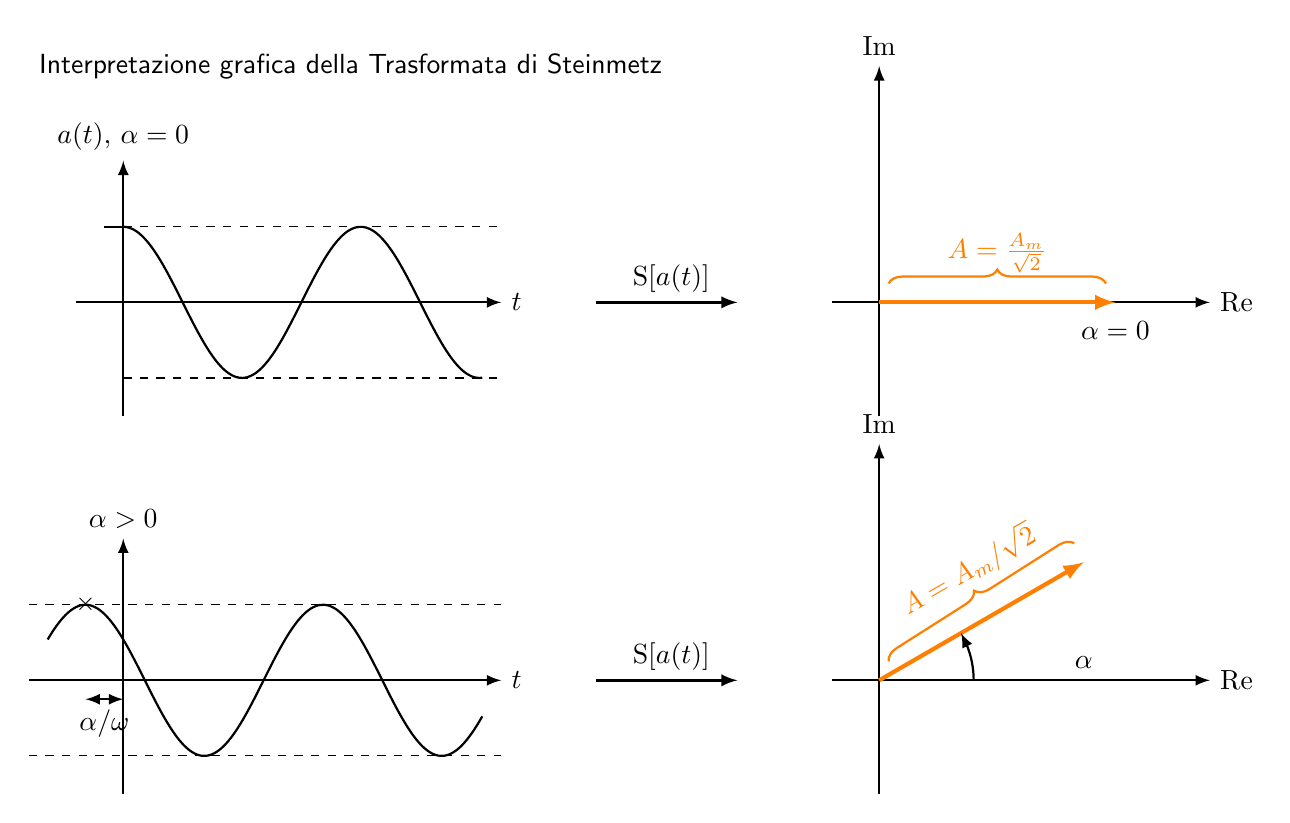
\begin{tikzpicture}[
				thick,
				>=latex,
				scale=1.2,
				phasor/.style={->, line width=1.5pt, color=orange},
				function/.style={color=black, smooth},
				label_text/.style={font=\small\sffamily}
				]
				
				% --- Titolo ---
				\node[anchor=west] at (-1, 2.5) {\sffamily Interpretazione grafica della Trasformata di Steinmetz};
				
				% ==================================================================
				% --- RIGA 1: Caso alfa = 0 ---
				% ==================================================================
				
				% --- Grafico nel tempo (Sinistra) ---
				\begin{scope}
					% Etichette
					\node[above] at (0, 1.5) {$a(t)$, $\alpha=0$};
					
					% Assi
					\draw[->] (-0.5, 0) -- (4, 0) node[right] {$t$};
					\draw[->] (0, -1.2) -- (0, 1.5);
					
					% Linee tratteggiate per l'ampiezza
					\def\Am{0.8}
					\draw[dashed, thin] (0, \Am) -- (4, \Am);
					\draw[dashed, thin] (0, -\Am) -- (4, -\Am);
					
					% Funzione sinusoidale (Coseno con fase 0)
					\draw[function, domain=0:3.8, samples=100] plot (\x, {\Am * cos(deg(2.5*\x))});
					
					% Segno del valore iniziale
					\draw[thick] (0, \Am) -- (-0.2, \Am);
				\end{scope}
				
				% --- Freccia di trasformazione S[...] ---
				\begin{scope}[xshift=5cm, yshift=0cm]
					\node[above] at (0.8, 0) {S[$a(t)$]};
					\draw[->, line width=1pt] (0, 0) -- (1.5, 0);
				\end{scope}
				
				% --- Piano dei Fasori (Destra) ---
				\begin{scope}[xshift=8cm, yshift=0cm]
					% Assi Re/Im
					\draw[->] (-0.5, 0) -- (3.5, 0) node[right] {Re};
					\draw[->] (0, -1.2) -- (0, 2.5) node[above] {Im};
					\coordinate (O) at (0,0);
					
					% Fasore (su asse Reale)
					\draw[phasor] (O) -- (2.5, 0) node[right, below= 3 pt,black] {$\alpha=0$};
					
					% Etichetta Ampiezza A
					% Linea ondulata arancione per indicare la lunghezza
					\draw[orange, decorate, decoration={brace, amplitude=5pt}] (0.1, 0.2) -- (2.4, 0.2);
					\node[above, orange] at (1.25, 0.2) {$A=\frac{A_m}{\sqrt{2}}$};
				\end{scope}
				
				
				% ==================================================================
				% --- RIGA 2: Caso alfa > 0 ---
				% ==================================================================
				
				\begin{scope}[yshift=-4cm] % Sposta tutto giù di 4cm
					
					% --- Grafico nel tempo (Sinistra) ---
					\begin{scope}
						% Etichette
						\node[above] at (0, 1.5) {$\alpha>0$};
						
						% Assi
						\draw[->] (-1, 0) -- (4, 0) node[right] {$t$};
						\draw[->] (0, -1.2) -- (0, 1.5);
						
						% Linee tratteggiate
						\def\Am{0.8}
						\draw[dashed, thin] (-1, \Am) -- (4, \Am);
						\draw[dashed, thin] (-1, -\Am) -- (4, -\Am);
						
						% Funzione sinusoidale sfasata (Coseno traslato a sinistra)
						% Fase alfa/w = 0.4 circa nel disegno
						\def\shift{0.4} 
						\draw[function, domain=-0.8:3.8, samples=100] 
						plot (\x, {\Am * cos(deg(2.5*(\x + \shift)))});
						
						% Indicazione dello sfasamento alfa/w
						\draw[<->] (-\shift, -0.2) -- (0, -0.2);
						\node[below] at (-\shift/2, -0.2) {$\alpha/\omega$};
						
						% Segno della croce sul picco traslato
						\node[font=\small] at (-\shift, \Am) {$\times$};
					\end{scope}
					
					% --- Freccia di trasformazione S[...] ---
					\begin{scope}[xshift=5cm, yshift=0cm]
						\node[above] at (0.8, 0) {S[$a(t)$]};
						\draw[->, line width=1pt] (0, 0) -- (1.5, 0);
					\end{scope}
					
					% --- Piano dei Fasori (Destra) ---
					\begin{scope}[xshift=8cm, yshift=0cm]
						% Assi Re/Im
						\draw[->] (-0.5, 0) -- (3.5, 0) node[right] {Re};
						\draw[->] (0, -1.2) -- (0, 2.5) node[above] {Im};
						\coordinate (O) at (0,0);
						
						% Fasore (Sfasato di alfa)
						\def\alfaDeg{30} % Angolo di circa 30 gradi
						\draw[phasor] (O) -- (\alfaDeg:2.5) node[left = 150 pt, below=30 pt, black] {$\alpha$};
						
						% Etichetta Ampiezza A
						\coordinate (P) at (\alfaDeg:2.5);
						% Linea ondulata parallela al fasore
						\draw[orange, decorate, decoration={brace, amplitude=5pt}] 
						($(O)+(0.1, 0.2)$) -- ($(P)+(-0.1, 0.2)$);
						\node[above, orange, rotate=\alfaDeg] at ($(O)!0.5!(P) + (0, 0.3)$) {$A=A_m/\sqrt{2}$};
						
						% Arco per l'angolo alfa
						\draw[->] (1, 0) arc (0:\alfaDeg:1);
					\end{scope}
				\end{scope}
		\end{tikzpicture}
		\caption{Interpretazione grafica della Traformata di Steinmetz}
		\label{fig:steinmetzgraf}
	\end{figure}
\end{dfn}

\begin{dfn}[Antitrasformata di Steinmetz]
	Operatore lineare che associa ad un fasore la sinusoide di pulsazione $\omega$ nota.
	\[S^-1[\underline A] = \sqrt{2} Re(\underline A e^{j\omega t}) =  \sqrt{2} Re(Ae^{j (\omega t + \alpha)}) = A_M cos(\omega t + \alpha) = a(t)\]
	Il numero complesso $f(t) = \sqrt{2}\underline A e^{j\omega t}$ è chiamato \textsl{fasore rotante}. Si veda la \cref{fig:antisteinmetz} per un'interpretazione grafica dell'antitrasformata. L'esponenziale di modulo unitario con fase variabile nel tempo, con pulsazione $\omega$ consente il passaggio al dominio temporale
	\begin{figure}
		\centering
		\includegraphics[width=0.8\linewidth]{antisteinmetz}
		\caption{Interpretazione grafica dell'antitrasformata di Steinmetz}
		\label{fig:antisteinmetz}
	\end{figure}

\end{dfn}
Proprietà della Trasformata di Steinmetz e operazioni con i fasori:
\begin{itemize}
	\item linearità. Si dimostra facilmente dalla linearità della distributività della moltiplicazione tra numeri complessi e dalla linearità dell'operatore integrale.\\
	Se $c(t) = a(t) + b(t)$, $\underline C = \underline A + \underline B = [Re(A) + Re(B)] + j [Im(A) + Im(B)] = \sqrt{\underline A^2 + \underline B^2} e^{j(\alpha_A + \alpha_B)}$.
	\item Moltiplicazione per uno scalare $K \in \mathbb{R}$. $\underline C = K \underline A = K A e^{j\alpha} \iff \begin{cases}
		C=KA\\
		arg(\underline C) = \begin{cases}
			arg(\underline A), k>0\\
			arg(\underline A) + \pi , k<0
		\end{cases}
		\end{cases}$
	\item Moltiplicazione interna (Moltiplicazione per un numero complesse)$\underline Z \in \mathbb{C}= Z A e^{j\alpha_z + \alpha} \iff \begin{cases}
		C=ZA\\
		arg(\underline C) = arg (\underline Z) + arg(\underline A)
	\end{cases}$. 
	\item Trasformata della derivata. 
	\[S[\frac{d}{dt}a(t)] = S[-\omega A_M cos(\omega t + \alpha + \pi/2)] = \omega A_M/\sqrt{2} e^{j\alpha + \pi/2} = \omega \underline A e^{j\pi/2} = j\omega \underline A\]
	In questo modo, le operazioni di derivata temporale vengono ricondotte a operazioni algebriche.
	\[\frac{d}{dt} x(t) \longleftrightarrow j\omega \underline X\]
	\item Trasformata della funzione integrale.\\
	Analogamente,
	\[\int x(t)dt \longleftrightarrow \frac{1}{j\omega} \underline X\]
\end{itemize}
\subsection{Metodo Simbolico}
Possiamo dunque utilizzare trasformata e antitrasformata di Steinmetz per l'analisi di un circuito in regime sinusoidale evitando equazioni integro-differenziali, risolvendo quelle algebriche associate nel campo simbolico (complesso) associato, secondo il percorso in \cref{fig:schema_analisi}
\begin{figure}[H]
	\centering
	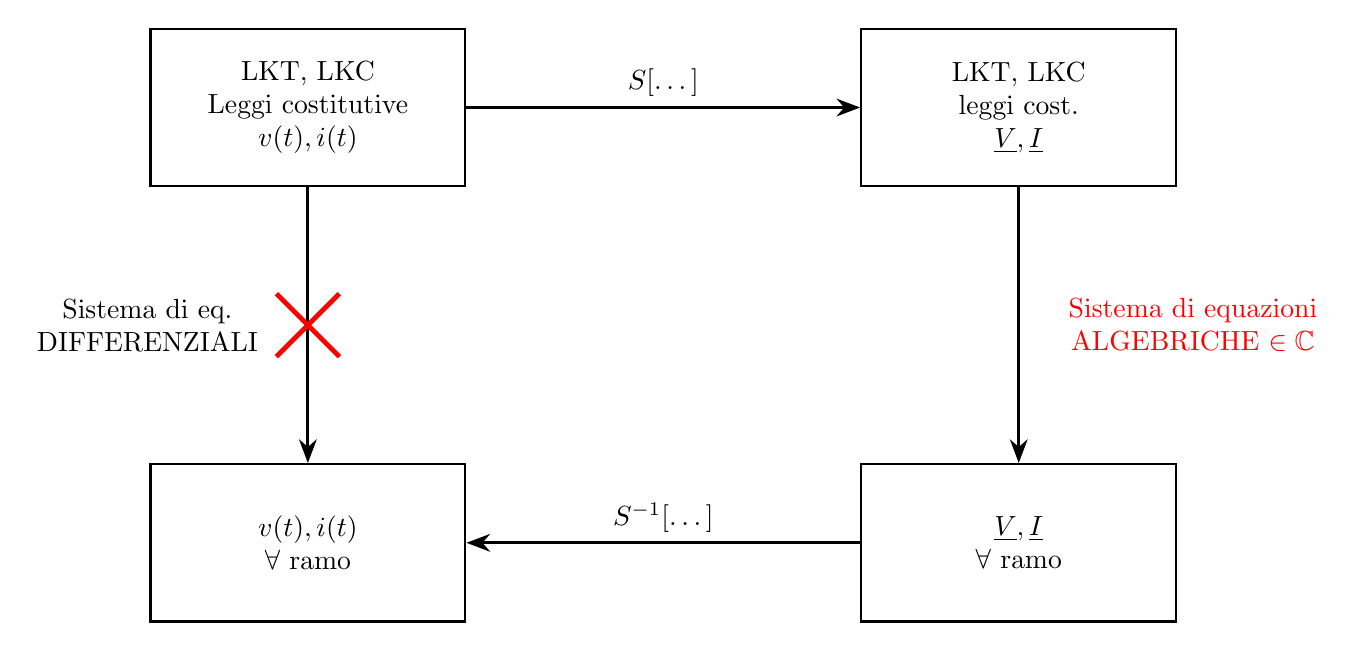
\begin{tikzpicture}[
		node distance = 3.5cm and 5cm,
		box/.style = {
			draw, rectangle, align=center, 
			minimum height=2cm, minimum width=4cm, thick
		},
		arrow/.style = {
			-{Stealth[length=3mm]}, line width=1pt
		}
		]
		
		% Box
		\node[box] (tl) {LKT, LKC \\ Leggi costitutive \\ $v(t), i(t)$};
		\node[box, below=of tl] (bl) {$v(t), i(t)$ \\ $\forall \text{ ramo}$};
		\node[box, right=of tl] (tr) {LKT, LKC \\ leggi cost. \\ $\underline{V}, \underline{I}$};
		\node[box, below=of tr] (br) {$\underline{V}, \underline{I}$ \\ $\forall \text{ ramo}$};
		
		%Frecce ed etichette
		\draw[arrow] (tl) -- node[above, midway] {$S[\dots]$} (tr);
		\draw[arrow] (br) -- node[above, midway] {$S^{-1}[\dots]$} (bl);
		\draw[arrow] (tr) -- node[right, midway, xshift=5mm, align=center, text=red] {Sistema di equazioni \\ ALGEBRICHE $\in \mathbb{C}$} (br);
		\draw[arrow] (tl) -- node[left, midway, xshift=-5mm, align=center] {Sistema di eq. \\ DIFFERENZIALI} (bl);
		
		% X rossa
		\coordinate (mid_left) at ($(tl)!.5!(bl)$);
		\draw[red, line width=1.7pt] (mid_left) +(-4mm, -4mm) -- +(4mm, 4mm);
		\draw[red, line width=1.7pt] (mid_left) +(-4mm, 4mm) -- +(4mm, -4mm);
		
		\end{tikzpicture}
		
		\caption{Schema del percorso di analisi nel dominio del tempo e della frequenza per circuiti in regime sinusoidale applicando il Metodo Simbolico, tramite la Trasformata di Steinmetz}
		\label{fig:schema_analisi}
	\end{figure}
\subsection{Leggi topologiche e costitutive in dominio simbolico}
\begin{legge}[Legge di Kirchhoff delle correnti]
	\[LKC: \sum_{k=1}^n i_k(t) = 0 \quad \xrightarrow{\text{S[...]}} \quad \sum_{k=1}^n \underline I_k(t) = 0 \]
\end{legge}

\begin{legge}[Legge di Kirchhoff delle tensioni]
	\[LKT: \sum_{k=1}^m v_k(t) = 0 \quad \xrightarrow{\text{S[...]}} \quad \sum_{k=1}^n \underline V_k(t) = 0 \]
\end{legge}

\begin{legge}[Legge costitutiva del resistore lineare]
	\[\underline V = R \underline I\]
	Nel campo complesso, dunque, i fasori rappresentativi di corrente e tensione sono in fase (\cref{fig:R_fas}). Nel dominio temporale, saranno rappresentati da due sinusoidi in fase, con ampiezza, in generale, differente (\cref{fig:R_t}). 
	\begin{figure}[H]
		\centering
		
		% --- 1. GRAFICO A SINISTRA (DOMINIO DEL TEMPO - RESISTORE) ---
		\begin{subfigure}[b]{0.6\textwidth}
			\centering
			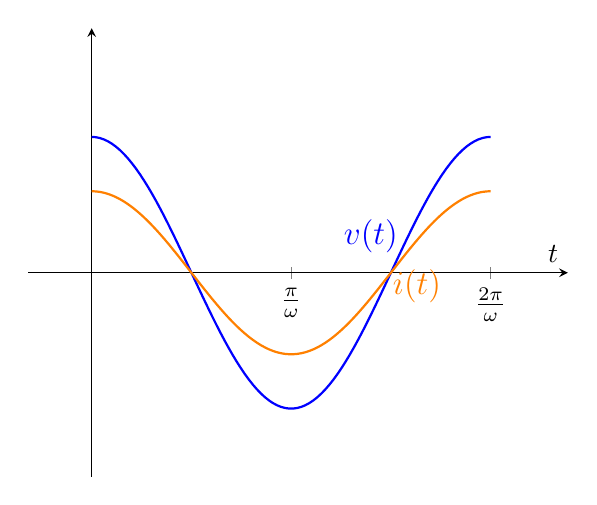
\begin{tikzpicture}
				\begin{axis}[
					axis lines=middle,
					xlabel=$t$,
					xtick = {0, 3.14159, 6.28318},
					xticklabels = {$0$, $\frac{\pi}{\omega}$, $\frac{2\pi}{\omega}$},
					ytick=\empty,
					xmin=-1,
					xmax=7.5,
					ymin=-1.5,
					ymax=1.8,
					clip=false
					]
					
					% --- Funzioni (IN FASE) ---
					% v(t) - sin(x) in BLU
					\addplot[
					blue, thick,
					domain=0:2*pi, 
					samples=100
					] {cos(deg(x))} 
					node[left, pos=0.8, font=\large] {$v(t)$};
					
					% i(t) - 0.6*sin(x) in ARANCIONE
					\addplot[
					orange, thick, 
					domain=0:2*pi, 
					samples=100
					] {0.6*cos(deg(x))} % <- MODIFICA: In fase, ampiezza minore
					node[right, below=7pt, pos=0.82, font=\large] {$i(t)$};
					
					% --- Dettagli (zeri) ---
					% Gli zeri ora si sovrappongono
					\node[blue, mark=x, scale=1.5] at (axis cs:0, 0) {};
					\node[blue, mark=x, scale=1.5] at (axis cs:pi, 0) {};
					\node[blue, mark=x, scale=1.5] at (axis cs:2*pi, 0) {};
					\node[orange, mark=x, scale=1.5] at (axis cs:0, 0) {};
					\node[orange, mark=x, scale=1.5] at (axis cs:pi, 0) {};
					\node[orange, mark=x, scale=1.5] at (axis cs:2*pi, 0) {};
				\end{axis}
			\end{tikzpicture}
			\caption{Grafico nel dominio del tempo (Resistore).}
			\label{fig:R_t}
		\end{subfigure}%
		% --- 2. GRAFICO A DESTRA (FASORI - RESISTORE) ---
		\begin{subfigure}[b]{0.4\textwidth}
			\centering
			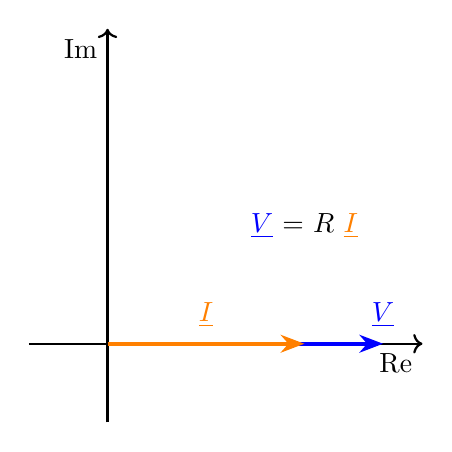
\begin{tikzpicture}[
				thick,
				vettore/.style={-{Stealth[length=3mm]}, line width=1.5pt}
				]
				
				% --- Assi ---
				\draw[->] (-1,0) -- (4,0) node[below left] {Re};
				\draw[->] (0,-1) -- (0,4) node[below left] {Im};
				\coordinate (O) at (0,0);
				
				% --- Vettori (Fasori SOVRAPPOSTI) ---
				% Disegno prima il più lungo (V)
				\draw[vettore, blue] (O) -- (3.5,0) 
				node[above=2pt, blue] {$\underline{V}$};
				% Disegno dopo il più corto (I) per farlo stare sopra
				\draw[vettore, orange] (O) -- (2.5,0) 
				node[midway, above=2pt, orange] {$\underline{I}$};
				
				% --- Etichetta equazione (con colori) ---
				\node at (2.5, 1.5) { % Posizione aggiornata
					\textcolor{blue}{$\underline{V}$} = $R$ \textcolor{orange}{$\underline{I}$}
				};
				
			\end{tikzpicture}
			\caption{Diagramma fasoriale (Resistore).}
			\label{fig:R_fas}
		\end{subfigure}
		
		\caption{Confronto tra dominio del tempo e simbolico per un resistore.}
	\end{figure}
\end{legge}

\begin{legge}[Legge costitutiva del condensatore]
	\[i(t) = C \frac{dv(t)}{dt} \xrightarrow{\text{S[...]}} \begin{aligned}[t] 
		\underline I &= j \omega C \underline V\\
		\underline V &= -\frac{j}{\omega C} \underline I
	\end{aligned}
	\]
	Nel campo complesso, il fasore rappresentativo della corrente è sfasato di $\pi/2$ (in positivo) rispetto alla tensione (\cref{fig:cond_fas}). Nel dominio temporale, dunque, la corrente risulta "in anticipo" di una fase $\pi/2$ rispetto alla tensione (\cref{fig:cond_t}). Si dice anche che il fasore della corrente è \textsl{in quadratura in anticipo} rispetto alla tensione.
	Si ottiene la stessa conclusione considerando che $\frac{d}{dt} cos(t) = -sin(t)$.
	
	\begin{figure}[H]
		\centering
		
		% --- 1. GRAFICO A SINISTRA (DOMINIO DEL TEMPO) ---
		\begin{subfigure}[b]{0.6\textwidth}
			\centering
			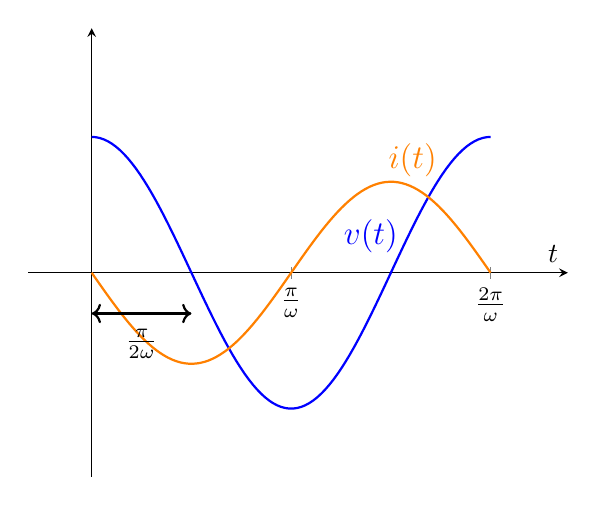
\begin{tikzpicture}
				\begin{axis}[
					axis lines=middle,
					xlabel=$t$,
					% --- MODIFICA: Ticks sull'asse x ---
					xtick = {0, 3.14159, 6.28318},
					xticklabels = {$0$, $\frac{\pi}{\omega}$, $\frac{2\pi}{\omega}$},
					% ---
					ytick=\empty,
					xmin=-1,
					xmax=7.5,
					ymin=-1.5,
					ymax=1.8,
					clip=false
					]
					
					% --- Funzioni ---
					% v(t) - sin(x) in BLU
					\addplot[
					blue, thick, % <- MODIFICA: Colore cambiato
					domain=0:2*pi, 
					samples=100
					] {cos(deg(x))} 
					node[left, pos=0.8, font=\large] {$v(t)$};
					
					% i(t) - cos(x) in arancione
					\addplot[
					orange, thick, 
					domain=0:2*pi, 
					samples=100
					] {-0.67*sin(deg(x))} 
					node[above, pos=0.8, font=\large] {$i(t)$};
					
					% --- Dettagli (zeri) ---
					% Segni 'x' per gli zeri
					\node[blue, mark=x, scale=1.5] at (axis cs:0, 0) {};
					\node[blue, mark=x, scale=1.5] at (axis cs:pi, 0) {};
					\node[blue, mark=x, scale=1.5] at (axis cs:2*pi, 0) {};
					\node[orange, mark=x, scale=1.5] at (axis cs:pi/2, 0) {};
					\node[orange, mark=x, scale=1.5] at (axis cs:1.5*pi, 0) {};
					
					% --- Frecce sui picchi rimosse ---
					
					% Freccia e etichetta fase
					\draw[<->, thick] 
					(axis cs:0, -0.3) -- (axis cs:{pi/2}, -0.3) 
					node[midway, below=2pt] {$\frac{\pi}{2\omega}$};
				\end{axis}
			\end{tikzpicture}
			\caption{Grafico nel dominio del tempo.}
			\label{fig:cond_t}
		\end{subfigure}%
		% --- 2. GRAFICO A DESTRA (FASORI) ---
		\begin{subfigure}[b]{0.4\textwidth}
			\centering
			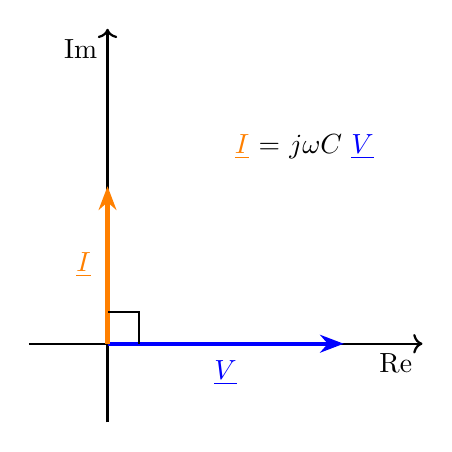
\begin{tikzpicture}[
				thick,
				vettore/.style={-{Stealth[length=3mm]}, line width=1.5pt}
				]
				
				% --- Assi ---
				\draw[->] (-1,0) -- (4,0) node[below left] {Re};
				\draw[->] (0,-1) -- (0,4) node[below left] {Im};
				\coordinate (O) at (0,0);
				
				% --- Vettori (Fasori) ---
				% Fasore V in BLU
				\draw[vettore, blue] (O) -- (3,0) 
				node[midway, below=2pt, blue] {$\underline{V}$};
				% Fasore I in ARANCIONE
				\draw[vettore, orange] (O) -- (0,2) 
				node[midway, left=2pt, orange] {$\underline{I}$};
				
				% --- Etichetta equazione (con colori) ---
				\node at (2.5, 2.5) {
					\textcolor{orange}{$\underline{I}$} = $j\omega C$ \textcolor{blue}{$\underline{V}$}
				};
				
				% --- Angolo retto ---
				\coordinate (A) at (0.4, 0);
				\coordinate (B) at (0, 0.4);
				\draw (A) -- (0.4, 0.4) -- (B);
				
			\end{tikzpicture}
			\caption{Diagramma fasoriale.}
			\label{fig:cond_fas}
		\end{subfigure}
		\caption{Confronto tra dominio del tempo e dominio simbolico per un condensatore.}
	\end{figure}
\end{legge}

\begin{legge}[Legge costitutiva dell'induttore]
	\[v(t) = L \frac{di(t)}{dt} \xrightarrow{\text{S[...]}} \begin{aligned}[t] 
		\underline V &= j \omega L \underline I\\
		\underline I &= - j \frac{\underline V}{\omega L}
	\end{aligned}
	\]
	Nel campo complesso, il fasore rappresentativo della corrente è sfasato di $\pi/2$ (in negativo) rispetto alla tensione (\cref{fig:ind_fas}). Nel dominio temporale, dunque, la corrente risulta "in anticipo" di una fase $\pi/2$ rispetto alla tensione (\cref{fig:ind_t}). Si dice anche che il fasore della corrente è \textsl{in quadratura in ritardo} rispetto alla tensione.
	Si ottiene la stessa conclusione considerando che $\frac{d}{dt} cos(t) = -sin(t)$.
	
	\begin{figure}[H]
		\centering
		
		% --- 1. GRAFICO A SINISTRA (DOMINIO DEL TEMPO) ---
		\begin{subfigure}[b]{0.6\textwidth}
			\centering
			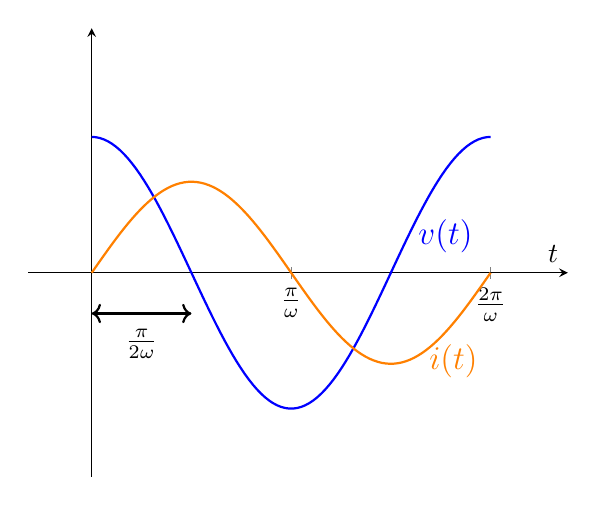
\begin{tikzpicture}
				\begin{axis}[
					axis lines=middle,
					xlabel=$t$,
					% --- MODIFICA: Ticks sull'asse x ---
					xtick = {0, 3.14159, 6.28318},
					xticklabels = {$0$, $\frac{\pi}{\omega}$, $\frac{2\pi}{\omega}$},
					% ---
					ytick=\empty,
					xmin=-1,
					xmax=7.5,
					ymin=-1.5,
					ymax=1.8,
					clip=false
					]
					
					% --- Funzioni ---
					% v(t) - sin(x) in BLU
					\addplot[
					blue, thick, % <- MODIFICA: Colore cambiato
					domain=0:2*pi, 
					samples=100
					] {cos(deg(x))} 
					node[right, pos=0.8, font=\large] {$v(t)$};
					
					% i(t) - cos(x) in arancione
					\addplot[
					orange, thick, 
					domain=0:2*pi, 
					samples=100
					] {0.67*sin(deg(x))} 
					node[right, below=4pt, pos=0.9, font=\large] {$i(t)$};
					
					% --- Dettagli (zeri) ---
					% Segni 'x' per gli zeri
					\node[blue, mark=x, scale=1.5] at (axis cs:0, 0) {};
					\node[blue, mark=x, scale=1.5] at (axis cs:pi, 0) {};
					\node[blue, mark=x, scale=1.5] at (axis cs:2*pi, 0) {};
					\node[orange, mark=x, scale=1.5] at (axis cs:pi/2, 0) {};
					\node[orange, mark=x, scale=1.5] at (axis cs:1.5*pi, 0) {};
					
					% --- Frecce sui picchi rimosse ---
					
					% Freccia e etichetta fase
					\draw[<->, thick] 
					(axis cs:0, -0.3) -- (axis cs:{pi/2}, -0.3) 
					node[midway, below=2pt] {$\frac{\pi}{2\omega}$};
				\end{axis}
			\end{tikzpicture}
			\caption{Grafico nel dominio del tempo.}
			\label{fig:ind_t}
		\end{subfigure}%
		% --- 2. GRAFICO A DESTRA (FASORI) ---
		\begin{subfigure}[b]{0.4\textwidth}
			\centering
			\begin{tikzpicture}[
				thick,
				vettore/.style={-{Stealth[length=3mm]}, line width=1.5pt}
				]
				
				% --- Assi ---
				\draw[->] (-1,0) -- (4,0) node[below left] {Re};
				\draw[->] (0,-1) -- (0,4) node[below left] {Im};
				\coordinate (O) at (0,0);
				
				% --- Vettori (Fasori) ---
				% Fasore V in BLU
				\draw[vettore, blue] (O) -- (3,0) 
				node[midway, below=2pt, blue] {$\underline{V}$};
				% Fasore I in ARANCIONE
				\draw[vettore, orange] (O) -- (0,-2) 
				node[midway, left=2pt, orange] {$\underline{I}$};
				
				% --- Etichetta equazione (con colori) ---
				\node at (2.5, 2.5) {
					\textcolor{orange}{$\underline{I}$} = $j\omega L$ \textcolor{orange}{$\underline{I}$}
				};
				
				% --- Angolo retto ---
				\coordinate (A) at (0.4, 0);
				\coordinate (B) at (0, 0.4);
				\draw (A) -- (0.4, 0.4) -- (B);
				
			\end{tikzpicture}
			\caption{Diagramma fasoriale.}
			\label{fig:ind_fas}
		\end{subfigure}
		\caption{Confronto tra dominio del tempo e dominio simbolico per un induttore.}
	\end{figure}
\end{legge}

\subsection{Legge di Ohm simbolica}
Osserviamo, dunque, che per i componenti descritti sopra, i fasori tensione e corrente sono sempre proporzionali, con costanti diverse (\cref{fig:impedenza}). Definiamo dunque l'\textsl{impedenza} come tale costante di proporzionalità. Questa grandezza ci sarà utile per formulare l'equivalente della Legge di Ohm in dominio simbolico. 
\begin{figure}[H]
	\centering
	\includegraphics[width=0.7\linewidth]{impedenza}
	\caption{}
	\label{fig:impedenza}
\end{figure}

\begin{dfn}[Impedenza]
	Definiamo \textsl{Impedenza} $\underline Z \in \mathbb{C}$
	\[\underline Z = \frac{\underline V}{\underline I}\]
	Essa rappresenta quanto il bipolo a cui è riferita si oppone al passaggio di una corrente alternata in regime sinusoidale.\\
	Chiamiamo \textsl{sfasamento} la quantità $\varphi = arg(\underline Z) = \alpha_V - \alpha_I$ e \textsl{reattanza} la parte immaginaria dell'impedenza, mentre notiamo che la parte reale dell'impedenza coincide con la resistenza del componente. La reattanza può assumere qualunque valore reale. La resistenza di un componente non è mai negativa, ma nell'analisi dei circuiti equivalenti che condurremo in seguito è possibile che emergano resistenze negative.
	\[\underline Z = \frac{V}{I}e^{j(\alpha_V - \alpha_I)} = Z cos(\varphi) + jZ sin(\varphi) = R + j X\]
	Seguendo il procedimento contrario,
	\[\begin{aligned}
		&Z = |\underline Z| = \sqrt{R^2 + X^2}\\
		&\varphi = \arg(\underline Z) = \begin{cases}
			atan(X/R), R>0\\
			atan(X/R) \pm \pi, R<0
		\end{cases}
	\end{aligned}\]
	
	Studiamo l'impedenza dei bipoli considerati.
	\begin{itemize}
		\item Per un resistore, \[
		\begin{aligned}
			&Z_R = R\\
			&\varphi_R = arg (\underline Z_R) = 0
		\end{aligned}\]
		Un bipolo di questo tipo, con reattanza nulla, è detto \textsl{ohmico};
		\item Per un condensatore, la resistenza è nulla. Si osservi che la reattanza è negativa.
		\[\underline Z_C = -\frac{j}{\omega C} =  X_C \iff 
		\begin{aligned}
			&Z_C = \frac{1}{\omega C}\\
			&\varphi_C = arg(\underline Z_C) = -\frac{\pi}{2}
		\end{aligned}\]
		\item Per un induttore, la resistenza è nulla. Si osservi che la (reattanza) è positiva
		\[\underline Z_L = j\omega L =  X_L \iff 
		\begin{aligned}
			&Z_L = \omega L\\
			&\varphi_L = arg(\underline Z_L) = \frac{\pi}{2}
		\end{aligned}\]
	\end{itemize}
\end{dfn}
\begin{dfn}[Ammettenza]
	Analogamente a come abbiamo introdotto la conduttanza come reciproco della resistenza, definiamo l'\textsl{Ammettenza}
	\[\underline Y = \frac{1}{\underline Z} = \frac{I}{V} e^{j (-\varphi)} = \frac{R}{R^2 + X^2} + j (-\frac{X}{R^2 + X^2})= G + jB\]
	dove $G$ è la conduttanza, e coincide con $1/R$ nel caso di un bipolo ohmico; e $B$ è detto \textsl{suscettanza} e in caso di bipolo induttivo o capacitivo $B=-1/X$.
\end{dfn}

\begin{legge}[Legge di Ohm simbolica]
	Con riferimento al bipolo generico in \cref{fig:ohmsimb} con la convenzione dell'utilizzatore, valgono le seguenti relazioni, che esprimono la Legge di Ohm in dominio simbolico:
	\[\underline V = \underline Z \underline I \quad \longleftrightarrow \quad v=Ri\]
	\[\underline I = \underline Y \underline V \quad \longleftrightarrow \quad i = Gv\]	
	\begin{figure}[H]
		\centering
		\includegraphics[width=0.5\linewidth]{ohm_simb}
		\caption{}
		\label{fig:ohmsimb}
	\end{figure}
\end{legge}

\begin{ex}
	Con riferimento al circuito in \cref{fig:circsimb}
	\begin{itemize}
		\item Trovare i fasori delle correnti in tutti i rami del circuito
		\item Determinare l'andamento temporale di $i_{g1}(t)$
	\end{itemize}
	\begin{figure}[H]
		\centering
		\includegraphics[width=0.7\linewidth]{circsimb}
		\caption{$R_1 = 1\ \Omega$, $R_2 = 2\ Omega$, $L=1\ mH$, $C= 1\ mF$, $V_{g1}= 12\sqrt{2} cos(\omega t + \pi/2)$ , $\omega = 2\pi f$, $f=10^3\ rad/s$ }
		\label{fig:circsimb}
	\end{figure}
	
	Soluzione. Come indicato nello schema in \cref{fig:schema_analisi}: 
	\begin{itemize}
		\item [1.]Circuito in dominio simbolico
		\item [2.]Trasformazione di Steinmetz delle leggi costitutive
		\item [3.]Soluzione di $\underline V, \underline I$
		\item [4.] Antitrasformazione di Steinmetz per ottenere $v(t), i(t)$.
	\end{itemize}
	
	Dunque, per la risoluzione dell'esercizio, si può scrivere il sistema:
	\[\begin{cases}
		\underline V_{g1} = S[V_{g1}] = 12 e^{j\pi/2} = j12\\
		\underline Z_{R1} = 1\\
		\underline Z_{R2} = 2\\
		\underline Z_L = j\omega L = j\\
		\underline Z_C = \frac{j}{\omega C} = -j\\		
	\end{cases}\]
	
	Osserviamo che le semplificazioni in serie e parallelo utilizzate per resistori, funzionano in maniera analoga per le impedenze:
	\[\begin{aligned}
		&\underline Z_{serie} = \sum_k \underline Z_k\\
		&\underline Z_{parallelo} = \frac{1}{\sum_k \frac{1}{\underline Z_k}}
	\end{aligned}\]
	Semplificando il nostro circuito, otteniamo:
	\[\begin{aligned}
		\begin{cases}
			\underline Z_{eq1} = Z_{R1} + \underline Z_L = 1+j\\
			\underline Z_{eq2} = \frac{\underline Z_C Z_{R2}}{\underline Z_C+ Z_{R2}} = 0,4 - j0,8\\
		\end{cases}\\
		\underline Z_{eq3} = \underline Z_{eq1} + \underline Z_{eq2} = 1,4 + j0,2\\
	\end{aligned}
	\]
	Risulta dunque:
	\[\underline I_{g1} = \frac{\underline V_{g1}}{\underline Z_{eq3}} = 1,2 + j 8,4\]
	Facendo riferimento al circuito originario,
	\[\begin{cases}
		\underline I_{R1} = \underline I_L = \underline I_{g1}\\
		\underline I_C = \underline I_{g1}\frac{Z_{R2}}{\underline Z_{R2} + \underline Z_C} = -2,4 + j 7,2\\
		\underline I_{R2} = \underline I_{g1} - \underline I_C = 3,6 + j 1,2
	\end{cases}\]
	E infine, considerando che
	\[\begin{cases}
		I_{g1} = \sqrt{Re(\underline I_{g1})^2 + Im(\underline I_{g1}^2)}= \sqrt{1,2^2 + 8,4^2} = 8,49\ A\\
		arg(\underline I_{g1}) = atan(8,4/1,2) = 1,43\ rad\\
	\end{cases}
	\]
	si ottiene:
	\[i_{g1}(t) = S^{-1}[\underline I_{g1}] = \sqrt{2} I_{g1} cos(\omega t + arg (\underline I_{g1})) =\sqrt{2} I_{g1} cos(\omega t + arg (\underline I_{g1})) =8,49\sqrt{2}  cos(2000\pi t + 1,43)\ A\]
\end{ex}
\subsection{Potenza in regime sinusoidale}
In generale, sappiamo che $p_A(t) = v(t) i(t)\quad (W)$.
In regime sinusoidale, tuttavia è possibile trovarne un'espressione più funzionale.
Consideriamo $\alpha_V = 0$ e $\alpha_I = -\varphi$, per semplificare i calcoli, senza perdita di generalità. Consideriamo una corrente in ritardo perché, generalmente, nelle applicazioni pratiche, la corrente è effettivamente in ritardo, perché i sistemi sono dominati da componente induttiva.\\
\[\begin{aligned}
	&v(t) = V_M cos(\omega t)\\
	&i(t) = I_M cos(\omega t - \varphi) = I_Mcos(\omega t)cos(\varphi) + I_M sin(\omega t)sin(varphi)=i_a(t) + i_r(t)
\end{aligned}\]
Chiamiamo il primo termine della corrente,  $i_a(t)$, in fase con la tensione, \textsl{corrente attiva}, mentre il secondo termine, $i_r(t)$, in quadratura con la tensione \textsl{corrente reattiva}.
\[p(t) = v(t)\cdot (i_a(t) + i_r(t) = v(t)i_a(t) + v(t)i_r(t)\]
Studiamo ora i due termini dell'espressione della potenza.

\begin{dfn}[Potenza istantanea attiva]
	Chiamiamo \textsl{potenza istantanea attiva} il termine:
	\[p_a(t) = v(t)i_a(t) = V_Mcos(\omega t)I_M cos(\omega t)cos(\varphi) = V_MI_Mcos^2(\omega t)cos(\varphi)=\frac{V_MI_M}{2}[1 + cos(2\omega t)]cos(\varphi)\]
	Da considerazioni analitiche, o dalla rappresentazione in \cref{fig:pot_att}, si osserva che:
	\begin{itemize}
		\item ha frequenza doppia rispetto a $v(t)$ e $i(t)$
		\item ha valore medio $\neq 0$
		\item è \textsl{unidirezionale} ($p_a(t) \geq 0 \quad \forall t$)
		\item $w(t) = \int p(t)dt \geq 0$ (ombreggiato in \cref{fig:pot_att}).
		\item essa è associata ai bipoli ohmici, o alla componente ohmica di bipoli non puri.
	\end{itemize}
	Per questo si conclude che la potenza istantanea attiva produce un lavoro "utile".
	
	\begin{figure}[H]
		\centering
		\begin{subfigure}[b]{0.8\textwidth}
			\centering
			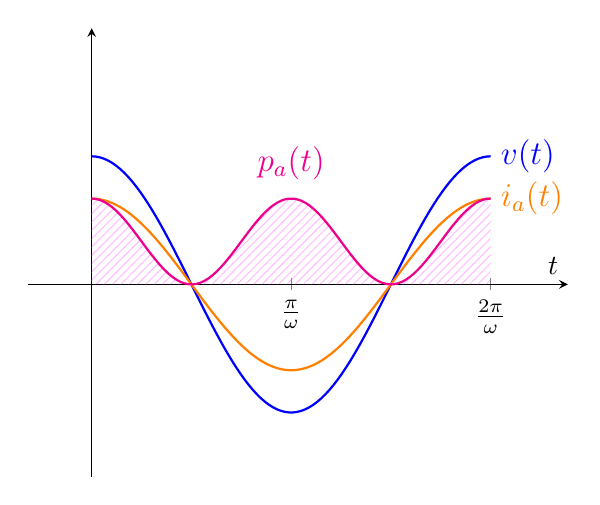
\begin{tikzpicture}
				\begin{axis}[
					axis lines=middle,
					xlabel=$t$,
					% --- MODIFICA: Ticks sull'asse x ---
					xtick = {0, 3.14159, 6.28318},
					xticklabels = {$0$, $\frac{\pi}{\omega}$, $\frac{2\pi}{\omega}$},
					% ---
					ytick=\empty,
					xmin=-1,
					xmax=7.5,
					ymin=-1.5,
					ymax=2.0,
					clip=false
					]
					
					% --- Funzioni ---
					% v(t) - sin(x) in BLU
					\addplot[
					blue, thick, % <- MODIFICA: Colore cambiato
					domain=0:2*pi, 
					samples=100
					] {cos(deg(x))} 
					node[right, font=\large] {$v(t)$};
					
					% i(t) - cos(x) in arancione
					\addplot[
					orange, thick, 
					domain=0:2*pi, 
					samples=100
					] {0.67*cos(deg(x))} 
					node[right, font=\large] {$i_a(t)$};
					
					\addplot[
					magenta, thick, 
					domain=0:2*pi, 
					samples=100,
					name path=plotp,
					] {0.67*(1 + cos(deg(2*x)))*0.5} 
					node[above=3pt, pos= 0.5, font=\large] {$p_a(t)$};
					\path[name path=xaxis] (axis cs:0,0) -- (axis cs:2*pi,0);
					\addplot[
					pattern=north east lines,   % Stile tratteggio
					pattern color=magenta!60,      % Colore del tratteggio
					opacity=0.4                 % Leggera trasparenza
					] 
					fill between[
					of = plotp and xaxis,       % Riempie tra 'plot_v' e l'asse x
					soft clip={domain=0:2*pi}   % Solo nel dominio della funzione
					];
					
					% --- Dettagli (zeri) ---
					% Segni 'x' per gli zeri
					\node[blue, mark=x, scale=1.5] at (axis cs:0, 0) {};
					\node[blue, mark=x, scale=1.5] at (axis cs:pi, 0) {};
					\node[blue, mark=x, scale=1.5] at (axis cs:2*pi, 0) {};
					\node[orange, mark=x, scale=1.5] at (axis cs:pi/2, 0) {};
					\node[orange, mark=x, scale=1.5] at (axis cs:1.5*pi, 0) {};
					
				\end{axis}
			\end{tikzpicture}
		\end{subfigure}
		\caption{Possibile andamento della potenza istantanea attiva, per valori arbitrari di $V_M$, $I_M$ e $cos(\varphi)$. Si osservi che nel caso estremale in cui }
		\label{fig:pot_att}
	\end{figure}
\end{dfn}

\begin{dfn}[Potenza istantanea reattiva]
	Chiamiamo \textsl{potenza istantanea reattiva} il termine:
	\[p_r(t) = v(t)i_r(t) = V_Mcos(\omega t)I_M sin(\omega t)sin(\varphi) =\frac{V_MI_M}{2}sin(2\omega t)sin(\varphi)\]
	Da considerazioni analitiche, o dalla rappresentazione in \cref{fig:pot_reatt}, si osserva che:
	\begin{itemize}
		\item ha frequenza doppia rispetto a $v(t)$ e $i(t)$
		\item ha valore medio $= 0$
		\item è \textsl{bidirezionale} ($p_a(t) \gtrless 0$)
		\item $w(t) = \int_{-T/2}^{T/2} p(t)dt = 0$ (ombreggiato in \cref{fig:pot_reatt}).
		\item essa è associata ai bipoli reattivi, o alla componente reattiva di bipoli non puri.
	\end{itemize}
	Per questo si conclude che la potenza istantanea reattiva non produce lavoro utile (perché non produce lavoro netto).
	
	\begin{figure}[H]
		\centering
		\begin{subfigure}[b]{0.8\textwidth}
			\centering
			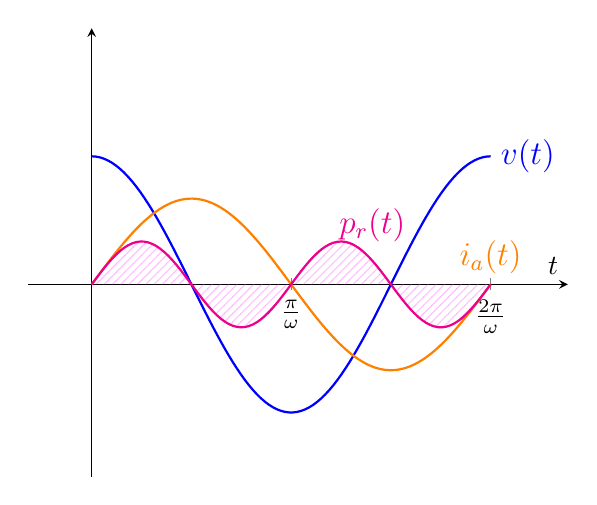
\begin{tikzpicture}
				\begin{axis}[
					axis lines=middle,
					xlabel=$t$,
					% --- MODIFICA: Ticks sull'asse x ---
					xtick = {0, 3.14159, 6.28318},
					xticklabels = {$0$, $\frac{\pi}{\omega}$, $\frac{2\pi}{\omega}$},
					% ---
					ytick=\empty,
					xmin=-1,
					xmax=7.5,
					ymin=-1.5,
					ymax=2.0,
					clip=false
					]
					
					% --- Funzioni ---
					% v(t) - sin(x) in BLU
					\addplot[
					blue, thick, % <- MODIFICA: Colore cambiato
					domain=0:2*pi, 
					samples=100
					] {cos(deg(x))} 
					node[right, font=\large] {$v(t)$};
					
					% i(t) - cos(x) in arancione
					\addplot[
					orange, thick, 
					domain=0:2*pi, 
					samples=100
					] {0.67*sin(deg(x))} 
					node[above, font=\large] {$i_a(t)$};
					
					\addplot[
					magenta, thick, 
					domain=0:2*pi, 
					samples=100,
					name path=plotp,
					] {0.67*sin(deg(2*x))*0.5} 
					node[above=3pt, pos= 0.7, font=\large] {$p_r(t)$};
					
					\path[name path=xaxis] (axis cs:0,0) -- (axis cs:2*pi,0);
					\addplot[
					pattern=north east lines,   % Stile tratteggio
					pattern color=magenta!60,      % Colore del tratteggio
					opacity=0.4                 % Leggera trasparenza
					] 
					fill between[
					of = plotp and xaxis,       % Riempie tra 'plot_v' e l'asse x
					soft clip={domain=0:2*pi}   % Solo nel dominio della funzione
					];
					% --- Dettagli (zeri) ---
					% Segni 'x' per gli zeri
					\node[blue, mark=x, scale=1.5] at (axis cs:0, 0) {};
					\node[blue, mark=x, scale=1.5] at (axis cs:pi, 0) {};
					\node[blue, mark=x, scale=1.5] at (axis cs:2*pi, 0) {};
					\node[orange, mark=x, scale=1.5] at (axis cs:pi/2, 0) {};
					\node[orange, mark=x, scale=1.5] at (axis cs:1.5*pi, 0) {};
					
				\end{axis}
			\end{tikzpicture}
		\end{subfigure}
		\caption{Possibile andamento della potenza istantanea reattiva, per valori arbitrari di $V_M$, $I_M$ e $cos(\varphi)$}
		\label{fig:pot_reatt}
	\end{figure}
\end{dfn}
Ricapitolando:
\begin{itemize}
	\item Per componenti ohmici ($R$), la potenza è attiva, e il lavoro è dissipato in forma di energia termica.
	\item Per componenti reattivi ($L$, $C$), la potenza è reattiva e il lavoro compiuto è trasferimento di energia tra i componenti, ed è immagazzinata come energia elettrostatica ($C$) o magnetica ($L$); in alcune fasi assorbono energia, in una altra la restituiscono al generatore: il flusso è bidirezionale, e la bidirezionalità è necessaria al funzionamento del componente all'inversione della polarità.
\end{itemize}
\begin{dfn}[Potenza attiva]
	Chiamiamo \textsl{Potenza attiva} il valor medio della potenza istantanea su un periodo.
	\begin{multline*}
		P = \frac{1}{T} \int_{\frac{T}{2}}^{\frac{T}{2}} [\frac{V_MI_M}{2}[1 + cos(2\omega t)] cos(\varphi) +  \frac{V_MI_M}{2}sin(2\omega t) sin(\varphi)] =\\
		= \frac{1}{T} \int_{\frac{T}{2}}^{\frac{T}{2}} [\frac{V_MI_M}{2}cos(\varphi) = \frac{V_MI_M}{2}cos(\varphi) = VIcos(\varphi)
	\end{multline*}
	
	Si osserva dunque l'utilità dell'introduzione dei valori efficaci nella trattazione del regime sinusoidale: consentono di esprimere la potenza attiva in una forma più compatta.\\
	Ci si riferisce comunemente a valori efficaci anche nel quotidiano, quando si dice che la tensione in un impianto domestico è $230\ V$ (una volta $220\ V$).
	Il fattore $\cos(\varphi)$ è detto \textsl{fattore di potenza}. 
	\begin{itemize}
		\item $\varphi = 0$: se $v(t)$ e $i(t)$ sono in fase, $cos(\varphi)=1 \Rightarrow P=VI$;
		\item $varphi = \frac{pi}{2}$: se $i(t)$ è in quadratura in ritardo su $v(t)$, $cos(\varphi)=0 \Rightarrow P=0 \forall V, I$.
	\end{itemize}
\end{dfn}

\begin{dfn}[Potenza reattiva]
	Chiamiamo \textsl{Potenza reattiva} l'ampiezza della potenza istantanea reattiva.
	\[Q = \frac{V_MI_M}{2}sin(\varphi) = VIsin(\varphi) \quad (VA_r)\]
	$Q$ è misurata in $VA_r$, \textsl{Volt-Ampère reattivi}. $Q$ misura l'entità dello scambio di potenza istantanea reattiva tra componenti reattivi e generatori.
	 \begin{itemize}
	 	\item $\varphi = 0$: se $v(t)$ e $i(t)$ sono in fase, $Q=0$;
	 	\item $varphi = \frac{pi}{2}$: se $i(t)$ è in quadratura in ritardo rispetto a $v(t)$ sono in quadratura, $Q=VI$.
	 \end{itemize}
\end{dfn}

\begin{dfn}[Potenza complessa]
	\[\underline N = \underline V \underline I^* = Ve^{j\alpha_V}Ie^{j\alpha_I} = VIe^{j\varphi} = VIcos(\varphi) + jVIsin(\varphi) = P + jQ\]
	Risulta dunque:
	\[\begin{cases}
		P = Re(\underline N)\\
		Q = Im(\underline N)
	\end{cases}\]
\end{dfn}
Nel caso di generatori, l'unica relazione impiegabile in dominio complesso è (con convenzione del generatore),:
\[\underline N_E = \underline V \underline I^*\]
Nel caso di bipoli passivi (con convenzione dell'utilizzatore),
\[\underline N_A = \underline V \underline I^* = \underline Z I^2 = RI^2 + jXI^2\]
\begin{itemize}
	\item Resistore: $Z_R = R \Rightarrow \underline N_{A,R} = Z_R I^2 = RI^2$;
	\item Induttore: $Z_L = j\omega L \Rightarrow \underline N_{A,L} = \underline Z_L I^2 = j \omega L I^2 \quad (Q=\omega LI^2 > 0)$;
	\item Condensatore: $Z_C = -\frac{j}{\omega C} \Rightarrow \underline N_{A,C} = \underline Z_C I^2 = -\frac{j}{\omega C} I^2 \quad (Q=-\frac{1}{\omega C} I^2 < 0)$;
\end{itemize}

È possibile disegnare il numero complesso $\underline N$ su un piano denominato \textsl{triangolo delle potenze} (\cref{fig:tr_pot}). L'angolo di $\underline N$ con l'asse reale è $\varphi$, la proiezione di $\underline N$ sull'asse reale è $P$, quello sull'asse immaginario $Q$.
$N = |\underline N| = \sqrt{P^2 + Q^2} \quad (VA)$ è detto \textsl{potenza apparente}, e rappresenta l'entità delle sollecitazioni subite dal componente. Le caratteristiche di carico di un trasformatore sono spesso espresse proprio in $VA$.

\begin{figure}
	\centering
	\begin{subfigure}[b]{0.4\textwidth}
		\centering
		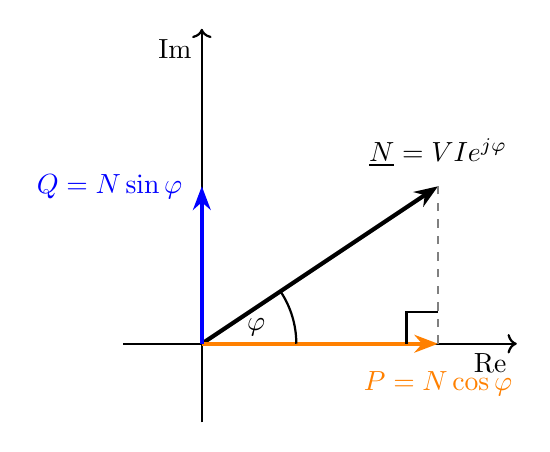
\begin{tikzpicture}[
			thick,
			vettore/.style={-{Stealth[length=3mm]}, line width=1.5pt},
			% Stile per l'arco dell'angolo
			angolo_phi/.style={
				draw, -, % Aggiunge frecce all'arco
				angle radius=1.2cm % Controlla la dimensione dell'arco
			}
			]
			
			% --- Assi ---
			\draw[->] (-1,0) -- (4,0) node[below left] {Re};
			\draw[->] (0,-1) -- (0,4) node[below left] {Im};
			\coordinate (O) at (0,0);
			
			% --- Vettori (Fasori) ---
			% Aggiungo 'coordinate (N_end)' per salvare il punto finale
			\draw[vettore, black] (O) -- (3,2) coordinate (N_end) 
			node[above= 3pt, black] {$\underline{N} = VI e^{j\varphi}$};
			
			% Aggiungo 'coordinate (P_end)'
			\draw[vettore, orange] (O) -- (3,0) coordinate (P_end) 
			node[below=6pt, orange] {$P=N\cos\varphi$}; % Nota: \cos (con \)
			
			\draw[vettore, blue] (O) -- (0,2) 
			node[left= 3pt, blue] {$Q=N\sin\varphi$}; % Nota: \sin (con \)
			
			% --- (Opzionale) Linea tratteggiata per chiudere il triangolo ---
			\draw[dashed, gray] (P_end) -- (N_end);
			
			% --- SOLUZIONE: Disegno dell'angolo \varphi ---
			% Questo 'pic' disegna un arco tra P_end, O (vertice), e N_end
			% e lo etichetta "$\varphi$"
			\pic[
			angolo_phi, % Applica lo stile
			"$\varphi$" % Etichetta
			] 
			{angle = P_end--O--N_end};
			
			% --- (Opzionale) Angolo retto ---
			\pic[
			draw, 
			angle radius=0.4cm, 
			pic text={} % Nessun testo
			] 
			{right angle = N_end--P_end--O};
			
		\end{tikzpicture}
	\end{subfigure}
	\caption{Triangolo delle potenze.}
	\label{fig:tr_pot}
\end{figure}

\begin{ex}
	Facendo riferimento alla \cref{fig:expot}
	\begin{itemize}
		\item calcolare i fasori delle correnti in tutti i rami del circuito 
		\item verificare la conservazione della potenza complessa
		\[\sum \underline N_E = \sum \underline N_A\]
		\[\begin{cases}
			\sum \underline P_E = \sum \underline P_A\\
			\sum \underline Q_E = \sum \underline Q_A
		\end{cases}
		\]
	\end{itemize}
	\begin{figure}[H]
		\centering
		\includegraphics[width=0.8\linewidth]{ex_pot}
		\caption{$R = 1\ \Omega$, $L = 1\ mH$, $C = 500\ \mu F$, $\omega = 1000 rad/s$, $V_{g1}(t) = 10 \sqrt{2} sin (\omega t +\pi/2)\ V$, $I_{g2}(t) = 4 \sqrt{2} cos(\omega t + \pi/2)\ A$.}
		\label{fig:expot}
	\end{figure}
	\[\begin{aligned}
		&\underline Z_L = j \omega L = j\\
		&\underline Z_C = -\frac{j}{\omega C} = -j2\\
		&Z_R = R = 1\ \Omega\\
		&\underline V_{g1} = S[V_{g1}(t)] = 10 e^{j0} = 10\\
		&\underline I_{g2} = S[I_{g2}(t)] = 4e^{j\pi/2} = j4
	\end{aligned}
	\]
	\[\begin{cases}
		\underline e_B = 0\\
		(\underline Y_L + \underline Y_C)\underline e_A - \underline Y_L\underline e_B - \underline Y_C\underline e_B = \underline Y_L\underline V_{g1} + \underline I_{g2}\\
		\underline Y_L = \frac{1}{\underline Z_L} = \frac{1}{\underline Z_L} \cdot \frac{\underline Z_L^*}{\underline Z_L^*} = \frac{j \omega L}{\omega^2 L^2}= -\frac{j}{\omega L} = -j\\
		\underline Y_C = j/2
	\end{cases}\]
	\[\underline e_A = \frac{\underline Y_L \underline V_{g1} + \underline I_{g2}}{\underline Y_L + \underline Y_C} = 12 \]
	\[|\underline e_A| = 12\ V\]
	Procediamo dunque al calcolo dei fasori delle correnti, utilizzando la convenzione del generatore per $\underline I_{g1}$ e quella dell'utilizzatore per $\underline I_C$.
	\[\begin{cases}
		\underline I_C = \frac{\underline V_C}{\underline Z_C} = \underline e_A \underline Y_C = j6\\
		\underline I_{g1} = \underline I_C - \underline I_{g2} = j2
	\end{cases}\]
	Procediamo infine alla verifica della conservazione della potenza complessa.\\
	Innanzitutto calcoliamo la tensione simbolica ai capi del generatore di corrente, utilizzando la LKT.
	\[\underline V_{g2} = \underline e_A + Z_R \underline I_{g2} = 12 + j4
	\]
	\[\begin{aligned}
		\underline N_{E,g1} = \underline V_{g1}\underline I_{g1}^* = -j20\\
		P_{E, g1} = 0;\quad Q_{E, g1} = -20\ VAr\\
		\underline N_{E, g2} = 16 - j48\\
		P_{E, g2} = 16\ W;\quad Q_{E, g2} = -48\ VAr\\
		\underline N_{A, L} = \underline Z_L I_L^2 = \underline Z_L I_{g1}^2 = j4\\
		P_{A, L} = 0; \quad Q_{A, L} = 4\ VAr\\
		\underline N_{A, C} = \underline Z_C I_C^2 = -j72\\
		P_{A, C} = 0; \quad Q_{A, C} = -72 VAr\\
		N_{A, R} = RI_{g2}^2 = 16\ W = P_{A, R}\\
	\end{aligned}\]
	Verifica:
	\[\underline N_{E, g1} + \underline N_{E,g2} = \underline N_{A, L} + \underline N_{A,C} + N_{A,R}\]
	In alternativa:
	\[\begin{aligned}
		&Re:\ P_{E, g2} = P_{A, R}\\
		&Im:\ Q_{E,g1} + Q_{E,g2} = Q_{A,L} + Q_{A,C}
	\end{aligned}\]
\end{ex}

\subsection{Rifasamento}
Prendiamo come riferimento una piccola rete elettrica operante a bassa tensione (\cref{fig:reterif}).\\
Immaginiamo un regime sinusoidale con una linea di trasmissione non ideale, che avrà dunque una certa impedenza $Z_L$, che per semplicità può essere concentrata in un punto specifico della linea, nella rappresentazione di circuito a parametri concentrati. Ipotizziamo anche che l'utilizzatore sia di tipo ohmico-induttivo (condizione verosimile per gli apparecchi elettrici comunemente presenti nelle abitazioni). La corrente sarà dunque in ritardo rispetto alla tensione.\\
\begin{figure}[H]
	\centering
	\includegraphics[width=1.0\linewidth]{rete_rif}
	\caption{Schema di un piccolissima rete di distribuzione a bassa tensione}
	\label{fig:reterif}
\end{figure}

L'obiettivo del distributore è garantire
\begin{itemize}
	\item la potenza attiva necessaria all'utilizzatore ($P_U$),
	\item la tensione richiesta dalle apparecchiature in utilizzo ($\underline V_U$).
\end{itemize}
Nel fare questo, il distributore deve gestire:
\begin{description}
	\item [1. la "caduta di tensione" sulla linea $l$]
	\[LKT:\ \underline V_U + \underline V_L = \underline V_g \Rightarrow \underline V_U = \underline V_G -\underline V_l\]
	\[|\underline V_U| = |\underline V_G -\underline V_l| = |\underline V_G - \underline Z_l \underline I_U|\]
	La componente resistiva dell'impedenza della linea
	\[R_l = \rho \frac{l}{S}\]
	è determinata (1) dalla resistività $\rho$ specifica del materiale, ottima per il rame, superato soltanto dall'argento, troppo costoso per costruirvi una linea elettrica, (2) dalla lunghezza necessaria per raggiungere l'utilizzatore, (3) dalla sezione del filo, che tuttavia non è conveniente aumentare, sia perché aumenterebbe il peso del filo, con ulteriori complicazioni, sia perché, per \textsl{effetto Bell}, la corrente alternata tende a concentrarsi sulle pareti del filo, e non scorre uniformemente. Non potendo dunque intervenire sulla resistenza della linea, è conveniente ridurre la corrente circolante nella linea.
	\item [2. Perdite Joule sulla linea]
	\[P_{J,l} = R_l I_l^2\]
	Anche per questa ragione, il distributore è incentivato a minimizzare la corrente circolante nella linea.
\end{description}
Ricordando che $I_U = I_l$,
\[P_U = V_U I_Ucos(\varphi) \Rightarrow I_l = \frac{P_U}{V_U cos(\varphi)}\]
Risulta dunque che $I_l$ è minima per $\varphi = 0$, e cresce all'aumentare dello sfasamento. Lo sfasamento generato dai dispositivi utilizzatori, impone al distributore la necessità di far circolare maggiore corrente sulla linea, per soddisfare i requisiti di tensione e potenza garantiti all'utente.\\
Siccome la potenza reattiva non viene pagata dall'utente, la normativa tutela il distributore imponendo all'utilizzatore il \textsl{rifasamento} della corrente, pena il pagamento di penali. Questo viene attuato tramite il collegamento in parallelo di un componente capacitivo (\cref{fig:reterifasata}), nel quale scorrerà una corrente $I_C$.
\begin{figure}[H]
	\centering
	\includegraphics[width=1.0\linewidth]{reterifasata}
	\caption{}
	\label{fig:reterifasata}
\end{figure}
 Grazie a $I_C$,
\[I_l' = \frac{P_U}{V_U cos\varphi'} < \frac{P_U}{V_U cos\varphi} = I_l\]
Quanto al rifasamento, la normativa prevede:
\begin{itemize}
	\item $cos\varphi \geq 0,95$ nessuna penale,
	\item $0,7 \leq cos\varphi < 0,95$ penali proporzionali alla $Q_A$,
	\item $cos\varphi > 0,7$ rifasamento obbligatorio.
\end{itemize}
A questo punto ci chiediamo quanto deve valere $C$ per consentire il rifasamento necessario. Nelle successive considerazioni, consideriamo trascurabile la caduta di tensione percepita dall'utilizzatore a causa del condensatore collegato in parallelo. Nelle reti reali, tale approssimazione è pienamente giustificata dalle caratteristiche costruttive della rete oltre che dalla piccola entità relativa.\\
Prima del rifasamento (come in \cref{fig:tr_pot}),
\[tan\varphi = \frac{Q_U}{P_U}\]
Dopo il rifasamento, siccome la reattanza capacitiva compensa il contributo induttivo alla potenza reattiva, l'angolo $\varphi'$ risulta ridotto.
\[tan \varphi' = \frac{Q_U + Q_C}{P_U}\]
Detta $V_C$ la tensione applicata ai capi del condensatore:
\[tan \varphi' - tan\varphi = \frac{Q_C}{P_U} = -\frac{\omega CV_C^2}{P_U}\]
Dunque la capacità da porre in parallelo ai dispositivi utilizzatori per ridurre lo sfasamento da $\varphi$ a $\varphi'$ è pari a: 
\[C=\frac{tan\varphi - tan\varphi'}{\omega V_C^2}P_U\]
\section{Proprietà dei circuiti lineari e teoremi delle reti}
In questa sezione, passeremo in rassegna alcuni teoremi relativi a circuiti elettrici -che possono essere parimenti interpretati come generici sistemi in cui tensioni e correnti sono segnali- che contengono soltanto componenti lineari o componenti non lineari nelle regioni lineari del loro funzionamento (diodi, filtri operazionali,...). Osserveremo queste proprietà su circuiti in regime stazionario soltanto per semplicità di trattazione e notazione. Si noti, comunque, che i risultati ottenuti sono facilmente generalizzabili anche a circuiti in regime dinamico.

\subsection{Sovrapposizione degli effetti}
\begin{proprietà}[Sovrapposizione degli effetti]
	In un circuito lineare, qualunque $v(t)$, $i(t)$ è dato dalla somma algebrica degli effetti dei generatori indipendenti quando essi agiscono uno alla volta.
	\[v(t) = f(g_1, g_2, ...,g_n) = \sum_{k=1}^n f_k(g_k)\]
	\[i(t) = h(g_1, g_2, ...,g_n) = \sum_{k=1}^n h_k(g_k)\]
	N.B.: Questa proprietà è valida soltanto per grandezze lineari. Non è valida, ad esempio per il calcolo delle potenze, in quanto il valore della potenza dipende dal quadrato della corrente.
\end{proprietà}

\begin{ex}
	Risolviamo il circuito in \cref{fig:es_sovr} utilizzando la sovrapposizione degli effetti.
	\begin{figure}[H]
		\centering
		\includegraphics[width=0.7\linewidth]{es_sovr}
		\caption{}
		\label{fig:es_sovr}
	\end{figure}
	Per la risoluzione, adottiamo i seguenti passaggi:
	\begin{itemize}
		\item [1.] Assegno VDR a tutte le correnti e tensioni;
		\item [2.] spengo tutti i generatori indipendenti tranne il k-esimo;
		\item [3.] calcolo correnti e tensioni parziali dovute all'effetto del $g_k$;
		\item [4.] sommo correnti e tensioni parziali.
	\end{itemize}
	Soluzione:
	\begin{itemize}
		\item [1.] Nello svolgimento, consideriamo il VDR delle correnti sempre "verso l'alto" nel ramo.
		\item [2. e 3.] Spegnere $V_{g1}$ è equivalente a sostituirlo con un cortocircuito.
		\[\begin{cases}
			e_B=0\\
			(\frac{1}{R_1} + \frac{1}{R_3})e_A = I_{g2} + \frac{2e_A}{R_3})
		\end{cases}\]
		\[e_A = \frac{I_{g2}}{\frac{1}{R_1} - \frac{1}{R_3}}\]
		\[\begin{cases}
			i_1' = -\frac{e_A}{R_1}\\
			i_2' = I_{g2}\\
			i_3' = \frac{e_A}{R_1} - I_{g2}
		\end{cases}\]
		
		Spegnere $I_{g2}$ è equivalente a sostituirlo con un ramo aperto (o un interruttore aperto). Il circuito si riduce quindi sostanzialmente a una sola maglia.
		\[LKT:\ V_{g1} + v_1 + v_2 - 2v_1 = 0 \]
		\[V_{g1} + (R_1 - R_3)i_1''= 0 \]
		Risulta dunque:
		\[\begin{cases}
			i_1'' = i_3'' = \frac{V_{g1}}{R_3 - R_1}\\
			i_2'' = 0
		\end{cases}\]
		\item [4.] 
		\[\begin{cases}
			i_1 = i_1' + i_1''\\
			i_2 = i_2' + i_2''\\
			i_3 = i_3' + i_3''\\
		\end{cases}\]
	\end{itemize}
\end{ex}
\subsection{Teorema di Thevenin}
Vediamo ora due teoremi che sono conseguenza della sovrapposizione degli effetti.
\begin{thr}[Teorema di Thevenin]
	Enunciato: è possibile rappresentare una rete lineare e adinamica tramite un bipolo equivalente formato da un generatore di tensione in seria a un resistore senza alterare la caratteristica $v-i$ della rete.\\
	\\
	Consideriamo un circuito $L$ lineare adinamico, controllabile in corrente ($v_{AB} = v_{AB}(i)$), di complessità arbitraria. Supponiamo che $L$ sia collegato a una rete di complessità arbitraria, indifferentemente lineare o meno. Il teorema dunque consente di ridurre $L$ a un generatore $V_T$ in serie a un resistore $R_T$, come in \cref{fig:theveninth}
	\begin{figure}[H]
		\centering
		\includegraphics[width=1.0\linewidth]{thevenin_th}
		\caption{}
		\label{fig:theveninth}
	\end{figure}	
\end{thr}
Ci chiediamo dunque quanto devono valere $V_T$ e $R_T$ perché sia rispettata l'equivalenza.\\
Per valutare $V_T$ consideriamo $A-B$ di \cref{fig:theveninth} aperto (ossia con i due nodi staccati dal circuito arbitrario, che agisce da generatore di tensione indipendente)(in alto in \cref{fig:theveninval}). Otteniamo la tensione a vuoto $v_{AB,0}$. Siccome la corrente circolante nel circuito è nulla, non si ha caduta di tensione sul resistore. Perciò 
\[V_T = v_{AB,0}\]
Per valutare $R_T$, spengo i generatori indipendenti in $L$. Ipotizziamo di collegare un generatore di corrente $I_0$ tra $A$ e $B$ (in basso in \cref{fig:theveninval}).
\[LKT:\ R_T = \frac{v_{AB}}{I_0}\]
\begin{figure}[H]
	\centering
	\includegraphics[width=0.8\linewidth]{thevenin_val}
	\caption{}
	\label{fig:theveninval}
\end{figure}
Nel caso in cui $L$ non contenga generatori pilotati, si ha un caso particolare: il calcolo della $R_T$ si riduce al calcolo della $R_{eq}$ vista da $A-B$.

\begin{ex}
	Si consideri il circuito in \cref{fig:theveninex}.\\
	Determinare il bipolo di Thevenin equivalente ai capi di $R_U$.
	\begin{figure}[H]
		\centering
		\includegraphics[width=0.8\linewidth]{thevenin_ex}
		\caption{}
		\label{fig:theveninex}
	\end{figure}
	Per il calcolo di $V_T = v_{AB,0}$ è possibile utilizzare il metodo dei potenziali di nodo, semplificando il circuito come in \cref{fig:theveninex1}.
	\begin{figure}[H]
		\centering
		\includegraphics[width=0.8\linewidth]{thevenin_ex1.png}
		\caption{}
		\label{fig:theveninex1}
	\end{figure}
	\[\begin{cases}
		e_C= 0\\
		e_A = V_{g1}\\
		(1/R + 1/R)e_B - 1/R e_A = -I_{g1}
	\end{cases}
	\]
	Da cui
	\[e_B = \frac{V_{g1} - I_{g2}R}{2}\]
	\[V_T = e_A - e_B = \frac{V_g1 + I_{g2}R}{2}\]
	
	Per il calcolo della $R_T$, non essendo presenti generatori pilotati, è sufficiente calcolare la resistenza equivalente del circuito ottenuto spegnendo i generatori indipendenti. Risulta facilmente che \[R_T = R_{eq}\frac{R}{2}\]
	Alternativamente, tramite il metodo generale, è possibile considerare un generatore di corrente $I_0$ collegato ad $A-B$.
	\[R_T = \frac{v_{AB}}{I_0} = \frac{R_{eq} I_0}{I_0} = R_{eq}\]
	
	Se volessimo calcolare $i_{R_U}$:
	\[i_{R_U} = \frac{\frac{V_g1 + I_{g2}R}{2}}{\frac{R}{2} + R_U}\]
\end{ex}
\begin{es}[Calcolo della $R_T$ con generatori pilotati]
	Considerando il circuito in \cref{fig:rtpil}, applichiamo il teorema di Thevenin.
	\begin{figure}
		\centering
		\includegraphics[width=0.7\linewidth]{rtpil.png}
		\caption{}
		\label{fig:rtpil}
	\end{figure}
	
	Siccome a generatori spenti i generatori pilotati non sono attivi, è necessario collegare un generatore indipendente di corrente $I_0$ in parallelo al dipolo Thevenin. $v_{AB}$ sarà dunque "scalata" in base all'entità di $I_0$, e risulterà 
	\[R_T = \frac{v_{AB}}{I_0}\]
\end{es}

\subsection{Teorema di Norton}
Vediamo ora il teorema "duale" del Teorema di Thevenin.
\begin{thr}[Teorema di Norton]
	Enunciato: è possibile rappresentare un circuito lineare e adinamico $L$ controllabile in tensione tramite un bipolo equivalente costituito da un generatore indipendente di corrente $I_N$ in parallelo a un resistore $R_N $ senza alterare la caratteristica $i-v$ del circuito $L$.\\
	Analogamente a quanto fatto per il teorema di Thevenin, è possibile rappresentare tale semplificazione come in \cref{fig:nortonth}.
	\begin{figure}[H]
		\centering
		\includegraphics[width=1.0\linewidth]{nortonth}
		\caption{}
		\label{fig:nortonth}
	\end{figure}
\end{thr}
Ci chiediamo quanto devono valere dunque $I_N$ e $R_N$ per rispettare l'equivalenza.
\[LKC:\ i = I_N - i_{R_N} = I_N - \frac{v_{AB}}{R_N}\]
Per ottenere il valore di $I_N$, possiamo cortocircuitare i nodi $A$ e $B$, in modo tale da ottenere $v_{AB}=0$ e chiamiamo la corrente circolante nel sistema cortocircuitato $i_{CC}$. Dunque, 
\[I_N = i_{CC}\]
Per ottenere il valore di $R_N$, possiamo spegnere tutti i generatori indipendenti in $L$. Così non avremmo corrente circolante. Imponiamo dunque $v_{AB} = V_0$.
\[i= -i_{RN} = -\frac{V_0}{R_N}\]
Questo è esattamente il funzionamento di un tester: il dispositivo contiene una piccola batteria che impone una tensione nota tra i puntali e misura la corrente che vi scorre.\\
Nel caso particolare in cui $L$ non contenga generatori pilotati,
\[R_N = R_{eq,AB}\]

\begin{ex}
	Si consideri lo stesso circuito dell'esercizio precedente (in alto in \cref{fig:theveninex}).\\
	Determinare il bipolo di Norton equivalente ai capi di $R_U$.
	
	Al fine di determinare $I_N$, cortocircuitiamo $A$ e $B$ e disegniamo il circuito equvalente "collassando" i nodi in singoli punti (\cref{fig:nortonex}). Notiamo che nel resistore collegato ad $A$ e $B$ non scorre corrente perché la tensione ai suoi capi è nulla. La corrente $I_N = i_{CC}$ che scorre nel cortocircuito tra $A$ e $B$ è dunque $i_{CC} = i_{g1}$.
	\begin{figure}[H]
		\centering
		\includegraphics[width=0.7\linewidth]{nortonex.png}
		\caption{}
		\label{fig:nortonex}
	\end{figure}
	
	\[i_R = \frac{v_R}{R} = \frac{V_{g1}}{R}\]
	\[I_N = i_{CC} = i_{g1} = i_R + I_{g2} =  \frac{V_{g1}}{R} + I_{g2}\]
	
	Per il calcolo della $R_N$, non essendo presenti generatori pilotati, è sufficiente calcolare la resistenza equivalente del circuito ottenuto spegnendo i generatori indipendenti. Risulta facilmente che 
	\[R_N = R_{eq}\frac{R}{2}\]
	
	Se volessimo calcolare $i_{R_U}$, risulterebbe, con la formula del partitore di corrente:
	\[i_{R_U} = \frac{R_N}{R_N + R_U} = \frac{\frac{V_g1 + I_{g2}R}{2}}{\frac{R}{2} + R_U}\]
	Come è naturale aspettarsi, il risultato è lo stesso individuato tramite il Teorema di Thevenin nell'esercizio precedente.
\end{ex}

\subsection{Trasformazione bipolo Thevenin - bipolo Norton}
Per attuare una trasformazione da un bipolo Thevenin a un bipolo Norton, determiniamo le seguenti condizioni di equivalenza:
\begin{itemize}
	\item [1.] A generatori spenti, il valore di resistenza deve essere lo stesso, dunque \[R_T = R_N\]
	\item [2.] A bipoli cortocircuitati, $i_{CC, T} = i_{CC,N}$, da cui \[\frac{V_T}{R_T} = I_N\]
\end{itemize}
\begin{es}
	Considerando il circuito in \cref{fig:trasfthnor}, notiamo che non è possibile effettuare semplificazioni serie-parallelo. Sostituendo però il generatore di tensione e il resistore in serie con un generatore di corrente con resistore in parallelo (evidenziati nella figura) è possibile risolvere più facilmente il circuito.
	\begin{figure}[H]
		\centering
		\includegraphics[width=0.9\linewidth]{trasfthnor.png}
		\caption{}
		\label{fig:trasfthnor}
	\end{figure}
	\[\begin{cases}
		&R_N = R_1\\
		&I_N = \frac{V_{g1}}{R_1}
	\end{cases}\]
\end{es}
\subsection{Teoremi di Thevenin e Norton in regime sinusoidale}
È possibile applicare i teoremi di Thevenin e Norton anche in regime sinusoidale nonostante le funzioni sinusoidali non siano lineari in quanto il passaggio al dominio simbolico è attuato tramite un operatore lineare, la Trasformata di Steinmetz. 
Nel dominio simbolico, dunque, valgono: il principio di sovrapposizione degli effetti, i teoremi di Thevenin e Norton e la trasformazione dei bipoli. Tuttavia, si considereranno i fasori al posto delle grandezze circuitali dirette e le impedenze al posto delle resistenze.
\begin{ex}
	Calcolare la $i_2(t)$ nel circuito in \cref{fig:thsin} usando il teorema di Thevenin.
	\begin{figure}[H]
		\centering
		\includegraphics[width=0.9\linewidth]{thsin.png}
		\caption{$R = R_2 = 10\ \Omega$, $V_{g1}(t) = 10\sqrt{2} cos(50t + \pi/4)\ V$, $I_{g2}(t) = 3\sqrt{2} cos(50t)\ A $, $C = 5\ mF$, $L = 40\ mH$, $L_2 = 120\ mH$.}
		\label{fig:thsin}
	\end{figure}
	Innanzitutto, attuiamo il passaggio al dominio simbolico.
	\[\begin{cases}
		&\underline V_{g1} = 10 e^{j\frac{\pi}{4}} = \frac{10}{\sqrt{2}} + j \frac{10}{\sqrt{2}}\\
		&\underline I_{g2} = 3\\
		&\underline Z_L = j \omega L = j2\\
		&\underline Z_{L_2} = j \omega L_2 = j6\\
		&\underline Z_C = -\frac{j}{\omega C} = -j4\\
		&Z_R = Z_{R_2} = 10\ \Omega\\
		&\underline Z_{eq2} = Z_{R_2} + \underline Z_{L_2} = 10 + j6
	\end{cases}\]
	Procediamo dunque al calcolo dei valori dei componenti del bipolo Thevenin.\\
	Procediamo innanzitutto al calcolo della $\underline{V_T}$ (\cref{fig:thsin1}).
	\[\underline V_T = \underline V_{AB, 0} = \underline e_A - \underline e_B\]
	\begin{figure}[H]
		\centering
		\includegraphics[width=1.0\linewidth]{thsin1}
		\caption{}
		\label{fig:thsin1}
	\end{figure}
	
	\[\begin{cases}
		&\underline e_B = 0\\
		&\underline e_C = \underline V_{g1}\\
		& (\underline{Y_R} \underline{Y_C})\underline{e_A} -Y_R \underline{e_C} = \underline{I_{g2}}
	\end{cases}
	\]
	\[\underline{V_T} = \underline{e_A} = j0,25\]
	Siccome non sono presenti generatori pilotati semplicemente spegniamo i generatori indipendenti e calcoliamo l'impedenza equivalente (\cref{fig:thsin2}):
	\begin{figure}[H]
		\centering
		\includegraphics[width=0.7\linewidth]{thsin2}
		\caption{Circuito semplificato nella condizione di generatori spenti. Si noti che non scorre corrente su $\underline{Z_L}$, che è in parallelo a un cortocircuito}
		\label{fig:thsin2}
	\end{figure}
	\[\underline{Z_T} = \underline{Z_{eq,AB}} = \frac{\underline{Z_C}Z_R}{\underline{Z_C} + Z_R} = 1,38 - j3,45\]
	Naturalmente, è possibile ottenere lo stesso risultato tramite il metodo generale, funzionante anche in presenza di generatori pilotati, a costo di calcoli ridondanti.
	Collegando il dipolo equivalente Thevenin a un dipolo con $\underline{Z_{eq,2}}$, possiamo determinare 
	\[\underline i_2= \frac{\underline{V_t}}{\underline{Z_T} + \underline{Z_{eq,2}}} = 0,41 - j1,13\]
	\[i_2(t) = S^{-1}[\underline{i_2}] =1,2 \sqrt{2}cos(50 t -1,22) \]
	Analogamente, si potrebbe svolgere lo stesso esercizio individuando un bipolo di Norton equivalente.
\end{ex}
\section{Doppi bipoli (componenti biporta)}
Sinora abbiamo considerato bipoli, ossia componenti con due porte, con una tensione applicata ai due capi e una corrente che vi scorre attraverso. Per questi, abbiamo visto che esiste sicuramente una legge costitutiva in forma implicita $f(v,i) = 0$, che può spesso essere esplicitata. Notiamo che per descrivere componenti di questo tipo possono essere descritti da una sola tensione e una sola corrente, in relazione tramite una sola equazione.\\
Ci occupiamo ora invece di \textsl{quadrupoli} (\cref{fig:quadrupolo}). 


\begin{figure}[H]
	\centering
	\includegraphics[width=0.7\linewidth]{quadrupolo}
	\caption{}
	\label{fig:quadrupolo}
\end{figure}

Siccome si hanno quattro correnti (una per ogni porta) e una tensione per ogni combinazione di porte, la legge costitutiva sarà composta da tre equazioni, che legano tre tensioni e tre correnti, mentre la quarta tensione e la quarta corrente possono essere determinate tramite le leggi di Kirchhoff. La legge costitutiva di un quadrupolo ha quindi la forma:
\[\begin{cases}
	f_1(v_{21}, v_{31}, v_{41}, i_1, i_2, i_3) = 0\\
	f_2(v_{21}, v_{31}, v_{41}, i_1, i_2, i_3) = 0\\
	f_3(v_{21}, v_{31}, v_{41}, i_1, i_2, i_3) = 0\\
\end{cases}\]
N.B.: le quattro correnti sono, in generale, diverse tra loro.\\
\begin{dfn}[Porta]
	In un circuito a parametri concentrati, si dice \textsl{porta} un coppia di terminale di un componente in cui la corrente entrante è uguale alla corrente uscente.
\end{dfn}
Un bipolo è sempre considerabile come una \textsl{uno-porta}.
\begin{dfn}[Doppio bipolo (biporta/2-porte)]
	Un doppio bipolo è un quadrupolo i cui terminali formano due porte. È dunque possibile rappresentare un doppio dipolo come in \cref{fig:doppiaporta}, a partire da un quadrupolo generico, e definendo le due porte distinte come convenzionalmente \textsl{porta di ingresso} (1-1') e \textsl{porta di uscita} (2-2').
	\begin{figure}[H]
		\centering
		\includegraphics[width=0.9\linewidth]{doppiaporta}
		\caption{}
		\label{fig:doppiaporta}
	\end{figure}
\end{dfn}
La descrizione di un doppio bipolo + attuata in riferimento alle \textit{variabili di porta}, ossia le coppie $(i_1, v_1)$ e $(i_2, v_2)$. La legge costitutiva di un doppio bipolo generico avrà dunque la forma:
\begin{legge}[Legge costitutiva di un doppio bipolo]\label{legge:DB}
	\[\begin{cases}
		f_1(v_1, v_2, i_1, i_2)=0\\
		f_2(v_1, v_2, i_1, i_2)=0
	\end{cases}\]
\end{legge}
Anche un tripolo può essere visto come un doppio bipolo, vedendo uno dei tre poli (nodo 3 in \cref{fig:tripolo}). Estendendo il nodo 3 in due porzioni, si verifica poi facilmente che $i_3 = -(i_1 + i_2)$, in cui $i_1$ e $i_2$ sono le correnti che scorrono sovrapposte sul terzo nodo. La teoria elaborata per i doppi bipoli può dunque essere estesa anche ai tripoli, e questo consente di parlare in generale di grandezze relative ai tripoli, indipendentemente dal funzionamento del componente stesso (transresistenza, transammettenza,...).
\begin{figure}[H]
	\centering
	\includegraphics[width=0.9\linewidth]{tripolo.png}
	\caption{}
	\label{fig:tripolo}
\end{figure}
Ancora più in generale, un intero circuito può essere interpretato come un doppio bipolo (\cref{fig:circuitodb}). Selezionando quattro nodi di un generico circuito e collegandovi dei terminali, per la LKC risulta necessaria la condizione di porta (la corrente in uscita da un terminale è uguale a quella in entrata nell'altro.)
\begin{figure}[H]
	\centering
	\includegraphics[width=0.9\linewidth]{circuitoDB.png}
	\caption{}
	\label{fig:circuitodb}
\end{figure}
\subsection{Rappresentazioni esplicite di un doppio bipolo}
Tenendo a mente la forma implicita in \cref{legge:DB}, prendiamo in considerazione un doppio bipolo resistivo, lineare, tempo-invariante. In questo caso possiamo scrivere la forma implicita in una forma generale più specifica:
\[\begin{cases}
	a_{11} v_1 + a_{12}v_2 + b_{11} i_1 + b_{12} i_2 =0\\
	a_{21} v_1 + a_{22}v_2 + b_{21} i_1 + b_{22} i_2 =0
\end{cases}\]
in cui i coefficienti $a_{ij}$ e $b_{ij}$ sono costanti. Notiamo che questa equazione ha fondamentalmente la stessa funzione di $1\ v\ +\ (-R)\ i\ =\ 0$, per un bipolo.\\
Il sistema appena proposto può essere scritto in forma matriciale:
\[\begin{bmatrix}
	a_{11} & a_{12}\\
	a_{21} & a_{22}\\
\end{bmatrix}
\begin{bmatrix}
	v_1\\
	v_2
\end{bmatrix}
+
\begin{bmatrix}
	b_{11} & b_{12}\\
	b_{21} & b_{22}\\
\end{bmatrix}
\begin{bmatrix}
	i_1\\
	i_2
\end{bmatrix}
=0
\]
la quale può essere riscritta, in forma compatta come:
\[[a][v] + [b][i] = 0\]
Il nostro obiettivo è però scrivere leggi costitutive (\textit{rappresentazioni}) esplicite, ossia una forma della legge costitutiva in cui due variabili di porta sono espresse in funzione delle altre. Ne esistono dunque  diverse possibilità. Ad esempio:
\[1)\ \begin{cases}
	v_1 = f_1(i_1, i_2)\\
	v_2 = f_2(i_1, i_2)
\end{cases}\]
\[ 2)\ \begin{cases}
	v_2 = f_1(v_2, i_1)\\
	i_2 = f_2(v_2, i_1)
\end{cases}\]
La 1) è la forma controllata in tensione, la 2) è invece una forma ibrida. Ciascuna delle 6 forme può essere utile in particolari contesti.
\subsubsection{Rappresentazione R}
Ipotesi: entrambe le porte sono controllabili in corrente.
\[\begin{cases}
	v_1 = r_{11} i_1 + r_{12} i_2\\
	v_2 = r_{21} i_1 + r_{22} i_2
\end{cases}\]
\[\begin{bmatrix}
	v_1\\
	v_2
\end{bmatrix}
=
\begin{bmatrix}
	r_{11} & r_{12}\\
	r_{21} & r_{22}\\
\end{bmatrix}
\begin{bmatrix}
	i_1\\
	i_2
\end{bmatrix}\]
\[[v] = [R][i]\]
La matrice $[R]$ è detta \textit{matrice resistenza}. I parametri $r_{ij}$ sono detti \textit{parametri r}.\\
Per ricavare $r_{ij}$ in un generico doppio bipolo, è possibile utilizzare il \textbf{\textit{metodo delle prove semplici}}:
\begin{itemize}
	\item [1. ] Mantenendo la porta 2 aperta, si ha $i_2 = 0$. Si può dunque forzare una corrente nota $i_1 = I_0$ collegando un generatore indipendente di corrente tra i terminali della porta 1.
	\[\begin{cases}
		r_{11} = \left. \frac{v_1}{i_{1}}\right|_{i_2=0} = \left. \frac{v_1}{i_{0}}\right|_{i_2=0}\\
		r_{21} = \left. \frac{v_2}{i_{1}}\right|_{i_2=0} = \left. \frac{v_2}{i_{0}}\right|_{i_2=0}
	\end{cases}\]
	$r_{11}$ è detta \textit{resistenza di ingresso (con uscita aperta)} o \textit{autoresistenza alla porta 1}, ed è un parametro che si trova a catalogo per i componenti, e indica il termine di proporzionalità tra la tensione generata sulla porta 1 e la corrente forzata su di essa.\\
	$r_{21}$ è detta \textit{resistenza di trasferimento (dalla porta 1 alla porta 2)} o \textit{transresistenza}, ed è anch'esso un parametro che si trova a catalogo per i componenti, e indica il termine di proporzionalità tra la tensione generata sulla porta 2 e la corrente forzata sulla porta 1.
	\item [2. ] Mantenendo la porta 1 aperta, si ha $i_1 = 0$. Si può dunque forzare una corrente nota $i_2 = I_0$ collegando un generatore indipendente di corrente tra i terminali della porta 1. Similmente a quanto sopra, quindi:
	\[\begin{cases}
		r_{12} = \left.\frac{v_1}{i_{2}}\right|_{i_1=0} = \left. \frac{v_1}{i_{0}}\right|_{i_1=0}\\
		r_{22} = \left.\frac{v_2}{i_{2}}\right|_{i_1=0} = \left. \frac{v_2}{i_{0}}\right|_{i_1=0}
	\end{cases}\]
	$r_{12}$ è dunque la \textit{resistenza di trasferimento (dalla porta 2 alla porta 1)} o \textit{transresistenza}.
	$r_{22}$ è detta \textit{resistenza di uscita (con entrata aperta)} o \textit{autoresistenza (alla porta 2)}
\end{itemize}
È dunque possibile scrivere la matrice $[R]$ con le entrata così determinate. Se $r_{12} = r_{21}$, il doppio bipolo è \textit{reciproco}. Si dimostra che tutti i doppi bipoli che contengono solo resistori sono reciproci.
\begin{ex}
	Calcolare i parametri r di una configurazione di \textit{resistori a T} (\cref{fig:resat})
	\begin{figure}
		\centering
		\includegraphics[width=0.8\linewidth]{resat.png}
		\caption{Configurazione di resistori a T. $R_1 = 20\ \Omega$, $R_2 = 30\ \Omega$, $R_3 = 40\ \Omega$}
		\label{fig:resat}
	\end{figure}
	\[\begin{cases}
		v_1 = r_{11} i_1 + r_{12} i_2\\
		v_2 = r_{21} i_1 + r_{22} i_2
	\end{cases}\]
	Procediamo quindi alla prima prova semplice, mantenendo aperta la porta 2 ($i_2 = 0,\ i_1 = I_0$, \cref{fig:provas1}).
	\begin{figure}[H]
		\centering
		\includegraphics[width=0.8\linewidth]{provas1}
		\caption{}
		\label{fig:provas1}
	\end{figure}
	\[\begin{cases}
		v_1 = (R_1 + R_3) I_0\\
		v_2 = R_3 I_0
	\end{cases}\]
	\[\begin{cases}
		r_{11} =\frac{(R_1 + R_3)I_0}{I_0} = 60\ \Omega\\
		r_{21} = \frac{R_3 I_0}{I_0} = 40\ \Omega
	\end{cases}\]
	In maniera del tutto simile, procediamo alla seconda prova semplice: $i_1 = 0,\ i_2 = I_0$, \cref{fig:provas2}.
	\begin{figure}[H]
		\centering
		\includegraphics[width=0.8\linewidth]{provas2.png}
		\caption{}
		\label{fig:provas2}
	\end{figure}
	\[\begin{cases}
		v_2 = (R_2 + R_3) I_0\\
		v_1 = R_3 I_0
	\end{cases}\]
	\[\begin{cases}
		r_{12} =\frac{R_3I_0}{I_0} = 40\ \Omega\\
		r_{22} = \frac{(R_2 + R_3) I_0}{I_0} = 70\ \Omega
	\end{cases}\]
	Dunque:
	\[R = 
	\begin{bmatrix}
		60 & 40\\
		40 & 70\\
	\end{bmatrix}\]
	Notiamo appunto che il bipolo risulta reciproco, avendo transammettenze uguali.
\end{ex}

\subsubsection{Rappresentazione G}
Ipotesi: entrambe le porte sono controllabili in tensione. 
\[\begin{cases}
	i_1 = g_{11} v_1 + g_{12} v_2\\
	i_2 = g_{21} v_1 + g_{22} v_2
\end{cases}\]
\[\begin{bmatrix}
	i_1\\
	i_2
\end{bmatrix}
\begin{bmatrix}
	g_{11} & g_{12}\\
	g_{21} & g_{22}\\
\end{bmatrix}
\begin{bmatrix}
	v_1\\
	v_2
\end{bmatrix}\]
\[[i] = [G][v]\]
La matrice $[G]$ è detta \textit{matrice resistenza}. I parametri $r_{ij}$ sono detti \textit{parametri g} o \textit{parametri conduttanza}.\\
Anche in questo caso, è possibile determinare i componenti conduttanza tramite il metodo delle prove semplici.

Come nel caso precedente, l'obiettivo è annullare, in ciascuna prova semplice, il termine relativo alla variabile indipendente di una delle due porte (in questo caso, alternativamente $v_1 = 0$ e $v_2 = 0$)
\begin{itemize}
	\item [1. ] Mantenendo la porta 2 aperta, si ha $v_2 = 0$. Si può dunque forzare una tensione nota $v_1 = V_0$ collegando un generatore indipendente di corrente tra i terminali della porta 1.
	\[\begin{cases}
		g_{11} = \left.\frac{i_1}{v_{1}}\right|_{v_2=0} = \left.\frac{i_1}{V_{0}}\right|_{v_2=0}\\
		g_{21} = \left.\frac{i_2}{v_{1}}\right|_{v_2=0} = \left.\frac{i_2}{V_{0}}\right|_{v_2=0}
	\end{cases}\]
	$g_{11}$ è detta \textit{conduttanza di ingresso (in cortocircuito)} o \textit{autoconduttanza alla porta 1}, ed è indica il termine di proporzionalità tra la corrente nella porta di ingresso e la tensione imposta su di essa, quando la porta di uscita è cortocircuitata.\\
	$r_{21}$ è detta \textit{conduttanza di trasferimento (dalla porta 1 alla porta 2)} o \textit{transconduttanza} e indica il termine di proporzionalità tra la corrente che scorre nella porta 2 e la tensione forzata sulla porta 1.
	
	\item [2. ] Mantenendo la porta 1 aperta, si ha $v_1 = 0$. Si può dunque forzare una tensione nota $v_2 = V_0$ collegando un generatore indipendente di tensione tra i terminali della porta 2. Similmente a quanto sopra, quindi:
	\[\begin{cases}
		g_{12} = \left.\frac{i_1}{v_{2}}\right|_{v_1=0} = \left.\frac{i_1}{V_{0}}\right|_{v_1=0}\\
		g_{22} = \left.\frac{i_2}{v_{2}}\right|_{v_1=0} = \left.\frac{i_2}{V_{0}}\right|_{v_1=0}
	\end{cases}\]
	$g_{12}$ è dunque la \textit{conduttanza di trasferimento (dalla porta 2 alla porta 1)} o \textit{transconduttanza}.
	$g_{22}$ è detta \textit{conduttanza di uscita (con entrata cortocircuitata)} o \textit{autoconduttanza (alla porta 2)}
\end{itemize}
È dunque possibile scrivere la matrice $[G]$ con le entrata così determinate. Se $g_{12} = g_{21}$, il doppio bipolo è \textit{reciproco}. Come per la rappresentazione r, si dimostra che tutti i doppi bipoli che contengono solo resistori sono reciproci.
\begin{ex}
	Calcolare i parametri g della configurazione di resistori in \cref{fig:exconfg}.
\begin{figure}[H]
	\centering
	\includegraphics[width=0.8\linewidth]{exconfg}
	\caption{$R_1 = 20\ \Omega$, $R_2 = 30\ \Omega$, $R_3 = 40\ \Omega$}
	\label{fig:exconfg}
\end{figure}
	\[\begin{cases}
		i_1 = g_{11} i_1 + g_{12} i_2\\
		i_2 = g_{21} i_1 + g_{22} i_2
	\end{cases}\]
	Procediamo quindi alla prima prova semplice, cortocircuitando la porta 2 ($v_2 = 0,\ v_1 = V_0$, \cref{fig:gprovas1}).
	\begin{figure}[H]
		\centering
		\includegraphics[width=0.8\linewidth]{gprovas1}
		\caption{}
		\label{fig:gprovas1}
	\end{figure}
	\[\begin{cases}
		g_{11} =\frac{i_1}{V_0} = \frac{(G_1 + G_2)V_0}{V_0}= \frac{1}{20} + \frac{1}{30}\ \S\\
		g_{21} = \frac{i_2}{V_0} = \frac{-G_2 V_0}{V_0}= -\frac{1}{30}\ \S
	\end{cases}\]
	Si noti che è totalmente ammissibile che un parametro g sia negativo, come in questo caso $g_{21}$, in quanto è dovuto dal verso della corrente entrante dalle porte nell'analisi del circuito.
	In maniera del tutto simile, procediamo alla seconda prova semplice: $v_1 = 0,\ v_2 = V_0$. Si ottiene:
	\[\begin{cases}
		g_{12} = - \frac{1}{30}\ S = g_{12}\\
		g_{22} = \frac{1}{30} + \frac{1}{40}\ S
	\end{cases}\]
\end{ex}

\subsubsection{(Non) esistenza di una rappresentazione}
Siccome avevamo notato che non tutte le rappresentazioni sono possibili per tutti i circuiti. È possibile osservare la non applicabilità di una rappresentazione perché si manifestano incongruenze all'analisi circuitale. Procediamo a vederne un caso particolare.
\begin{es}
	Proviamo a calcolare i parametri g in riferimento al doppio bipolo considerato in \cref{fig:nonesistenza}
	\begin{figure}[H]
		\centering
		\includegraphics[width=0.8\linewidth]{nonesistenza}
		\caption{}
		\label{fig:nonesistenza}
	\end{figure}
	Alla prima prova semplice, dovremmo cortocircuitare la porta 2 e imporre una tensione costante alla porta 1. Ma considerando la maglia che comprende i due rami che chiudono le porte (cortocircuito e generatore di tensione), violeremmo la LKT (\cref{fig:nonesistenzaprova}). 
	\begin{figure}[H]
		\centering
		\includegraphics[width=0.8\linewidth]{nonesistenzaprova}
		\caption{}
		\label{fig:nonesistenzaprova}
	\end{figure}
	\[LKT:\ v_1 - v_2 =0\]
	Ma 
	\[v_0 - \neq 0\]
	Dunque non è possibile utilizzare la rappresentazione G per questo doppio bipolo.
\end{es}
\subsubsection{Rappresentazioni ibride H e H'}
Abbiamo esplorato finora rappresentazioni concettualmente corrispondenti alle descrizioni per i bipoli. Vediamo ora configurazioni in cui le variabili indipendenti sono ibride (una tensione e una corrente).

Chiamiamo rappresentazione H quella in cui le variabili indipendenti sono $i_1$ e $v_2$:
\[\begin{cases}
	v_1 = v_1 (i_1, v_2) = h_{11} i_1 + h_{12} v_2\\
	i_2 = i_2 (i_1, v_2) = h_{21} i_1 + h_{22} v_2
\end{cases}\]
In forma matriciale,
\[\begin{bmatrix}
	v_1\\
	i_2
\end{bmatrix}
\begin{bmatrix}
	h_{11} & h_{12}\\
	h_{21} & h_{22}\\
\end{bmatrix}
\begin{bmatrix}
	i_1\\
	v_2
\end{bmatrix}\]
Chiamiamo la matrice $[H]$ così composta \textit{matrice ibrida diretta}. Questa rappresentazione è quella utilizzata preferenzialmente per caratterizzare componenti tripolari, per le ragioni che saranno chiare in seguito.

Prove semplici:\\
Come nel caso precedente, l'obiettivo è annullare, in ciascuna prova semplice, il termine relativo a una delle due variabili indipendenti per ciascuna prova (in questo caso, alternativamente $i_1 = 0$ e $v_2 = 0$)

\begin{itemize}
	\item [1. ] Cortocircuitando la porta 2, si ha $v_2 = 0$. Si può dunque imporre una corrente nota $i_1 = I_0$ collegando un generatore indipendente di corrente tra i terminali della porta 1.
	\[\begin{cases}
		h_{11} = \left.\frac{v_1}{i_{1}}\right|_{v_2=0} = \left.\frac{v_1}{I_{0}}\right|_{v_2=0}\\
		h_{21} = \left.\frac{i_2}{i_{1}}\right|_{v_2=0} = \left.\frac{i_2}{I_{0}}\right|_{v_2=0}
	\end{cases}\]
	$h_{11}$ è una \textit{resistenza di ingresso (in cortocircuito)}\\
	$h_{21}$ è detta \textit{guadagno di corrente (dalla porta 1 alla porta 2, in cortocircuito)}.
	
	\item [2. ] Mantenendo, invece, aperta la porta 1 aperta, si ha $i_1 = 0$. Si può dunque forzare una tensione nota $v_2 = V_0$ collegando un generatore indipendente di tensione tra i terminali della porta 2. Similmente a quanto sopra, quindi:
	\[\begin{cases}
		h_{12} = \left.\frac{v_1}{v_{2}}\right|_{i_1=0} = \left.\frac{v_1}{V_{0}}\right|_{i_1=0}\\
		h_{22} = \left.\frac{i_2}{v_{2}}\right|_{i_1=0} = \left.\frac{i_2}{V_{0}}\right|_{i_1=0}
	\end{cases}\]
	$h_{12}$ è dunque il \textit{guadagno in tensione (dalla porta 2 alla porta 1) con ingresso aperto (o a vuoto)}.
	$h_{22}$ è detta \textit{conduttanza di uscita (con entrata cortocircuitata)}.
\end{itemize}
È dunque possibile scrivere la matrice $[H]$ con le entrata così determinate. I parametri di guadagno consentono di utilizzare componenti come amplificatori di tensione o corrente. Anche senza conoscere il funzionamento interno del componente, i parametri, indicati a catalogo, ne descrivono il funzionamento.
 Se $g_{12} = g_{21}$, il doppio bipolo è \textit{reciproco}. Come per la rappresentazione r, si dimostra che tutti i doppi bipoli che contengono solo resistori sono reciproci.\\
 
 Chiamiamo rappresentazione H' la rappresentazione in cui le variabili indipendenti sono $v_1$ e $i_2$:
 \[\begin{cases}
 	i_1 = i_1 (v_1, i_2) = h'_{11} v_1 + h'_{12} i_2
 	v_2 = v_2 (v_1, i_2) = h'_{21} v_1 + h'_{22} i_2\\
 \end{cases}\]
 In forma matriciale,
 \[\begin{bmatrix}
 	i_1\\
 	v_2
 \end{bmatrix}
 \begin{bmatrix}
 	h'_{11} & h'_{12}\\
 	h'_{21} & h'_{22}\\
 \end{bmatrix}
 \begin{bmatrix}
 	v_1\\
 	i_2
 \end{bmatrix}\]
 Chiamiamo la matrice $[H']$ così composta \textit{matrice ibrida inversa}.
 
 Prove semplici:\\
 Come nel caso precedente, l'obiettivo è annullare, in ciascuna prova semplice, il termine relativo a una delle due variabili indipendenti per ciascuna prova (in questo caso, alternativamente $v_1 = 0$ e $i_2 = 0$)
 
 \begin{itemize}
 	\item [1. ] Aprendo la porta 2, si ha $i_2 = 0$. Si può dunque imporre una tensione nota $v_1 = V_0$.
 	\[\begin{cases}
 		h'_{11} = \left.\frac{i_1}{v_{1}}\right|_{i_2=0} = \left.\frac{i_1}{V_{0}}\right|_{i_2=0}\\
 		h'_{21} = \left.\frac{v_2}{v_{1}}\right|_{i_2=0} = \left.\frac{v_2}{V_{0}}\right|_{i_2=0}
 	\end{cases}\]
 	$h'_{11}$ è una \textit{conduttanza di ingresso (in cortocircuito)}.\\
 	$h'_{21}$ è detta \textit{guadagno in tensione (dalla porta 1 alla porta 2, con uscita aperta)}.
 	Notiamo che queste informazioni sono complementari a quelle fornite dalla matrice ibrida diretta.
 	
 	\item [2. ] Cortocircuitando, invece, la porta 1, si ha $v_1 = 0$. Si può dunque imporre $i_2 = I_0$:
 	\[\begin{cases}
 		h'_{12} = \left.\frac{i_1}{i_{2}}\right|_{v_1=0} = \left.\frac{i_1}{I_{0}}\right|_{v_2=0}\\
 		h'_{22} = \left.\frac{v_2}{i_{2}}\right|_{v_1=0} = \left.\frac{v_2}{I_{0}}\right|_{v_1=0}
 	\end{cases}\]
 	$h'_{12}$ è dunque il \textit{guadagno in corrente (dalla porta 2 alla porta 1) con ingresso in cortocircuito}.
 	$h'_{22}$ è detta \textit{resistenza di uscita (con entrata cortocircuitata)}.
 \end{itemize}
 In maniera del tutto analoga agli altri casi considerati, è dunque possibile scrivere la matrice $[H']$ con le entrata così determinate.
 
 \subsubsection{Rappresentazioni T, T'}
 Definiamo T la rappresentazione di \textit{trasmissione diretta}, in cui esprimiamo le grandezza di una porta in funzione di quelle all'altra.
 
 Consideriamo la \textit{rappresentazione trasmissione diretta}, e scriviamo le grandezze in entrata in funzione di quelle in uscita:
 \[\begin{cases}
 	v_1 = t_{11} v_2 - t_{12} i_2\\
 	i_1 = t_{21} v_2 - t_{22} i_2
 \end{cases}\]
 \begin{figure}[H]
 	\centering
 	\includegraphics[width=0.9\linewidth]{rappresentazioneT}
 	\caption{Si noti il cambio di verso della corrente $i_2$ rispetto alle convenzioni precedentemente utilizzate}
 	\label{fig:rappresentazionet}
 \end{figure}
 Per convenzione, siccome questa rappresentazione viene utilizzata soprattutto per l'analisi di sistemi con doppi bipoli in cascata, si considera $i_2$ con segno opposto e verso di riferimento opposto (\cref{fig:rappresentazionet}), in modo che il verso di riferimento della corrente di uscita sia corrispondente a quello della corrente in entrata del doppio bipolo collegato in cascata. Concettualmente, comunque, il sistema matematico è del tutto equivalente agli altri già analizzati, perché il segno negativo davanti al termine di $i_2$ "neutralizza" il cambio di verso di riferimento.\\
 Si noti anche che gli indici dei parametri non hanno, per necessità, il significato di riferimento tra una porta e l'altra, ma sono attribuiti in base all'ordine di comparsa delle variabili nel sistema.
 
 In forma matriciale,
 \[\begin{bmatrix}
 	v_1\\
 	i_1
 \end{bmatrix}
 \begin{bmatrix}
 	t_{11} & t_{12}\\
 	t_{21} & t_{22}\\
 \end{bmatrix}
 \begin{bmatrix}
 	v_2\\
 	-i_2
 \end{bmatrix}\]
 Chiamiamo la matrice $[T]$ così composta \textit{matrice trasmissione diretta}, con parametri t, \textit{parametri trasmissione diretti}.
 
 Per la \textit{rappresentazione trasmissione inversa}, esprimiamo le variabili in uscita in funzione di quelle in entrata:
 \[\begin{cases}
 	v_2 = t'_{11} v_1 - t'_{12} i_1\\
 	i_2 = t'_{21} v_1 - t'_{22} i_1
 \end{cases}\]
 Con segno negativo davanti alla corrente per ragioni analoghe a quanto sopra.
 
 In forma matriciale,
 \[\begin{bmatrix}
 	v_2\\
 	i_2
 \end{bmatrix}
 \begin{bmatrix}
 	t'_{11} & t'_{12}\\
 	t'_{21} & t'_{22}\\
 \end{bmatrix}
 \begin{bmatrix}
 	v_1\\
 	-i_2
 \end{bmatrix}\]
 Chiamiamo la matrice $[T']$ così composta \textit{matrice trasmissione inversa}, con parametri t', \textit{parametri trasmissione inversi}.
 
 Osserviamo come effettuare le prove semplici per la rappresentazione t. Analogamente ai casi precedenti, dobbiamo cercare di annullare una variabile indipendente per ricavare i valori dei parametri in condizioni "semplificate".
 \begin{itemize}
 	\item [1. ] Mantendo la porta 2 aperta, si ha $i_2 = 0$. 
 	\[\begin{cases}
 		t_{11} = \left.\frac{v_1}{v_{2}}\right|_{i_2=0}
 		t_{21} = \left.\frac{i_i}{v_{1}}\right|_{i_2=0}
 	\end{cases}\]
 	A questo punto, però, non sarebbe possibile imporre una tensione nota $V_0$ alla porta 2, in maniera analoga a come abbiamo gestito gli altri casi, perché non è possibile contemporaneamente collegare il generatore di tensione e mantenere la porta aperta. Risulta dunque necessario effettuare una prova semplice per ciascun parametro: ne sono necessarie in tutto quattro, anziché soltanto due.
 	Partendo da:
 	\[\begin{cases}
 		v_2 = t'_{11} v_1 - t'_{12} i_1
 		i_2 = t'_{21} v_1 - t'_{22} i_1\\
 	\end{cases}\]
 	consideriamo di aprire la porta 2 e:
 	\begin{itemize}
 		\item [1.1 ] imponiamo $v_1 = V_0$.
 			\[t_{11} = \left.\frac{v_1}{v_{2}}\right|_{i_2=0} = \left.\frac{V_0}{v_{2}}\right|_{i_2=0}\]
 		\item [1.2 ] imponiamo $i_1 = I_0$.
 			\[t_{21} = \left.\frac{i_1}{v_{2}}\right|_{i_2=0} = \left.\frac{I_0}{v_{2}}\right|_{i_2=0}\]
 	\end{itemize}
 	
 	
 	\item [2. ] Cortocircuitando, invece, aperta la porta 2, si ha $v_2 = 0$. Similmente a quanto sopra, quindi:
 	\begin{itemize}
 		\item [2.1 ] imponiamo $v_1 = V_0$ 
 			\[t_{12} = - \left.\frac{v_1}{i_{2}}\right|_{v_2=0} = \left.\frac{V_0}{i_{2}}\right|_{v_2=0}\]
 		\item [2.2 ] imponiamo $i_1 = I_0$
 			\[t_{22} = -\left.\frac{i_1}{i_{2}}\right|_{v_2=0} = \left.\frac{I_0}{i_{2}}\right|_{v_2=0}\]
 	\end{itemize}
\end{itemize}
Il procedimento è del tutto analogo nel caso dei parametri t', con l'imposizione di valori noti per le variabili relative alla porta di uscita anziché a quella di ingresso.

\subsection{Doppi bipoli in regime sinusoidale}
È possibile estendere tutte le premesse e i procedimenti relativi al regime stazionario appena osservati in dettaglio al regime sinuosoidale, tramite l'analisi in dominio simbolico, semplicemente effettuando le opportune corrispondenze con i valori simbolici. Dunque, ogni valore $v$ può essere sostituito da un $\underline{V}$, ogni $i$ da un $\underline{I}$, e analogamente per le proprietà circuitali. 
Nel caso della rappresentazione R, 
\[\begin{cases}
	v_1 = r_{11} i_1 + r_{12} i_2\\
	v_2 = r_{21} i_1 + r_{22} i_2
\end{cases}\]
\[[v] = [R][i]\]
La corrispettiva rappresentazione in regime simbolico è:
\[\begin{cases}
	\underline{V_1} = \underline{Z_{11}} \underline{I_1} + \underline{Z_{12}} \underline{I_2}\\
	\underline{V_2} = \underline{Z_{21}} \underline{I_1} + \underline{Z_{22}} \underline{I_2}
\end{cases}\]
\[[\underline{V}] = [\underline{Z}][\underline{I}]\]
In cui $[\underline{Z}]$ è detta \textit{matrice impedenza}, e le sue entrate \textit{parametri impedenza}.
\begin{itemize}
	\item $\underline{Z_{11}}$ Impedenza di ingresso con uscita aperta (a vuoto)
	\item $\underline{Z_{21}}$ Impedenza di trasferimento con uscita aperta
	\item ...
\end{itemize}
In maniera del tutto analoga:
\[\begin{aligned}
	[R]\quad \leftrightarrow \quad [\underline{Z}]\\
	[G]\quad \leftrightarrow \quad [\underline{Y}]\\
	[H]\quad \leftrightarrow \quad [\underline{H}]\\
	[H']\quad \leftrightarrow \quad [\underline{H'}]\\
	[T]\quad \leftrightarrow \quad [\underline{T}]\\
	[T]\quad \leftrightarrow \quad [\underline{T'}]\\
\end{aligned}\]
In cui le matrici $\underline{H},\ \underline{H'},\ \underline{T},\ \underline{T'}$ mantengono lo stesso nome e lo stesso significato, ma hanno entrate complesse anziché reali. La matrice $\underline{Y}$ è detta \textit{matrice ammettenza}.

\begin{ex}
	Determinare i parametri $\underline{t}$ del circuito in \cref{fig:extsin} intepretandolo come un doppio bipolo.
	\begin{figure}[H]
		\centering
		\includegraphics[width=0.7\linewidth]{extsin}
		\caption{}
		\label{fig:extsin}
	\end{figure}
	\[\begin{aligned}
		\underline{Z_C} = -\frac{1}{\omega C} = -j 2\\
		Z_R = 4\ \Omega
	\end{aligned}\]
	
	\[\begin{cases}
		\underline{V_1} = \underline{t_{11}}\  \underline{V_2} - \underline{t_{12}}\  \underline{I_2}\\
		\underline{I_1} = \underline{t_{21}}\  \underline{V_2} - \underline{t_{22}}\  \underline{I_2}\\
	\end{cases}
	\]
	Effettuiamo quindi le prove semplici.
	\begin{itemize}
		\item [1. ] Facendo riferimento alla \cref{fig:extsin1},
		\[\underline{t_{11}} = \left.\frac{\underline{V_1}}{\underline{V_2}}\right|_{\underline{I_2}=0} = \left.\frac{\underline{V_0}}{\underline{V_2}}\right|_{\underline{I_2}=0}\]
		Considero ora che $\underline{V_2} = \underline{V_R} = Z_R \underline{I_R} = Z_R \frac{\underline{V_0}}{\underline{Z_C} + Z_R}$. Perciò
		\[\underline{t_{11}} = \frac{\underline{V_0}}{Z_R \frac{\underline{V_0}}{\underline{Z_C} + Z_R}} = \frac{\underline{Z_C} + Z_R}{Z_R}\]
		\begin{figure}[H]
			\centering
			\includegraphics[width=0.8\linewidth]{extsin1}
			\caption{}
			\label{fig:extsin1}
		\end{figure}
		
		
		\item [2. ]  Facendo riferimento alla \cref{fig:extsin2},
		\[\underline{t_{21}} = 	\left.\frac{\underline{I_1}}{\underline{V_2}}\right|_{\underline{I_2}=0} = \left.\frac{\underline{I_0}}{\underline{V_2}}\right|_{\underline{I_2}=0}\]
		Considero ora che $\underline{\underline{V_2}} = \underline{V_R} = Z_R \underline{I_R} = Z_R \underline{I_0}$. Perciò
		\[\underline{t_{21}} = \frac{\underline{I_0}}{Z_R\underline{I_0}} = \frac{1}{Z_R}\]
		\begin{figure}[H]
			\centering
			\includegraphics[width=0.8\linewidth]{extsin2}
			\caption{}
			\label{fig:extsin2}
		\end{figure}
		
			
		\item [3. ] Facendo riferimento alla \cref{fig:extsin3},
		\[\underline{t_{12}} =-\left.\frac{\underline{V_1}}{\underline{I_2}}\right|_{\underline{V_2}=0} = -\left.\frac{\underline{V_0}}{\underline{I_2}}\right|_{\underline{V_2}=0}\].
		Notiamo che $\underline{I_2} = - \underline{I_1} = - \frac{\underline{V_0}}{\underline{Z_C}}$. Dunque:
		\[\underline{t_{12}} =  -\frac{\underline{V_0}}{\frac{\underline{V_0}}{\underline{Z_C}}} = \underline{Z_C}\]
		\begin{figure}[H]
			\centering
			\includegraphics[width=0.7\linewidth]{extsin3}
			\caption{}
			\label{fig:extsin3}
		\end{figure}
		
		\item [4. ] Facendo riferimento alla \cref{fig:extsin4},
		\[\underline{t_{22}} =-\left.\frac{\underline{I_1}}{\underline{I_2}}\right|_{\underline{V_2}=0} = -\left.\frac{\underline{I_0}}{\underline{I_2}}\right|_{\underline{V_2}=0}\].
		Notiamo che $\underline{I_2} = - \underline{I_0}$. Dunque:
		\[\underline{t_{12}} =  -\frac{\underline{I_0}}{-{\underline{I_0}}} = 1\]
	\end{itemize}
\end{ex}

\subsection{Connessioni tra doppi bipoli}
\subsubsection{Bipoli in serie a un doppio bipolo}
Presentiamo il caso in cui il doppio bipolo sia rappresentabile tramite rappresentazione $\underline{Z}$.
Facendo riferimento alla \cref{fig:bseriedb}, osserviamo che le impedenze connesse in serie a un doppio bipolo si sommano alle impedenze di ingresso/uscita del doppio bipolo.
\begin{figure}[H]
	\centering
	\includegraphics[width=0.9\linewidth]{BserieDB}
	\caption{}
	\label{fig:bseriedb}
\end{figure}
Dunque se la matrice impedenza associata al doppio bipolo iniziale è: 
\[\underline{Z} = 
\begin{bmatrix}
	\underline{Z_{11}} & \underline{Z_{12}}\\
	\underline{Z_{21}} & \underline{Z_{22}}\\
\end{bmatrix}\]
La matrice associata al sistema serie è:
\[\underline{Z'} = 
\begin{bmatrix}
	\underline{Z_{11}} + \underline{Z_1} & \underline{Z_{12}}\\
	\underline{Z_{21}} & \underline{Z_{22}} + \underline{Z_2}\\
\end{bmatrix}\]

\subsubsection{Bipoli in parallelo (alle porte) di un doppio bipolo}
Presentiamo il caso in cui il doppio bipolo sia rappresentabile tramite rappresentazione $\underline{Y}$.
Analogamente al caso precedente, facendo riferimento alla \cref{fig:bparallelodb}, osserviamo che le ammettenze connesse in parallelo a un doppio bipolo si sommano alle ammettenze di ingresso/uscita del doppio bipolo.
\begin{figure}
	\centering
	\includegraphics[width=0.9\linewidth]{BparalleloDB}
	\caption{}
	\label{fig:bparallelodb}
\end{figure}

Dunque se la matrice impedenza associata al doppio bipolo iniziale è: 
\[\underline{Y} = 
\begin{bmatrix}
	\underline{Y_{11}} & \underline{Y_{12}}\\
	\underline{Y_{21}} & \underline{Y_{22}}\\
\end{bmatrix}\]
La matrice associata al sistema serie è:
\[\underline{Y'} = 
\begin{bmatrix}
	\underline{Y_{11}} + \underline{Y_1} & \underline{Y_{12}}\\
	\underline{Y_{21}} & \underline{Y_{22}} + \underline{Y_2}\\
\end{bmatrix}\]

Nel caso di configurazioni più complesse o miste, è necessario risolvere il circuito complesso, e, in generale, non è possibile attuare una semplificazione diretta di questo tipo.

\subsubsection{Collegamento in serie tra doppi bipoli}
Consideriamo due doppi bipoli rappresentabili tramite rappresentazione $\underline{Z}$, come in \cref{fig:seriedb}. Analogamente ai bipoli, anche due doppi bipoli collegati in serie saranno attraversati dalla stessa corrente in ingresso e in uscita: questa è la ragione del collegamento in figura. Dunque, osserviamo le conseguenze del collegamento in serie:
\[\begin{cases}
	\underline{I_{1a}} = \underline{I_{1b}} = \underline{I_1}\\
	\underline{I_{2a}} = \underline{I_{2b}} = \underline{I_2}\\
	\underline{V_{1}} = \underline{V_{1a}} +  \underline{V_{1b}}\\
	\underline{V_{2}} = \underline{V_{2a}} +  \underline{V_{2b}}
\end{cases}\]
Perciò è possibile considerare la serie dei due bipoli come un unico doppio bipolo, con correnti e tensioni in ingresso e uscita descritti dal sistema appena considerato. Per determinare la rappresentazione $\underline{Z_eq}$ del nuovo doppio bipolo ottenuto, osserviamo che:
\[\begin{aligned}
	a:\quad [\underline{V_a}] = [\underline{Z_a}][\underline{I}]\\
	b:\quad [\underline{V_b}] = [\underline{Z_b}][\underline{I}]
\end{aligned}
\]
Dunque:
\[ [\underline{V}] = [\underline{V_a}] + [\underline{V_b}] = ([\underline{Z_a}] + [\underline{Z_b}]) [\underline{I}]\].
Quindi, definita $[\underline{Z_eq}] = [\underline{Z_a}] + [\underline{Z_b}]$, la legge costitutiva del doppio bipolo ottenuto è:
\[[\underline{V}] = [\underline{Z_eq}] [\underline{I}]\]
\begin{figure}[H]
	\centering
	\includegraphics[width=0.9\linewidth]{seriedb}
	\caption{Collegamento in serie di due doppi bipoli}
	\label{fig:seriedb}
\end{figure}

\subsubsection{Collegamento in parallelo tra doppi bipoli}
Consideriamo due doppi bipoli rappresentabili tramite rappresentazione $\underline{Y}$, come in \cref{fig:parallelodb}. Analogamente ai bipoli, anche due doppi bipoli collegati in parallelo saranno sottoposti alla stessa tensione. Dunque, osserviamo le conseguenze del collegamento in parallelo:
\[\begin{cases}
	\underline{V_{1a}} = \underline{V_{1b}} = \underline{V_1}\\
	\underline{V_{2a}} = \underline{V_{2b}} = \underline{V_2}\\
	\underline{I_{1}} = \underline{I_{1a}} +  \underline{I_{1b}}\\
	\underline{I_{2}} = \underline{I_{2a}} +  \underline{I_{2b}}
\end{cases}\]
Perciò è possibile considerare il parallelo dei due bipoli come un unico doppio bipolo, con relazioni tra correnti e tensioni in ingresso e uscita dei due doppi bipoli e quelle del doppio bipolo risultante descritte dal sistema appena considerato. Analogamente al caso precedente della serie di doppi bipoli, er determinare la rappresentazione $\underline{Y_{eq}}$ del nuovo doppio bipolo ottenuto, osserviamo che:
\[\begin{aligned}
	a:\quad [\underline{I_a}] = [\underline{Z_a}][\underline{V}]\\
	b:\quad [\underline{I_b}] = [\underline{Z_b}][\underline{V}]
\end{aligned}
\]
Dunque:
\[ [\underline{I}] = [\underline{I_a}] + [\underline{I_b}] = ([\underline{Y_a}] + [\underline{Y_b}]) [\underline{V}]\].
Quindi, definita $[\underline{y_{eq}}] = [\underline{Y_a}] + [\underline{Y_b}]$, la legge costitutiva del doppio bipolo ottenuto è:
\[[\underline{I}] = [\underline{y_{eq}}] [\underline{V}]\]
\begin{figure}[H]
	\centering
	\includegraphics[width=0.9\linewidth]{parallelodb}
	\caption{Collegamento in parallelo di due doppi bipoli}
	\label{fig:parallelodb}
\end{figure}

\subsubsection{Collegamento di doppi bipoli in cascata}
Consideriamo due bipoli rappresentabili in trasmissione diretta (rappresentazione $\underline{T}$) collegati come in \cref{fig:cascatadb}. Tale collegamento è detto \textit{in cascata}.
\begin{figure}[H]
	\centering
	\includegraphics[width=0.8\linewidth]{cascatadb}
	\caption{Collegamento in cascata di due doppi bipoli}
	\label{fig:cascatadb}
\end{figure}
Omettendo dimostrazione e calcoli, osserviamo che il doppio bipolo equivalente risulta descritto dalla relazione
\[\begin{bmatrix}
	\underline{V_{1a}}\\
	\underline{I_{1a}}
\end{bmatrix}
=
(\begin{bmatrix}
	\underline{T_{a}}
\end{bmatrix})
\cdot
\begin{bmatrix}
	\underline{T_{b}}
\end{bmatrix}
\begin{bmatrix}
\underline{V_{2b}}\\
-\underline{I_{2b}}
\end{bmatrix}
\]
In cui \[ [\underline{T_{eq}}] = [\underline{T_a}]\cdot[\underline{T_b}]\]
\subsubsection{Calcoli con doppi bipoli in serie e parallelo}
Nel caso in cui si abbia una rappresentazione non ideale per effettuare i calcoli relativi a serie a parallelo, o di altra natura, è possibile effettuare la conversione tramite l'ausilio di opportune tabelle simboliche, che permettono di ottenere ogni rappresentazione a partire da ciascuna delle altre cinque, ammesso che tale rappresentazione esista per il componente considerato. Per questo corso, l'utilizzo delle tabelle è consigliato soltanto per verificare i risultati, in quanto sarà richiesto di determinare i parametri di diverse rappresentazioni unicamente tramite prove semplici, come esercizio.
Nel caso in cui si tenti di utilizzare questo metodo per una conversione verso una rappresentazione non ammessa per il componente in analisi, si ottiene un determinante nullo, che rende impossibile procedere con i calcoli.
Si noti, infine, che in alcuni casi, nelle tabelle di conversione i parametri t possono essere indicati, ad esempio, con le lettere $A,\ B,\ C,\ D$, anziché con i doppi pedici, onde evitare confusione concettuale in merito alle relazioni con porte di entrata e uscita.
\section{Circuiti dinamici in regime transitorio}
Ci occupiamo in questa sezione dell'analisi di circuiti dinamici in regime transitorio.
\begin{dfn}[Circuito dinamico]
	Un circuito è detto dinamico quando contiene almeno un componente dinamico.
	Si definisce \textit{ordine del circuito} il numero di componenti dinamici presenti nel circuito. L'ordine del circuito determina il comportamento generale del circuito.
\end{dfn}
\begin{dfn}[Regime transitorio]
		Il \textit{regime transitorio} è l'evoluzione temporale di $v(t),\ i(t)$ che si osserva tra una condizione di regime stazionario/periodico e un'altra. Sapendo studiare queste fasi, si ha un'idea del comportamento di un circuito in tutti gli istanti del suo utilizzo, che è prevalentemente stazionario o periodico, e in cui le fasi transitorie sono dovute all'accensione, allo spegnimento, o al cambiamento di topologia del circuito, ad esempio tramite l'attivazione di interruttori.
\end{dfn}
\subsection{Circuiti dinamici di ordine 1}
\subsubsection{Circuito RC - Evoluzione libera}
Consideriamo un circuito come in \cref{fig:rclibera}, in cui:
\begin{itemize}
	\item $t<0:\quad v_C=V_0, \frac{d}{dt}v_C=0$;
	\item $t = 0$: commutazione interruttore.
\end{itemize}
\begin{figure}[H]
	\centering
	\includegraphics[width=0.7\linewidth]{rclibera}
	\caption{Circuito i riferimento per lo studio del transitorio di un circuito RC. Il condensatore viene caricato per $t<0$ e lasciato scaricare successivamente, grazie alla commutazione degli interruttori.}
	\label{fig:rclibera}
\end{figure}

Per la proprietà di continuità della tensione osservata per il condensatore, 
\[\begin{aligned}
	v_C(0^-) = v_C(0^+) = V_0\\
	Q_C(0^-) = Q_C(0^+) = CV_0\\
	E_C(0^-) = E_C(0^+) = \frac{1}{2}CV_0^2
\end{aligned}\]
Studiamo dunque ciò che avviene per $t \geq  0$, quando si innesca un regime transitorio (di scarica, come vedremo in seguito).
\begin{figure}
	\centering
	\includegraphics[width=0.7\linewidth]{rclibera1}
	\caption{Schema del circuito RC con versi di riferimento (VDR) assegnati al fine di effettuare i calcoli necessari}
	\label{fig:rclibera1}
\end{figure}
Facendo riferimento ai VDR in \cref{fig:rclibera1}, osserviamo che:
\[LKT:\ v_R(t) + v_C(t) = 0 \]
\[R i_R(t) + v_C(t) = 0\]
\[LKC:\ i_R(t) = i_C(t) = C \frac{dv_C(t)}{dt}\]
Dunque otteniamo l'equazione differenziale di primo grado lineare omogenea:
\[RC\frac{dv_C(t)}{dt} + v_C(t) = 0\]
Integrando tramite il metodo di separazione delle variabili
\[\int_{v_C(0)}^{v_C(t)} \frac{dv_C}{v_C} = -int_0^t \frac{dt}{RC}\]
si ottiene:
\[\left[ ln|v_C|\right ]_{v_C(0)}^{v_C(t)} = -\frac{t}{RC}\]
Da cui, con pochi semplici passaggi algebrici, si giunge all'equazione dell'evoluzione libera (o \textit{evoluzione naturale}) di $v_C$:
\[v_C(t) = V_0 e^{-\frac{t}{RC}}\]
\[v_C(t) = \begin{cases}
				&V_0,\quad \qquad t<0\\
				&V_0 e^{-\frac{t}{RC}}, \quad t\geq0
\end{cases}
\]
Questo andamento è descritto graficamente in \cref{fig:rcliberagrafico}:
\begin{figure}[H]
	\centering
	\begin{tikzpicture}[>=latex, thick, scale=1.2]
		% Definizioni per personalizzare il grafico
		\def\Vzero{2.5} % Altezza del valore V0 sull'asse y
		\def\ttau{1.0}   % Costante di tempo per il decadimento esponenziale
		
		% --- Assi ---
		% Asse orizzontale (Tempo t)
		\draw[->] (-2.5, 0) -- (8, 0) node[right] {$t$};
		% Asse verticale (Tensione v_C(t))
		\draw[->] (0, -0.5) -- (0, 3.5) node[above] {$v_C(t)$};
		
		% --- Etichette ---
		% Etichetta per l'origine t=0
		\node[below] at (0, -0.4) {$t=0$};
		% Etichetta per il valore iniziale V0
		% Disegna un piccolo tratto sull'asse y e posiziona l'etichetta
		\draw (0.1, \Vzero) -- (-0.1,\Vzero) node[above=3pt,left] {$V_0$};
		
		% --- Curva ---
		% Parte 1: Tensione costante per t < 0
		\draw[blue, thick] (-2.5, \Vzero) -- (0, \Vzero);
		
		% Parte 2: Decadimento esponenziale per t >= 0
		% La funzione plotteggiata è V0 * exp(-t/tau)
		\draw[blue,  thick, domain=0:7.8, samples=100, smooth] 
		plot (\x, {\Vzero * exp(-\x/\ttau)});
		% Linea tratteggiata verticale da t=tau alla curva
		\draw[dashed] (\ttau, 0) -- (\ttau, {\Vzero * exp(-1)});
		% Tick e etichetta sull'asse
		\draw (\ttau, 0.1) -- (\ttau, -0.1) node[below] {$\tau$};
		
		% Tick e etichetta sull'asse
		\draw (5*\ttau, 0.1) -- (5*\ttau, -0.1) node[below] {$5\tau$};
	\end{tikzpicture}
	\label{fig:rcliberagrafico}
	\caption{Evoluzione temporale libera della tensione in un circuito RC in regime transitorio}
\end{figure}
Notiamo in particolare che gli unici parametri che influenzano la risposta sono $V_0$ e $RC$. Con $RC$ maggiore, $\frac{t}{RC}$ diminuisce e la risposta è più lenta; e viceversa. Vista l'importanza di $RC$, che è definito dalle caratteristiche dei componenti circuitali scelti. Vista l'importanza di questo termine, la definiamo \textit{costante di tempo} del circuito: 
\[tau = RC (s)\] 
Tramite una semplice analisi dimensionale è possibile verificare che il prodotto $RC$ è una quantità di tempo, e si misura in secondi.\\
$v_c(t=\infty)= 0$. Ci chiediamo però dopo quanto tempo possiamo considerare il transitorio approssimativamente concluso. Notiamo innanzitutto che in un tempo $\tau$ la tensione si riduce di circa il 63\% (vedi \cref{fig:rcliberagrafico}).
\[v_C(\tau) = V_0 e^{-\frac{t}{\tau}} = \frac{V_0}{e} \approx 0,37V_0\] 
Notiamo anche che:
\[v_C(5\tau)<1\% V_0\]
Dunque possiamo considerare il transitorio concluso approssimativamente dopo un tempo di $5\tau$.\\

Similmente, possiamo indagare l'andamento della corrente nel tempo.
\[i_C(t) = C\frac{dv_C(t)}{dt} \Rightarrow C\frac{d}{dt} (V_0e^{-\frac{t}{\tau}}) = C(-\frac{1}{\tau}) V_0e^{-\frac{t}{\tau}} = (-\frac{V_0}{R})e^{-\frac{t}{\tau}} = -I_0e^{-\frac{t}{\tau}} = -\frac{v_C(t)}{R}\]
L'andamento della corrente nel tempo durante il transitorio è dunque rappresentata in \cref{fig:rcliberagrafico1}. Notiamo la discontinuità della corrente: questo è l'esito dell'idealità del circuito, con induttanza nulla. Per circuiti reali, con componenti induttiva non nulla, per quanto minima, si avrà una salita della corrente molto rapida, ma non nettamente discontinua come rappresentata nel grafico.

\begin{figure}[H]
	\centering
	\begin{tikzpicture}[>=latex, thick, scale=1.2]
		% Definizioni per personalizzare il grafico
		\def\Izero{1.25} % Altezza del valore V0 sull'asse y
		\def\ttau{1.0}   % Costante di tempo per il decadimento esponenziale
		
		% --- Assi ---
		% Asse orizzontale (Tempo t)
		\draw[->] (-2.5, 0) -- (8, 0) node[right] {$t$};
		% Asse verticale (Corrente v_C(t))
		\draw[->] (0, -2.0) -- (0, 3.5) node[above] {$i_C(t)$};
		
		% --- Etichette ---
		% Etichetta per l'origine t=0
		\node[left] at (0, 0.4) {$t=0$};
		% Etichetta per il valore iniziale V0
		% Disegna un piccolo tratto sull'asse y e posiziona l'etichetta
		\draw (0.1, -\Izero) -- (-0.1,-\Izero) node[below=3pt,right] {$I_0 = -V_0/R$};
		
		% --- Curva ---
		% Parte 1: Tensione costante per t < 0
		\draw[orange, thick] (-2.5, 0) -- (0, 0);
		
		% Parte 2: Decadimento esponenziale per t >= 0
		% La funzione plotteggiata è V0 * exp(-t/tau)
		\draw[orange,  thick, domain=0:7.8, samples=100, smooth] 
		plot (\x, {-\Izero * exp(-\x/\ttau)});
		% Linea tratteggiata verticale da t=tau alla curva
		\draw[dashed] (\ttau, 0) -- (\ttau, {-\Izero * exp(-1)});
		% Tick e etichetta sull'asse
		\draw (\ttau, 0.1) -- (\ttau, -0.1) node[above=3pt] {$\tau$};
		
		% Tick e etichetta sull'asse
		\draw (5*\ttau, 0.1) -- (5*\ttau, -0.1) node[above=3pt] {$5\tau$};
	\end{tikzpicture}
	\label{fig:rcliberagrafico1}
	\caption{Evoluzione temporale libera della corrente attraverso il resistore (nonché attraverso il capacitora) di un circuito RC in regime transitorio}
\end{figure}
Osserviamo il bilancio energetico durante il transitorio. Verifichiamo la conservazione dell'energia durante il transitorio.
\[p_{A,C} (t) = v_C(t) i_C(t) = -\frac{V_0^2}{R} e^{-\frac{2t}{\tau}}\]
\[p_{A,R} (t) = v_R(t) i_R(t) = \frac{V_0^2}{R} e^{-\frac{2t}{\tau}}\]
\begin{itemize}
	\item La potenza erogate dal condensatore, nonché assorbita dal resistore, è un esponenziale negativo. Notiamo che la costante di tempo dell'andamento della potenza è dimezzata rispetto a quella dell'evoluzione della corrente e della tensione.
	\item Il condensatore assorbe una potenza negativa, ossia eroga potenza; il resistore assorbe una potenza positiva. Risulta dunque che C alimenta R durante il transitorio, fino a quando non esaurisce l'energia che aveva immagazzinato in precedenza, nella condizione di $v_C = V_0$.
\end{itemize}
Estendiamo il ragionamento al calcolo delle energie scambiate durante il transitorio.
\[E_{A,R}(t) = \int_0^t p_{A,R}(t)dt = \frac{V_0^2}{R}\int_0^t e^{-\frac{2t}{\tau}}dt = \frac{V_0^2C}{2}\left[ e^{\frac{-2t}{\tau}}\right]_0^t = -\frac{CV_0^2}{2}(e^{\frac{-2t}{\tau}} - 1) = \frac{CV_0^2}{2}(1- e^{\frac{-2t}{\tau}})\]
Osserviamo, per completezza:
\[E_{A,R}(0) = 0\]
\[E_{A,R}(\infty) = \frac{CV_0^2}{2}\]
Dunque all'istante iniziale, il resistore è ancora a tensione nulla, perciò non assorbe energia. Osserviamo invece che, dopo tempo infinito, tutta l'energia immagazzinata nel condensatore al tempo $t=0$ viene dissipata dal resistore.

\subsubsection{Circuito RL - Evoluzione libera}
Seguiamo un procedimento analogo per studiare un circuito RL in evoluzione libera.
Consideriamo un circuito come in \cref{fig:rllibera}, in cui:
\begin{itemize}
	\item $t<0:\quad v_L= L\frac{di_L}{dt} = 0$;
	\item $t = 0$: commutazione interruttore.
\end{itemize}
Affinché l'induttore venga caricato, deve essere connesso a un generatore di corrente per $t<0$
\begin{figure}[H]
	\centering
	\includegraphics[width=0.7\linewidth]{rllibera}
	\caption{Circuito i riferimento per lo studio del transitorio di un circuito RL. L'induttore viene caricato per $t<0$ e lasciato scaricare successivamente, grazie alla commutazione degli interruttori.}
	\label{fig:rllibera}
\end{figure}

Per la proprietà di continuità della corrente osservata per l'induttore, 
\[\begin{aligned}
	i_L(0^-) = i_L(0^+) = I_0\\
	\Phi_L(0^-) = \Phi_L(0^+) = Li_L\\
	E_L(0^-) = E_L(0^+) = \frac{1}{2}LI_0^2
\end{aligned}\]


Studiamo dunque ciò che avviene per $t \geq0$, quando si innesca un regime transitorio di scarica.
\begin{figure}[H]
	\centering
	\includegraphics[width=0.7\linewidth]{rllibera1}
	\caption{Schema del circuito RL con versi di riferimento (VDR) assegnati al fine di effettuare i calcoli necessari}
	\label{fig:rllibera1}
\end{figure}
Facendo riferimento ai VDR in \cref{fig:rllibera1}, osserviamo che:
\[LKC :\ i_R(t) + i_L(t) = 0 \]
\[\frac{v_L(t)}{R} + i_L= 0\]
\[v_L(t) = L \frac{d}{dt} i_L(t)\]
Dunque otteniamo l'equazione differenziale di primo grado lineare omogenea:
\[\frac{L}{R}\frac{di_L(t)}{dt} + i_L(t) = 0\]
Notando l'analogia con l'equazione già risolta per il circuito RC in evoluzione libera, si ottiene direttamente
\[i_L(t) = I_0 e^{-\frac{t}{\tau}}\]
in cui, in questo caso, $\tau = \frac{R}{L}$\footnote{Anche in questo caso è possibile verificare che questa quantità ha le unità di misura di un tempo tramite una semplice analisi dimensionale} è la \textit{costante di tempo} del circuito RL. Questo circuito ha quindi un comportamento duale a quello del circuito RC, nel senso che il comportamento della corrente di questo è analogo a quello della tensione dell'altro (\cref{fig:rlliberagrafico}), e viceversa.
\begin{figure}[H]
	\centering
	\begin{tikzpicture}[>=latex, thick, scale=1.2]
		% Definizioni per personalizzare il grafico
		\def\Izero{2.5} % Altezza del valore V0 sull'asse y
		\def\ttau{1.0}   % Costante di tempo per il decadimento esponenziale
		
		% --- Assi ---
		% Asse orizzontale (Tempo t)
		\draw[->] (-2.5, 0) -- (8, 0) node[right] {$t$};
		% Asse verticale (Corrente i_L(t))
		\draw[->] (0, -0.5) -- (0, 3.5) node[above] {$i_L(t)$};
		
		% --- Etichette ---
		% Etichetta per l'origine t=0
		\node[below] at (0, -0.4) {$t=0$};
		% Etichetta per il valore iniziale I0
		% Disegna un piccolo tratto sull'asse y e posiziona l'etichetta
		\draw (0.1, \Izero) -- (-0.1,\Izero) node[above=3pt,left] {$I_0$};
		
		% --- Curva ---
		% Parte 1: Tensione costante per t < 0
		\draw[orange, thick] (-2.5, \Izero) -- (0, \Izero);
		
		% Parte 2: Decadimento esponenziale per t >= 0
		% La funzione plotteggiata è V0 * exp(-t/tau)
		\draw[orange,  thick, domain=0:7.8, samples=100, smooth] 
		plot (\x, {\Izero * exp(-\x/\ttau)});
		% Linea tratteggiata verticale da t=tau alla curva
		\draw[dashed] (\ttau, 0) -- (\ttau, {\Izero * exp(-1)});
		% Tick e etichetta sull'asse
		\draw (\ttau, 0.1) -- (\ttau, -0.1) node[below] {$\tau$};
		
		% Tick e etichetta sull'asse
		\draw (5*\ttau, 0.1) -- (5*\ttau, -0.1) node[below] {$5\tau$};
	\end{tikzpicture}
	\label{fig:rlliberagrafico}
	\caption{Evoluzione temporale libera della corrente in un circuito RL in regime transitorio}
\end{figure}
L'andamento della tensione nel circuito RL può essere ricavato facilmente:
\[v_L(t) = \begin{cases}
	&0 ,\quad \qquad t<0\\
	&L \frac{di_L}{dt} = L \frac{1}{\tau}I_0 e^{-\frac{t}{\tau}} = -R I_0 e^{-\frac{t}{\tau}} = -R i_L(t), \quad t\geq0
\end{cases}
\]
Questo andamento è graficato in \cref{fig:rlliberagrafico1}
\begin{figure}[H]
	\centering
	\begin{tikzpicture}[>=latex, thick, scale=1.2]
		% Definizioni per personalizzare il grafico
		\def\Vzero{1.25} % Altezza del valore V0 sull'asse y
		\def\ttau{1.0}   % Costante di tempo per il decadimento esponenziale
		
		% --- Assi ---
		% Asse orizzontale (Tempo t)
		\draw[->] (-2.5, 0) -- (8, 0) node[right] {$t$};
		% Asse verticale (Tensione v_L(t))
		\draw[->] (0, -2.0) -- (0, 3.5) node[above] {$v_L(t)$};
		
		% --- Etichette ---
		% Etichetta per l'origine t=0
		\node[left] at (0, 0.4) {$t=0$};
		% Etichetta per il valore iniziale V0
		% Disegna un piccolo tratto sull'asse y e posiziona l'etichetta
		\draw (0.1, -\Vzero) -- (-0.1,-\Vzero) node[below=3pt,right] {$V_0 = -RI_0$};
		
		% --- Curva ---
		% Parte 1: Tensione costante per t < 0
		\draw[blue, thick] (-2.5, 0) -- (0, 0);
		
		% Parte 2: Decadimento esponenziale per t >= 0
		% La funzione plotteggiata è V0 * exp(-t/tau)
		\draw[blue,  thick, domain=0:7.8, samples=100, smooth] 
		plot (\x, {-\Vzero * exp(-\x/\ttau)});
		% Linea tratteggiata verticale da t=tau alla curva
		\draw[dashed] (\ttau, 0) -- (\ttau, {-\Vzero * exp(-1)});
		% Tick e etichetta sull'asse
		\draw (\ttau, 0.1) -- (\ttau, -0.1) node[above=3pt] {$\tau$};
		
		% Tick e etichetta sull'asse
		\draw (5*\ttau, 0.1) -- (5*\ttau, -0.1) node[above=3pt] {$5\tau$};
	\end{tikzpicture}
	\label{fig:rlliberagrafico1}
	\caption{Evoluzione temporale libera della tensione sull'induttore di un circuito RL in regime transitorio}
\end{figure}
Anche in questo caso, in maniera duale al precedente, la discontinuità nella tensione è dovuta all'ipotesi ideale di capacità nulla nel circuito.
Anche relativamente al bilancio energetico, valgono considerazioni  e risultati analoghi a quelli mostrati per il circuito RC.

\subsubsection{RC - Evoluzione forzata}
Consideriamo il circuito in \cref{fig:rcforzata}, costituito da un generatore collegato in serie a un interruttore, un resistore e un condensatore carico.
\begin{figure}[H]
	\centering
	\includegraphics[width=0.7\linewidth]{rcforzata}
	\caption{Circuito RC con generatore indipendente di tensione costante, con VDR di tensioni e correnti per riferimento per i calcoli successivi}
	\label{fig:rcforzata}
\end{figure}

Per $t<0$, l'interruttore è aperto, con $v_C(0) = 0$ e $\frac{d}{dt} v_C(t) = 0$. A $t = 0$ si verifica la commutazione dell'interruttore. Ci proponiamo di studiare il transitorio del condensatore. Ci aspettiamo in ogni caso che per $t = \infty$, cioè a transitorio concluso, $v_C(\infty) = V_g$. È possibile trarre questa conclusione dal fatto che la corrente sul condensatore $i_C (\infty) = C\frac{dv_C}{dt}(\infty) = 0$ quando si raggiunge nuovamente un regime stazionario, in cui la tensione ai capi del condensatore non varia. Essendo $v_R(\infty) = R i_R (\infty)= 0$, risulta necessariamente $v_C(\infty) = V_g$.

Considerando i VDR in \cref{fig:rcforzata},
\[LKT:\ V_g = v_R(t) + v_C(t)\]
\[V_g = R i(t) + v_C(t)\]
\[RC \frac{dv_C}{dt} + v_C(t) = V_g\]
Otteniamo dunque un'equazione differenziale lineare di primo grado, a coefficienti costanti, non omogenea, che può ancora una volta essere risolta per separazione delle variabili:
\[\int_{v_C(0)=V_0}^{v_C(t)} \frac{dv_C}{V_g - v_C(t)} = \int_0^t \frac{dt}{RC}\]
\[ln\left(\frac{|v_C - V_g|}{|V_0 - V_g|}\right) = -\frac{t}{RC}\]
\[v_C(t) = V_g + (V_0 - V_g)e^{-\frac{t}{RC}} \]
Notiamo che $\lim{t \to \infty} v_C(t) = V_g$, coerentemente con le nostre considerazioni preliminari. Notiamo anche che, ancora una volta coerentemente con le ipotesi iniziali:
\[v_C(0) = V_0\]
Per visualizzare graficamente l'andamento della tensione nel tempo durante l'evoluzione forzata, notiamo innanzitutto che i parametri che possono essere modificati "da progettisti" per determinare il comportamento del circuito sono $V_0$, $V_g$ e $\tau = RC$. L'andamento della tensione è rappresentato in \cref{fig:rcforzatagrafico}. Notiamo che il caso particolare per $V_g = 0,\ V_0>0$ corrisponde all'evoluzione libera.

\begin{figure}[H]
	\centering
	% --- PRIMO GRAFICO (SINISTRA) ---
	% Larghezza 0.45 per lasciare spazio al centro
	\begin{subfigure}{0.45\linewidth} 
		\centering
		% \resizebox{larghezza}{altezza}{contenuto}
		% "!" mantiene le proporzioni dell'altezza automaticamente
		\resizebox{\linewidth}{!}{%
			\begin{tikzpicture}[>=latex, thick] % Rimosso 'scale', ci pensa resizebox
				\def\Vzero{1.0}
				\def\ttau{1.0}
				\def\Vg{2.5}
				
				\draw[->] (-2.5, 0) -- (8, 0) node[right] {$t$};
				\draw[->] (0, -0.5) -- (0, 3.5) node[above] {$v_C(t)$};
				
				\node[below] at (0, -0.4) {$t=0$};
				\draw (0.1, \Vzero) -- (-0.1,\Vzero) node[above=3pt,left] {$V_0$};
				\draw (0.1, \Vg) -- (-0.1,\Vg) node[above=3pt,left] {$V_g$};
				
				\draw[blue, thick] (-2.5, \Vzero) -- (0, \Vzero);
				\draw[blue, thick, domain=0:7.8, samples=100, smooth] 
				plot (\x, {\Vg +(\Vzero - \Vg) * exp(-\x/\ttau)});
				
				\draw[dashed] (\ttau, 0) -- (\ttau, {\Vg +(\Vzero - \Vg)* exp(-1)});
				\draw[dashed] (0, \Vg) -- (7.8, \Vg);
				\draw (\ttau, 0.1) -- (\ttau, -0.1) node[below] {$\tau$};
				
				\draw (5*\ttau, 0.1) -- (5*\ttau, -0.1) node[below] {$5\tau$};
				\draw[dashed] (5*\ttau, 0) -- (5*\ttau, {\Vg +(\Vzero - \Vg)* exp(-5)});
			\end{tikzpicture}%
		} % Fine resizebox
		\caption{$V_g > V_0$}
	\end{subfigure}
	\hfill % Spazio elastico che riempie il buco (circa 10% della pagina)
	% --- SECONDO GRAFICO (DESTRA) ---
	\begin{subfigure}{0.45\linewidth}
		\centering
		\resizebox{\linewidth}{!}{%
			\begin{tikzpicture}[>=latex, thick]
				\def\Vzero{2.5} 
				\def\ttau{1.0}
				\def\Vg{1.0}
				
				\draw[->] (-2.5, 0) -- (8, 0) node[right] {$t$};
				\draw[->] (0, -0.5) -- (0, 3.5) node[above] {$v_C(t)$};
				
				\node[below] at (0, -0.4) {$t=0$};
				\draw (0.1, \Vzero) -- (-0.1,\Vzero) node[above=3pt,left] {$V_0$};
				\draw (0.1, \Vg) -- (-0.1,\Vg) node[above=3pt,left] {$V_g$};
				
				\draw[blue, thick] (-2.5, \Vzero) -- (0, \Vzero);
				\draw[blue, thick, domain=0:7.8, samples=100, smooth] 
				plot (\x, {\Vg +(\Vzero - \Vg) * exp(-\x/\ttau)});
				
				\draw[dashed] (\ttau, 0) -- (\ttau, {\Vg +(\Vzero - \Vg)* exp(-1)});
				\draw[dashed] (0, \Vg) -- (7.8, \Vg);
				\draw (\ttau, 0.1) -- (\ttau, -0.1) node[below] {$\tau$};
				
				\draw (5*\ttau, 0.1) -- (5*\ttau, -0.1) node[below] {$5\tau$};
				\draw[dashed] (5*\ttau, 0) -- (5*\ttau, {\Vg +(\Vzero - \Vg)* exp(-5)});
			\end{tikzpicture}%
		} % Fine resizebox
		\caption{$V_g < V_0$}
	\end{subfigure}
	
	\caption{Andamento della tensione sul condensatore di un circuito RC in regime transitorio in evoluzione forzata}
	\label{fig:rcforzatagrafico}
\end{figure}
\subsubsection{Scomposizione della risposta di circuiti del primo ordine ed evoluzione forzata di un circuito RL}
Possiamo vedere la risposta $v_C(t) = V_g + (V_0 - V_g) e^{-\frac{t}{\tau}}$ come composta da:
\begin{itemize}
	\item una risposta a regime: $v_{C,r} = V_g$, ossia una parte permanente;
	\item una risposta transitoria: $v_{C, t} (t) = (V_0 - V_g) e^{-\frac{t}{\tau}}$. Questa può anche essere chiamata \textit{risposta temporanea}, perché si esaurisce con il passare del tempo: $v_{C,t} (\infty) = 0$.
\end{itemize}
Notiamo che, noto il valore di $\tau$, bastano due informazioni per determinare $v_C(t)$, ossia $v_C(0) = V_0$ e $v_C(\infty) = V_g$. 
\[v_C(t) = v_{C,t} (t) + v_{C,r} = [v_C(0) - v_C(\infty)] e^{-\frac{t}{\tau}} + v_C(\infty)\]
Dunque, siccome abbiamo osservato che il circuito RL ha un comportamento duale a quello del circuito RC,
\[i_L(t) = i_{L,t} (t) + i_{L,r} = [i_L(0)- i_L(\infty)]e^{-\frac{t}{\tau}} + i_L(\infty)\]
In sintesi, possiamo concludere che la risposta completa di un circuito del $\mathrm{1^\circ}$ ordine dipende da:
\begin{itemize}
	\item [1. ] Valore \textbf{iniziale} della variabile di stato ($v_C(0)$ o $i_L(0)$)
	\item [2. ] Valore \textbf{finale} della variabile di stato ($v_C(\infty)$ o $i_L(\infty)$)
	\item [3. ] Costante di tempo $\tau$ ($\tau_C = RC$ o $\tau_L = \frac{L}{R}$)
\end{itemize}

\begin{ex}
	Determinare $i_L(t)$ durante il transitorio nel circuito in \cref{fig:exrlforz}
	\begin{figure}[H]
		\centering
		\includegraphics[width=0.7\linewidth]{exrlforz}
		\caption{}
		\label{fig:exrlforz}
	\end{figure}
	Sarebbe possibile risolvere questo esercizio anche usando le leggi di Kirchhoff e risolvendo le equazioni differenziali risultanti. Tramite la scomposizione della risposta, tuttavia, è possibile pervenire più rapidamente al una soluzione.
	\[i_L(t) = [i_L(0) - i_L(\infty)] e^{-\frac{t}{\tau}} + i_L(\infty)\]
	\[\tau = \frac{L}{R}\]
	Studiamo poi il circuito a $t = 0^-$, in regime stazionario con interruttore aperto: siccome il ramo contenente l'induttore è aperto,
	\[i_L (0^-) = 0\]
	Per un'analisi in più passaggi, si può prima osservare che l'induttore in regime stazionario si comporta come un cortocircuito, e dunque sostituirlo nel circuito dato con tale componente, per poi notare che, con l'interruttore aperto, su di esso non scorre alcuna corrente.
	Per le proprietà di continuità della corrente sull'induttore, poi, 
	\[i_L (0^+) = i_L(0^-) = i_L(0) = 0\]
	Determiniamo infine $i_L(\infty)$. Notiamo che a $t=\infty$, si avrà interruttore chiuso e il transitorio sarà concluso, e si sarà instaurato un nuovo regime stazionario, diverso da quello iniziale. Nuovamente, si può considerare l'induttore come un cortocircuito e calcolare la corrente che vi scorre attraverso, ossia la risposta a regime, come:
	\[i_L(\infty) = \frac{V_g}{R}\]
	Perciò,
	\[i_L(t) = [0 - \frac{V_g}{R}] e^{-\frac{Rt}{L}} + \frac{V_g}{R} = \frac{V_g}{R}(1- e^{-\frac{Rt}{L}})\]
	
\end{ex}
Notiamo che per la risoluzione di un circuito dinamico del primo ordine in regime transitorio è necessario risolvere due circuiti in regime stazionario, uno per $t=0$ e uno per $t=\infty$.
Per un circuito del primo ordine generale, cioè con un solo componente dinamico connesso a una rete complessa di componenti non dinamici, è possibile ottenere direttamente la soluzione tramite l'individuazione del circuito equivalente di Thevenin o Norton. Come abbiamo visto, i due teoremi sono sostanzialmente equivalenti, e si può dimostrare che portano alla stessa soluzione per questi circuiti, grazie alle relazioni $R_T = R_N$ e $V_T = R_T I_N$.
Tuttavia, per comodità nel calcolo e nell'analisi del circuito, spesso può essere conveniente utilizzare:
\begin{itemize}
	\item l'equivalente Thevenin se il componente dinamico collegato è un condensatore ($\tau = R_T C$);
	\item l'equivalente Norton se il componente dinamico collegato è un induttore ($\tau = \frac{L}{R_N}$)
\end{itemize}
\subsection{Circuiti dinamici di ordine 2}
Per la definizione di ordine, questi circuiti contengono due componenti dinamici. Questi circuiti corrispondono al caso reale, in quanto è impossibile, nella realtà, avere un circuito con induttanza o capacità davvero nulla. Questi circuiti portano a equazioni differenziali di secondo ordine per la risoluzione del loro transitorio. Esistono due tipi di circuiti di questo tipo, denominati \textit{RLC serie} e \textit{RLC parallelo}, in cui \textit{serie} e \textit{parallelo} sono riferiti al tipo di collegamento tra i componenti L e C (\cref{fig_confRLC}). 
\begin{figure}
	\centering
	\includegraphics[width=0.5\linewidth]{confrlc}
	\caption{Confronto tra i due tipi generali di circuiti del secondo ordine. A sinistra, RLC serie; a destra, RLC parallelo.}
	\label{fig:confrlc}
\end{figure} 
Analogamente ai circuiti del primo ordine, trovare una soluzione generale a questi due tipi di circuito permette di risolvere tutti i circuiti del secondo ordine, a seguito di opportune semplificazioni circuitali.

\subsubsection{RLC serie - Evoluzione libera}
Consideriamo, ad esempio, un circuito come in \cref{fig:rlcsl}, che rappresenta il caso realistico in cui il transitorio è innescato dalla chiusura di un interruttore. Altri scenari possibili potrebbero essere più complicati.
\begin{figure}[H]
	\centering
	\includegraphics[width=0.7\linewidth]{rlcsl}
	\caption{}
	\label{fig:rlcsl}
\end{figure}

Per $t = 0^-$, il circuito è in regime stazionario, con interruttore aperto, e $i_L (0^-) = I_0$, $v_C(0^-) = V_0$. Notiamo che non è possibile che scorra una corrente sull'induttore in questa configurazione, ma seguiamo una trattazione generale con $I_0$ non necessariamente nulla per dare una soluzione più generale del transitorio.\\
Al tempo $t=0$ si chiude l'interruttore e si innesca il transitorio.\\
A $t=0^+$, grazie alle proprietà di continuità delle variabili di stato sui nostri componenti dinamici, sappiamo che $i_L(0^+)=i_L (0^-) = I_0$ e $v_C(0^+) = v_C(0^-) = V_0$. Ci proponiamo dunque di studiare il comportamento del circuito per $t \geq 0$ (\cref{fig:rlcsl1}).
\begin{figure}[H]
	\centering
	\includegraphics[width=0.7\linewidth]{rlcsl1}
	\caption{}
	\label{fig:rlcsl1}
\end{figure}
\[LKT:\ v_R(t) + v_L(t) + v_C(t) = 0\]
Utilizzando le leggi costitutive e notando che la corrente che attraversa i tre componenti, collegati in seri, è la stessa,
\[R i(t) + L\frac{di}{dt} + \frac{1}{C}\int_{0^+}^t i dt = 0\]
\[R \frac{di}{dt} + L\frac{d^2i}{dt^2} + \frac{1}{C}i(t) = 0\]
\begin{equation} \label{eq:rlc}
	\frac{d^2i}{dt^2} + \frac{R}{L}\frac{di}{dt} + \frac{1}{LC} i(t) = 0
\end{equation}
Si ottiene dunque un'equazione differenziale ordinaria lineare di ordine 2, a coefficienti costanti, omogenea.
Le condizioni iniziali necessarie alla risoluzione del problema di Cauchy associato a questa equazione differenziale ordinaria sono:
\begin{enumerate}
	\item $i (0^+) = i_L (0^+) = I_0$
	\item $\left. \frac{di}{dt} \right |_{0^+} = \left. \frac{di_L}{dt} \right |_{0^+}$, la quale deve essere ricavata dallo studio del circuito a $t = 0^+$. Siccome $v_L = L \frac{di_L}{dt}$, $\frac{di_L}{dt} = \frac{v_L}{L}$. Per determinare $v_L(0^+)$ utilizziamo già ora un metodo generale, poi utilizzabile anche negli esercizi. Per $t = 0+$, si possono considerare il condensatore come un generatore indipendente di tensione ($V_0$) e l'induttore come un generatore indipendente di corrente ($I_0$), che possiamo comunque descrivere tramite la convenzione dell'utilizzatore (\cref{fig:rlcsl2}).
	\begin{figure}[H]
		\centering
		\includegraphics[width=0.7\linewidth]{rlcsl2}
		\caption{Circuito RLC serie semplificato a $t=0^+$ tramite le condizioni iniziali per ricavare $v_L (0^+)$}
		\label{fig:rlcsl2}
	\end{figure}
	\[v_L (0^+) = - (v_R (0^+) + V_0) = -(RI_0 + V_0)\]
	Perciò,
	\[ \left. \frac{di}{dt} \right |_{0^+} = -\frac{RI_0 + V_0}{L}\] 
\end{enumerate}
Procediamo dunque alla risoluzione dell'equazione differenziale associata al sistema (\cref{eq:rlc}), con polinomio caratteristico 
\[\lambda^2 + \frac{R}{L}\lambda + \frac{1}{LC} = 0\]
\[\lambda_{1,2} = \frac{R}{2L} \pm \sqrt{(\frac{R}{2L})^2 - \frac{1}{LC}}\]. 
Chiamiamo:
\begin{itemize}
	\item $\lambda_{1,2}$ \textit{frequenze naturali} del circuito, perché rappresentano la frequenza dell'oscillazione dell'esponenziale complesso (o sinuosoide) che rappresenta la soluzione, come si vedrà in seguito, e hanno dimensioni di una frequenza fisica (Hz);
	\item $\alpha = \frac{R}{2L}$ \textit{fattore di smorzamento}, per le ragioni che saranno chiare con la risoluzione;
	\item $\omega_0 = \frac{1}{\sqrt{LC}}$ \textit{pulsazione di risonanza}, in continuità con quanto è possibile osservare dall'analisi di circuiti LC, in particolare per quanto riguarda la frequenza di risonanza del circuito.
\end{itemize}
Il polinomio caratteristico assume quindi la forma
\[\lambda^2 + 2 \alpha + \omega_0^2 = 0\]
E le soluzioni (con $\Delta = \alpha^2 - \omega_0^2$):
\[\lambda_{1,2} = -\alpha \pm \sqrt{\alpha^2 - \omega_0^2} = -\alpha \pm \sqrt{\Delta}\]
Le soluzioni possibili in base ai valori dei parametri sono:
\begin{enumerate}
	\item $\Delta > 0$ (\textit{Risposta sovrasmorzata});
	\item $\Delta = 0$ (\textit{Risposta smorzata critica});
	\item $\Delta < 0$ con $\alpha > 0$ (\textit{Risposta sottosmorzata});
	\item $\Delta < 0$ con $\alpha = 0$ (\textit{Risposta senza smorzamento}).
\end{enumerate}
Procediamo dunque ad analizzarle in dettaglio:
\begin{enumerate}
	\item \textit{Risposta sovrasmorzata}\\
		$\Delta > 0 \Leftrightarrow \alpha > \omega_0$, ossia fattore di smorzamento maggiore della pulsazione di risonanza.\\
		Osserviamo che questo caso si verifica per valori della resistenza grandi relativamente a capacità e induttanza.
		\[\lambda_{1,2} = -\alpha \pm \sqrt{\Delta} \in \mathbb{R} < 0\]
		La soluzione è dunque del tipo
		\[i(t) = A_1 e^{\lambda_1t} + A_2 e^{\lambda_2t}\]
		con $A_1,\ A_2$ (in questo caso così come nei successivi) parametri costanti che dipendono dalle soluzioni iniziali. Osserviamo che la soluzione ha una forma analoga a quella vista per circuiti del primo ordine, con esponenziali negativi (con forma variabile in base ai valori dei due parametri).
		\[i(0) = A_1 + A_2\]
		Notiamo anche che $\tau = - \frac{1}{\lambda}$. Un possibile andamento è rappresentato in \cref{fig:sovra}. In generale, comunque, lo smorzamento è rapido, e dominato dall'esponenziale più lento, e si può osservare al massimo un estremante relativo (massimo o minimo, il base ai valori relativi di $A_1,\ A_2,\ \lambda_1,\ \lambda_2$).
		\begin{figure}[H]
			\centering
			\begin{tikzpicture}[>=latex, thick, scale=1.2]
				% Definizioni per personalizzare il grafico
				\def\Auno{1.5} 
				\def\Adue{-2.5}
				\def\Tuno{1.5}
				\def\Tdue{0.5}
				
				% --- Assi ---
				% Asse orizzontale (Tempo t)
				\draw[->] (-1.5, 0) -- (8, 0) node[right, above = 3 pt] {$t$};
				% Asse verticale (Corrente i_L(t))
				\draw[->] (0, -3.5) -- (0, 2.5) node[above] {$i(t)$};
				
				% --- Etichette ---
	
				\draw (0.1, \Auno) -- (-0.1,\Auno) node[above=3pt,left] {$A_1$};
				\draw (0.1, \Adue) -- (-0.1,\Adue) node[above=3pt,left] {$A_2$};
				\draw (0.1, \Auno + \Adue) -- (-0.1,\Auno + \Adue) node[above=3pt,left] {$A_1 + A_2$};
				
				% --- Curva ---
				
				% La funzione plotteggiata è V0 * exp(-t/tau)
				\draw[orange!30,  thick, domain=0:7.8, samples=100, smooth] 
				plot (\x, {\Auno * exp(-\x/\Tuno)});
				\draw[orange!30,  thick, domain=0:7.8, samples=100, smooth] 
				plot (\x, {\Adue * exp(-\x/\Tdue)});
				\draw[orange,  thick, domain=0:7.8, samples=100, smooth] 
				plot (\x, {\Adue * exp(-\x/\Tdue) + \Auno * exp(-\x/\Tuno)});
				% Linea tratteggiata verticale da t=tau alla curva
				%\draw[dashed] (\ttau, 0) -- (\ttau, {\Izero * exp(-1)});
				% Tick e etichetta sull'asse
				%\draw (\ttau, 0.1) -- (\ttau, -0.1) node[below] {$\tau$};
				
				% Tick e etichetta sull'asse
				%\draw (5*\ttau, 0.1) -- (5*\ttau, -0.1) node[below] {$5\tau$};
			\end{tikzpicture}
			\label{fig:sovra}
			\caption{}
		\end{figure}
	\item \textit{Risposta smorzata critica}\\
		$\Delta = 0 \Leftrightarrow \alpha = \omega_0$, ossia fattore di smorzamento uguale alla pulsazione di risonanza.\\
		\[\lambda_1 = \lambda_2 = -\alpha \in \mathbb{R} < 0\]
		La soluzione è dunque del tipo
		\[i(t) = (A_1 + A_2t) e^{-\alpha t}\]
		Notiamo che uno dei due parametri pre-esponenziali è moltiplicato per un termine lineare ($t$). Il comportamento sarà dunque simile a quello precedente, ma con specificità da questo termine, che declina più lentamente dell'altro. 
		Nell'andamento di $i(t)$ può essere presente un massimo (o un minimo, in base ai valori dei parametri) anche più grande (in valore assoluto) della corrente $I_0$ o del valore iniziale, a un istante $\tau_M$ (\cref{fig:critica}), il che può essere un vantaggio o una minaccia per il corretto funzionamento o l'integrità del circuito. Questa è la risposta non oscillatoria che arriva a regime più velocemente, perciò è indicato per circuiti in cui è necessario un transitorio breve, ma in cui non può essere accettata una risposta oscillatoria.
		\[i(0) = A_1\]
		Determiniamo il tempo al quale si verifica il massimo valore della corrente, calcolando la derivata e trovando l'istante in cui si annulla:
		\[\frac{d}{dt} [(A_1 + A_2t) e^{-\alpha t}] = (-\alpha A_1 e^{-\alpha t}-\alpha A_2t e^{-\alpha t} +  A_2e^{-\alpha t}\]
		\[\tau_M = \frac{A_2 - \alpha A_1}{\alpha A_2} = \frac{1}{\alpha} - \frac{A_1}{A_2}\]
		\begin{figure}[H]
			\centering
			\begin{tikzpicture}[>=latex, thick, scale=1.2]
				% Definizioni per personalizzare il grafico
				\def\Auno{-1.5} 
				\def\Adue{2.0}
				\def\alfa{1.0}
				\pgfmathsetmacro\tm{1/\alfa - \Auno/\Adue}
				
				% --- Assi ---
				% Asse orizzontale (Tempo t)
				\draw[->] (-1.5, 0) -- (8, 0) node[right, above = 3 pt] {$t$};
				% Asse verticale (Corrente i_L(t))
				\draw[->] (0, -3.5) -- (0, 2.5) node[above] {$i(t)$};
				
				% --- Etichette ---
				
				\draw (0.1, \Auno) -- (-0.1,\Auno) node[above=3pt,left] {$A_1$};
				\draw (0.1, \Adue) -- (-0.1,\Adue) node[above=3pt,left] {$A_2$};
				\draw (0.1, \Auno + \Adue) -- (-0.1,\Auno + \Adue) node[above=3pt,left] {$A_1 + A_2$};
				
				% --- Curva ---
				
				\draw[orange!30,  thick, domain=0:7.8, samples=100, smooth] 
				plot (\x, {\Auno * exp(-\x *\alfa)});
				\draw[orange!30,  thick, domain=0:7.8, samples=100, smooth] 
				plot (\x, {\Adue *\x * exp(-\x *\alfa)});
				\draw[orange,  thick, domain=0:7.8, samples=100, smooth] 
				plot (\x, {\Adue *\x * exp(-\x *\alfa) + \Auno * exp(-\x *\alfa)});
				% Linea tratteggiata verticale da t=tau alla curva
				\draw[dashed] (\tm, 0) -- (\tm, {\Adue *\tm * exp(-\tm *\alfa) + \Auno * exp(-\tm *\alfa)} );
				% Tick e etichetta sull'asse
				\draw (\tm, 0.1) -- (\tm, -0.1) node[left, below] {$\tau_M$};
				
				% Tick e etichetta sull'asse
				%\draw (5*\ttau, 0.1) -- (5*\ttau, -0.1) node[below] {$5\tau$};
			\end{tikzpicture}
			\label{fig:critica}
			\caption{}
		\end{figure}
	\item \textit{Risposta sottosmorzata}\\
	$\Delta < 0\ (\alpha >0)\ \Leftrightarrow \alpha < \omega_0$, ossia fattore di smorzamento minore alla pulsazione di risonanza, con fattore di smorzamento comunque positivo.\\
	Detto $\beta = \sqrt{-\Delta}$,
	\[\lambda_{1,2} = -\alpha \pm j \beta \in \mathbb{C}\]
	Dunque $\lambda_{1,2}$ sono complesse coniugate (come previsto dal corollario del Teorema Fondamentale dell'Algebra).
	La soluzione è dunque del tipo
	\[i(t) = e^{-\alpha t} [A_1cos(\beta t) + A_2sin(\beta t)]\] 
	Detti $A = \sqrt{A_1^2 + A_2^2}$ e $\phi = -atan\left(\frac{A_2}{A_1}\right)$, si può scrivere in maniera equivalente
	\[i(t) = Ae^{-\alpha t} cos(\beta t + \phi)\]
	\[i(0) = Acos\phi\]
	L'andamento è del tipo indicato in \cref{fig:sottosmorzata}, è cioè una risposta oscillante smorzata con andamento esponenziale.
	\begin{itemize}
		\item Ha tempo caratteristico unico $\tau = \frac{1}{\alpha}$;
		\item ha frequenza di oscillazione $f= \frac{\beta}{2\pi}$ e quindi periodo $T = \frac{2 \pi}{\beta}$;
		\item è la risposta che tende a regime più velocemente in assoluto. 
		\item ha primo massimo o minimo con valore assoluto piuttosto alto, ed è quindi una risposta "violenta". Per questo è ad esempio utilizzata nelle candele dei motori a benzina, per innescare la combustione, dove il circuito ha smorzamento basso, per garantire scariche forti ripetute nel tempo.
		\item Questa è la risposta che decade più velocemente all'interno della fascia di tolleranza, per valori di $\alpha$ minori di $\omega_0$ ma \textit{sufficientemente grandi}, anche se la risposta smorzata critica è quella che decade più rapidamente asintoticamente \footnote{
			\begin{enumerate}
				\item Dimostrazione del decadimento asintotico.
				Si dimostra che, a parità di pulsazione naturale $\omega_0$, la risposta critica si assesta asintoticamente più rapidamente. 
				Siano $i_{crit}(t) = (A_1 + A_2 t)e^{-\omega_0 t}$ la risposta critica e $E_{sotto}(t) = A e^{-\alpha t}$ l'inviluppo della risposta sottosmorzata (con $0 < \alpha < \omega_0$). 
				Poniamo $\delta = \omega_0 - \alpha$; dato che siamo in regime sottosmorzato, risulta $\delta > 0$. 
				Analizzando il limite del rapporto delle ampiezze per $t \to \infty$:
				$ \lim_{t \to \infty} \frac{|i_{crit}(t)|}{E_{sub}(t)} \propto \lim_{t \to \infty} \frac{t \cdot e^{-\omega_0 t}}{e^{-\alpha t}} = \lim_{t \to \infty} \frac{t}{e^{\delta t}} $.
				Per la gerarchia degli infiniti, l'esponenziale al denominatore (con $\delta > 0$) domina sulla crescita lineare del numeratore, annullando il limite. Perciò $i_{crit}$ è infinitesimo di ordine superiore, cioè si annulla asinoticamente più rapidamente.
				
				\item Dimostrazione per l'assestamento a tempo finito.
				Vogliamo determinare per quali valori di smorzamento $\zeta = \frac{\alpha}{\omega_0}$ l'\textit{errore residuo}(cioè la differenza tra il valore della corrente durante il momento del transitorio considerato e il valore a regime) dell'inviluppo sottosmorzato rientra più rapidamente nella fascia di tolleranza arbitraria $\epsilon$ (ad esempio $\epsilon = 0.02$ o $0.05$) rispetto a quello critico. Per il caso critico, la condizione di velocità nulla a $t=0$ impone che il coefficiente del termine pre-esponenziale lineare bilanci esattamente il decadimento esponenziale, fissando univocamente, per l'\textit{errore residuo} (ossia la differenza tra il valore transitorio al tempo $t$ e il valore a regime), la forma $\rho_{crit}(t) = (1 + \omega_0 t)e^{-\omega_0 t}$. Per il caso sottosmorzato, il tempo di assestamento è dettato dal decadimento dei massimi relativi, descritti dall'inviluppo esponenziale: $\rho_{sotto}(t) = e^{-\zeta \omega_0 t}$.
				
				Definiamo $t_{sotto}$ come il tempo di assestamento dell'inviluppo sottosmorzato, ovvero l'istante in cui l'inviluppo interseca la soglia $\epsilon$:
				$$ \epsilon = \rho_{sotto}(t_{sotto}) = e^{-\zeta \omega_0 t_{sotto}} \implies t_{sotto} = \frac{\ln(1/\epsilon)}{\zeta \omega_0} $$
				Affinché il sistema sottosmorzato sia più rapido di quello critico, è necessario che all'istante $t_{sotto}$ (quando il sottosmorzato è appena entrato in tolleranza) il sistema critico si trovi ancora \textit{fuori} dalla fascia, ovvero presenti un errore residuo maggiore.
				Imponiamo dunque la condizione:
				$$ \rho_{crit}(t_{sotto}) > \epsilon $$
				Sostituendo l'espressione della risposta critica $\rho_{crit}(t) = (1 + \omega_0 t)e^{-\omega_0 t}$ e ricordando che $\epsilon = e^{-\zeta \omega_0 t_{sotto}}$:
				$$ (1 + \omega_0 t_{sotto})e^{-\omega_0 t_{sotto}} > e^{-\zeta \omega_0 t_{sotto}} $$
				Moltiplicando entrambi i membri per $e^{\omega_0 t_{sotto}}$ si ottiene la disuguaglianza trascendente:
				$$ 1 + \omega_0 t_{sotto} > e^{(1-\zeta)\omega_0 t_{sotto}} $$
				Questa relazione conferma che, fissata una tolleranza (che determina univocamente il prodotto $\omega_0 t_{sotto}$), esiste un intervallo di valori $\zeta < 1$ per i quali il tempo di assestamento risulta inferiore rispetto al caso critico ($\zeta=1$).
				Poiché la disuguaglianza ricavata è trascendente e non risolvibile analiticamente per $\zeta$, consideriamo un caso pratico fissando la soglia all'$1\%$ ($\epsilon = 0.01$).
				Il tempo di assestamento normalizzato per il caso critico si ottiene risolvendo numericamente l'equazione:
				$$ (1 + \omega_0 t_{crit})e^{-\omega_0 t_{crit}} = 0.01 \implies \omega_0 t_{crit} \approx 6.64 $$
				Per il caso sottosmorzato, il tempo di assestamento è dato da:
				$$ e^{-\zeta \omega_0 t_{sotto}} = 0.01 \implies \omega_0 t_{sotto} = \frac{\ln(100)}{\zeta} \approx \frac{4.605}{\zeta} $$
				Imponendo la condizione di maggior rapidità $t_{sotto} < t_{crit}$:
				$$ \frac{4.605}{\zeta} < 6.64 \implies \zeta > \frac{4.605}{6.64} \approx 0.69 $$
				Questo risultato dimostra che, per una richiesta di precisione dell'1\%, qualsiasi smorzamento nell'intervallo $0.69 < \zeta < 1$ garantisce un assestamento più rapido rispetto al caso critico, pur in presenza di oscillazioni (che restano però confinate nell'inviluppo).
			\end{enumerate}
			}.
			
	\end{itemize}
	\begin{figure}[H]
		\centering
		\begin{tikzpicture}[>=latex, thick, scale=1.2]
			% Definizioni per personalizzare il grafico
			\def\A{1.5}
			\def\Phi{-60}
			\def\alfa{1.0}
			\def\beta{400}
			
			% --- Assi ---
			% Asse orizzontale (Tempo t)
			\draw[->] (-1.5, 0) -- (8, 0) node[right, above = 3 pt] {$t$};
			% Asse verticale (Corrente i_L(t))
			\draw[->] (0, -3.5) -- (0, 2.5) node[above] {$i(t)$};
			
			% --- Etichette ---
			
			\draw (0.1, {\A * cos(\Phi)}) -- (-0.1, {\A * cos(\Phi)}) node[above=3pt,left] {$Acos\phi$};
			\draw (0.1, {\A}) -- (-0.1,{\A}) node[above=3pt,left] {$A$};
			\draw (0.1, {-\A}) -- (-0.1,{-\A}) node[above=3pt,left] {$-A$};
			
			% --- Curva ---
			
			\draw[black!30,  thick, domain=0:7.8, samples=100, dashed] 
			plot (\x, {\A * exp(-\x *\alfa)});
			\draw[black!30,  thick, domain=0:7.8, samples=100, dashed] 
			plot (\x, {-\A * exp(-\x *\alfa)});
			\draw[orange,  thick, domain=0:7.8, samples=100, smooth] 
			plot (\x, {\A * exp(-\x *\alfa)*cos(\beta *\x + \Phi)});
		\end{tikzpicture}
		\label{fig:sottosmorzata}
		\caption{}
	\end{figure}
	
	\item \textit{Risposta senza smorzamento}
		$\Delta < 0,\ (\alpha = 0)$, ossia fattore di smorzamento nullo.\\
	\[\lambda_{1,2} = \pm j\beta\]
	In questo caso le soluzioni sono complesse coniugate, e puramente immaginarie.
	La soluzione è dunque del tipo
	\[i(t) = A_1 cos (\omega_0 t) + A_2 sin (\omega_0 t)\]
	Detti, similmente a prima, $A = \sqrt{A_1^2 + A_2^2}$ e $\phi = -atan\left(\frac{A_2}{A_1}\right)$, si può scrivere in maniera equivalente.
	\[i(t) = A cos(\omega_0 t + \phi)\]
	Notiamo che non è presente alcun termine di smorzamento esponenziale. Questo risulta coerente con $\alpha = 0 \Leftrightarrow R = 0$, in cui la dissipazione di energia è nulla.
	\[i(0) = A cos(\phi)\]
	\[f=\frac{\omega_0}{2\pi} \Leftrightarrow \frac{2 \pi}{\omega_0}\]
	Osserviamo oscillazioni permanenti con pulsazione $\omega_0 = \frac{1}{\sqrt{LC}}$. Notiamo con questo esempio limite che i componenti dinamici  portano a una risposta oscillante, dovuta allo scambio di energia tra induttori e capacitori, mentre quelli resistivi portano a uno smorzamento, una risposta dissipativa. Come progettisti, possiamo bilanciare il contributo di questi componenti nei circuiti per modularne la risposta. 
		\begin{figure}[H]
		\centering
		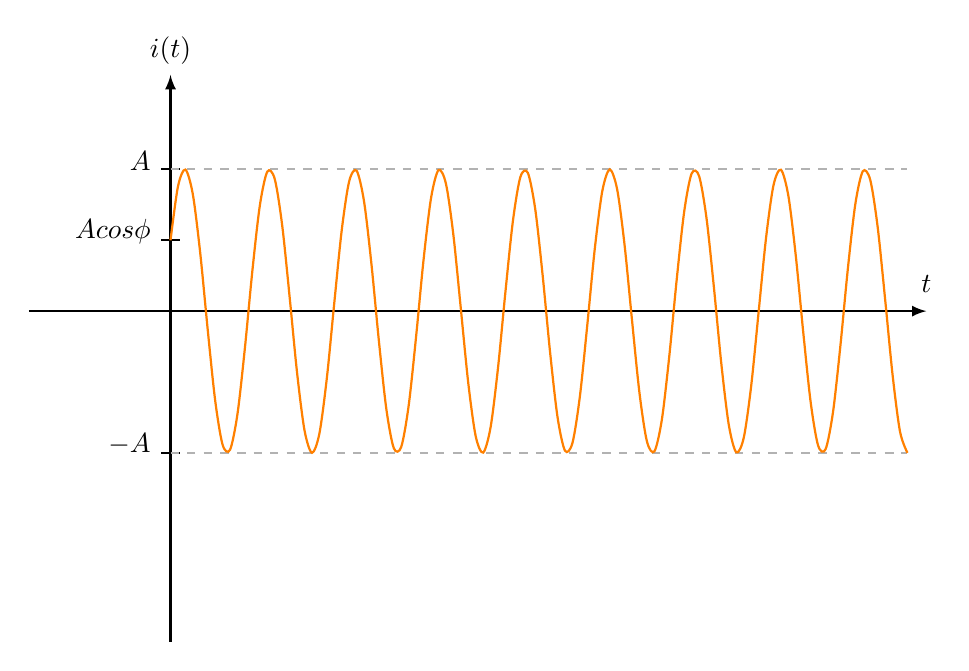
\begin{tikzpicture}[>=latex, thick, scale=1.2]
			% Definizioni per personalizzare il grafico
			\def\A{1.5}
			\def\Phi{-60}
			\def\omega{400}
			
			% --- Assi ---
			% Asse orizzontale (Tempo t)
			\draw[->] (-1.5, 0) -- (8, 0) node[right, above = 3 pt] {$t$};
			% Asse verticale (Corrente i_L(t))
			\draw[->] (0, -3.5) -- (0, 2.5) node[above] {$i(t)$};
			
			% --- Etichette ---
			
			\draw (0.1, {\A * cos(\Phi)}) -- (-0.1, {\A * cos(\Phi)}) node[above=3pt,left] {$Acos\phi$};
			\draw (0.1, {\A}) -- (-0.1,{\A}) node[above=3pt,left] {$A$};
			\draw (0.1, {-\A}) -- (-0.1,{-\A}) node[above=3pt,left] {$-A$};
			
			% --- Curva ---
			
			\draw[black!30,  thick, domain=0:7.8, samples=100, dashed] 
			plot (\x, {\A});
			\draw[black!30,  thick, domain=0:7.8, samples=100, dashed] 
			plot (\x, {-\A});
			\draw[orange,  thick, domain=0:7.8, samples=100, smooth] 
			plot (\x, {\A * cos(\omega *\x + \Phi)});
		\end{tikzpicture}
		\label{fig:nonsmorzata}
		\caption{}
	\end{figure}
\end{enumerate}
Per ricapitolare, osserviamo gli andamenti delle quattro risposte a confronto in \cref{fig:rlcslriassunto}, ottenute mantenendo la stessa $\omega_0$ e facendo variare $\alpha$ come descritto nella legenda.
Osserviamo in particolare la differente altezza dei picchi, e il fatto che la risposta sottosmorzata è quella che porta all'assestamento più velocemente\footnote{Per quanto alla nota precedente, in questo caso la risposta sottosmorzata entra più rapidamente in una generica fascia di tolleranza arbitraria, valutabile visivamente, in quanto si è selezionato un valore di $\zeta = 0.85$, adatto a mostrare il decadimento iniziale rapido, anche se questo non mostra la natura oscillatoria della risposta}
\begin{figure}
	\centering
	\includegraphics[width=0.9\linewidth]{rlcriassunto}
	\caption{}
	\label{fig:rlcslriassunto}
\end{figure}


\subsubsection{RLC serie - Evoluzione forzata}
Facciamo riferimento a \cref{fig:rlcsf}, con regime stazionario con interruttore aperto per $t=0^-$, chiusura dell'interruttore per $t=0$, transitorio per $t\geq 0$
\begin{figure}[H]
	\centering
	\includegraphics[width=0.7\linewidth]{rlcsf}
	\caption{}
	\label{fig:rlcsf}
\end{figure}
Con calcoli analoghi a quelli svolti nel caso dell'evoluzione libera,
\[LKT:\ v_R(t) + v_L(t) + v_C(t) = V_g\]
Utilizzando le leggi costitutive e notando che la corrente che attraversa i tre componenti, collegati in seri, è la stessa $i(t) = i_C(t) = C\frac{dv_C}{dt}$,
\[RC\frac{dv_C}{dt} + LC\frac{d^2i}{dt^2} + v_C(t)= V_g\]
\begin{equation}\label{eq:rlc1}
	\frac{d^2v_C}{dt^2} + \frac{R}{L}\frac{dv}{dt} + \frac{1}{LC} v_c(t) = V_g
\end{equation}
Notiamo quindi che la forma è la stessa dell'\cref{eq:rlc}, in cui però l'incognita è $v_C(t)$ anziché $i(t)$, e l'\cref{eq:rlc1} non è omogenea.
Sfruttiamo la linearità del circuito, quindi scomponiamo la risposta completa in una risposta transitoria $v_{C,t} (t)$ e una a regime $v_{C,r}$:
\[v_C(t) = v_{C,t}(t) + v_{C,r}\]
Per la risposta transitoria,
\[\frac{d^2v_C}{dt^2} + \frac{R}{L}\frac{dv}{dt} + \frac{1}{LC}v_c(t) = 0\]
che è esattamente identica nella forma all'\cref{eq:rlc}.
Dunque, in base alla presenza dei componenti R, L, C, il circuito può avere una risposta transitoria di uno dei quattro tipi già descritti sopra.
\begin{enumerate}
	\item $\Delta > 0$ (\textit{Risposta sovrasmorzata});
	\item $\Delta = 0$ (\textit{Risposta smorzata critica});
	\item $\Delta < 0$ con $\alpha > 0$ (\textit{Risposta sottosmorzata});
	\item $\Delta < 0$ con $\alpha = 0$ (\textit{Risposta senza smorzamento}).
\end{enumerate}

Rimangono da determinare soltanto i parametri $A_1,\ A_2$, dipendenti dalle condizioni iniziali:
\begin{enumerate}
	\item $v_C(0^+) = v_C (0^-) = V_0$
	\item $\left. \frac{dv_C}{dt} \right |_{0^+}$, la quale deve essere ricavata dallo studio del circuito a $t = 0^+$, similmente a quanto fatto per la corrente nel circuito in evoluzione libera. Sostituiamo dunque il condensatore con un generatore di tensione $V_0$ e l'induttore con un generatore di corrente $I_0$. Dal circuito così ottenuto è poi possibile determinare il valore di $\left. \frac{dv_C}{dt} \right |_{0^+}$ sfruttando il fatto che $\frac{dv_c}{dt} = Ci_C$.
\end{enumerate}
Per determinare la risposta a regime, è sufficiente, poi, effettuare un'analisi del circuito in regime stazionario a $t=\infty$, considerando che gli induttori sono equivalenti a cortocircuiti e i condensatori a rami aperti (\cref{fig:rlcsf1}).
\begin{figure}[H]
	\centering
	\includegraphics[width=0.7\linewidth]{rlcsf1}
	\caption{}
	\label{fig:rlcsf1}
\end{figure}
\[LKT: v_C(\infty) = V_g - v_R(\infty) = V_g + Ri_R = V_g\]
Osserviamo nel grafico in \cref{fig:rlcsfriassunto} l'andamento della risposta completa nel tempo in base a diversi valori della resistenza, dunque di $\alpha$ del circuito.
\begin{figure}[H]
	\centering
	\includegraphics[width=0.9\linewidth]{rlcsfriassunto}
	\caption{}
	\label{fig:rlcsfriassunto}
\end{figure}
Siccome la forma delle soluzioni alle equazioni differenziali è la stessa per tutti i circuiti, nella risoluzione degli esercizi è soltanto necessario determinare i valori iniziali e finali (tramite l'analisi a \textit{istanti strategici}) per ottenere la soluzione specifica. Gli esercizi proposto sono dunque studi semplificati di transitori.
\begin{ex}[Studio semplificato di un transitorio]
	Si consideri il circuito in \cref{fig:exrlc}
	\begin{figure}[H]
		\centering
		\begin{circuitikz}
		
		% Definisci le coordinate dei nodi principali
		\coordinate (A) at (0, 0);     % Angolo in basso a sinistra
		\coordinate (D) at (0, 3);     % Angolo in alto a sinistra
		\coordinate (C_split) at (4, 3);   % Punto di diramazione superiore (per R2/Switch)
		\coordinate (C_end) at (6, 3);     % Punto di diramazione superiore (per C)
		\coordinate (B_split) at (4, 0);   % Punto di diramazione inferiore (per R2/Switch)
		\coordinate (B_end) at (6, 0);     % Punto di diramazione inferiore (per C)
		\coordinate (E) at (4, 1.5);       % Nodo intermedio per R2/switch
		
		% 1. Branca di Sinistra (Generatore)
		\draw (A) to[V, v<=$V_g$] (D);
		
		% 2. Branca Superiore (R1 e L)
		\draw (D) to[R, l_=$R_1$] (2, 3)
		to[L, l=$L$] (C_split); 
		
		% 3. Linea superiore di collegamento
		\draw (C_split) -- (C_end);
		
		% 4. Branca Centrale (R2 e Interruttore)
		
		% Resistenza R2
		\draw (C_split) to[R, l_=$R_2$, -*] (E);
		
		% INTERRUTTORE COMPATIBILE: Usiamo 'switch'
		\draw (E) to [switch, l_={$t=0$}] (B_split); 
		
		% Aggiungi l'etichetta della corrente manualmente (per compatibilità)
		\node at (4.5, 0.75) {$i(t)$};
		
		% Aggiungi la freccia per l'azione di chiusura del circuito (come nel disegno a mano)
		%\draw[->] (3.8, 1.2) arc (270:315:0.5); 
		
		% 5. Branca di Destra (C) - ORA SEPARATA
		\draw (C_end) to[C, l=$C$] (B_end); 
		
		% 6. Linea inferiore di collegamento (chiusura del circuito)
		\draw (B_split) -- (A);
		\draw (B_split) -- (B_end); % Collega le basi dei rami paralleli
		\end{circuitikz}
		\caption{}
		\label{fig:exrlc}
	\end{figure}
	
	Si determinino: $i_L(0^-)$,$i_C(0^-)$, $\left. \frac{di_L}{dt}\right|_{0^+}$, $\left. \frac{dv_c}{dt}\right|_{0^+}$, $E_L (\infty)$, $E_L (\infty)$.
	Iniziamo studiando il circuito a $t= 0^-$, con interruttore chiuso, in regime stazionario. Il circuito si semplifica come in \cref{fig:exrlc1}
	\begin{figure}[H]
		\centering
		\begin{circuitikz}
		% --- Coordinate ---
		\coordinate (A) at (0,0);     % Massa sinistra
		\coordinate (B) at (0,3);     % Alto sinistra
		\coordinate (C) at (3,3);     % Nodo dopo R1
		\coordinate (D) at (5,3);     % Nodo sopra R2
		\coordinate (E) at (5,0);     % Nodo sotto R2
		\coordinate (F) at (7,3);     % Terminale aperto alto
		\coordinate (G) at (7,0);     % Terminale aperto basso
		
		% --- 1. Generatore e R1 ---
		\draw (A) to[V, l=$V_g$] (B);
		\draw (B) to[R, l=$R_1$] (C);
		
		% --- 2. Induttore (come Corto Circuito) ---
		% Disegno un filo (short) con due pallini (*-*) per evidenziare che lì c'era L
		\draw (C) to[short, *-*, i=$i_L$] (D);
		% NOTA: Se "i=$i_L$" ti da errore, cancellalo e usa la riga sotto:
		% \node at (4, 3.5) {$i_L \rightarrow$};
		
		% --- 3. Ramo Centrale (R2) ---
		% Uso v=... per la tensione. Se da errore, usa i nodi manuali.
		\draw (D) to[R, l=$R_2$, v=$v_{R2}$] (E);
		
		% --- 4. Ramo di Destra (Condensatore come Circuito Aperto) ---
		\draw (D) -- (F); % Filo superiore
		\draw (E) -- (G); % Filo inferiore
		
		% "open" crea uno spazio vuoto, "o-o" mette i cerchietti dei terminali
		\draw (F) to[open, v=$v_C$, o-o] (G);
		
		% --- 5. Chiusura del circuito (massa) ---
		\draw (E) -- (A);
		
		\end{circuitikz}
		\caption{}
		\label{fig:exrlc1}
	\end{figure}
	\[i_L(0^-) = \frac{V_g}{R_1 + R_2}\]
	\[v_C(0^-) = R_2 i_{R_2} = R_2 \frac{V_g}{R_1 + R_2}\]
	Studiamo il circuito a $t = 0^+$. Per le proprietà di continuità, analogamente a quanto osservato nella teoria precedente, possiamo considerare i componenti dinamici come generatori indipendenti, mantenendo i VDR scelti in precedenza (\cref{fig:exrlc2}).
	
	\begin{figure}[H]
		\centering
		\begin{circuitikz}
			
			% --- Coordinate ---
			\coordinate (A) at (0,0);
			\coordinate (D) at (0,4);
			\coordinate (NodeL) at (4,4);    % Nodo sopra R2
			\coordinate (NodeR) at (8,4);    % Nodo sopra Generatore equiv C
			\coordinate (GndL) at (4,0);     % Nodo sotto R2
			\coordinate (GndR) at (8,0);     % Nodo sotto Generatore equiv C
			
			% --- 1. Generatore Vg (Sinistra) ---
			\draw (A) to[V, l=$V_g$] (D);
			
			% --- 2. Ramo Superiore: R1 e Generatore di Corrente (ex Induttore) ---
			% Nota: I generatori di corrente si indicano con 'isource' (o 'I' nelle vecchie versioni)
			\draw (D) to[R, l=$R_1$] (2,4)
			to[isource, l=$\frac{V_g}{R_1+R_2}$] (NodeL);
			
			% --- 3. Ramo Centrale: R2 e Interruttore Aperto ---
			% Disegno l'interruttore esplicitamente aperto per chiarezza
			\draw (NodeL) to[R, l=$R_2$] (4,2.5);
			\draw (4,2.5) to[open, o-o] (4,1.5); % Spazio vuoto con terminali (switch aperto)
			\draw (4,1.5) -- (GndL);
			
			% --- 4. Ramo Destro: Generatore di Tensione (ex Condensatore) ---
			\draw (NodeL) -- (NodeR);
			
			% Uso 'V' per il generatore che sostituisce C.
			% \displaystyle serve a rendere la frazione leggibile e grande
			\draw (NodeR) to[V, l=$R_2 \frac{V_g}{R_1+R_2}$] (GndR);
			
			\draw (GndR) -- (GndL) -- (A);
		\end{circuitikz}
		\caption{}
		\label{fig:exrlc2}
	\end{figure}
	\[\left. \frac{dv_c}{dt} \right |_{0^+} = \frac{i_C}{C} = \frac{i_L}{C} = \frac{1}{C}\frac{V_g}{R_1 + R_2}\ (V\cdot s^{-1})\]
	\[\left. \frac{di_L}{dt} \right |_{0^+} = \frac{v_L}{L} = \frac{ V_g - v_R - v_C}{L} = \frac{V_g}{L} \left( 1 - \frac{R_1}{R_1 + R_2} -\frac{R_2}{R_1 + R_2} \right) = 0\]
	Studiamo il circuito a $t = \infty$ (\cref{fig:exrlc3}).
	\begin{figure}[H]
		\centering
		\begin{circuitikz}% Aumento leggermente la scala per chiarezza
			
			% Definizione delle coordinate principali per facilitare il disegno
			\coordinate (A_bot) at (0,0); % Angolo in basso a sinistra
			\coordinate (A_top) at (0,3); % Angolo in alto a sinistra
			\coordinate (B_top) at (4,3); % Nodo di giunzione superiore centrale
			\coordinate (B_mid) at (4,1.5); % Punto intermedio nel ramo centrale
			\coordinate (B_bot) at (4,0); % Nodo di giunzione inferiore centrale
			\coordinate (C_top) at (7,3); % Angolo in alto a destra
			\coordinate (C_bot) at (7,0); % Angolo in basso a destra
			
			% --- Ramo di Sinistra e Superiore (Generatore, R1, L) ---
			% Disegno dal basso a sinistra, salgo col generatore, poi a destra con R1 e L
			\draw (A_bot) to[V, l=$V_g$] (A_top)
			to[R, l=$R_1$] (2,3) % Punto intermedio per spaziare R1 e L
			to[L, l=$L$] (B_top);
			
			% --- Ramo Centrale (R2 e Interruttore) ---
			% Parto dal nodo superiore centrale (B_top) e scendo.
			% Uso '*-' per mettere il pallino di giunzione all'inizio.
			\draw (B_top) to[R, l=$R_2$, *-] (B_mid)
			% 'opening switch' disegna la freccia di apertura.
			% Aggiungo l'etichetta t=0.
			to[nos, l={$t=\infty$}] (B_bot);
			
			% --- Ramo di Destra (Condensatore) ---
			% Continuo il filo superiore da B_top a C_top, poi scendo col condensatore.
			\draw (B_top) -- (C_top)
			to[C, l=$C$] (C_bot);
			
			% --- Chiusura del circuito inferiore ---
			% Collego i punti inferiori per chiudere la massa.
			% Uso '-*' per aggiungere il pallino di giunzione sotto l'interruttore.
			\draw (C_bot) -- (B_bot) to[short, -*] (A_bot);
		\end{circuitikz}
		\caption{}
		\label{fig:exrlc3}
	\end{figure}
	
	\[E_L(\infty) = \frac{1}{2}Li_L^2(\infty) = \frac{1}{2}L\left(\frac{V_g}{R_1}\right)^2 \]
	\[E_C(\infty) = \frac{1}{2}Cv_C^2(\infty) = \frac{1}{2}C(Ri_{R_2}(\infty))^2 = 0 \]
\end{ex}
\subsubsection{RLC parallelo - Evoluzione forzata}
Analizziamo un circuito RLC parallelo, direttamente in evoluzione forzata. Da questa trattazione, poi, è possibile ricavare come caso particolare l'evoluzione libera.
Consideriamo, ad esempio, un circuito come in \cref{fig:rlcp}, che rappresenta il caso realistico in cui il transitorio è innescato dalla chiusura di un interruttore. Altri scenari possibili potrebbero essere più complicati.
\begin{figure}[H]
	\centering
	\begin{circuitikz}
		% --- Definisco le coordinate per chiarezza ---
		\coordinate (A_bot) at (0,0);  % Basso Sinistra
		\coordinate (A_top) at (0,3);  % Alto Sinistra (sopra Ig)
		\coordinate (B_top) at (3,3);  % Nodo sopra R
		\coordinate (B_bot) at (3,0);  % Nodo sotto R
		\coordinate (C_top) at (6,3);  % Nodo sopra L
		\coordinate (C_bot) at (6,0);  % Nodo sotto L
		\coordinate (D_top) at (8,3);  % Nodo sopra C
		\coordinate (D_bot) at (8,0);  % Nodo sotto C
		
		% --- Parte Sinistra: Generatore Ig e Resistenza R ---
		% Disegno il generatore di corrente (I) che sale
		\draw (A_bot) to[I, l=$I_g$] (A_top);
		
		% Collega la parte superiore e disegna la resistenza R
		\draw (A_top) -- (B_top)
		to[R, l=$R$, *-*] (B_bot) % *-* mette i pallini ai nodi
		-- (A_bot); % Chiude il loop in basso
		
		% --- Parte Centrale: Interruttore ---
		% 'closing switch' disegna l'interruttore aperto con la freccia che chiude
		\draw (B_top) to[closing switch] (C_top);
		
		% --- Parte Destra: Induttore L e Condensatore C ---
		% Disegno l'induttore L
		\draw (C_top) to[L, l=$L$, *-*] (C_bot);
		
		% Collega il condensatore C in parallelo
		\draw (C_top) -- (D_top)
		to[C, l=$C$] (D_bot)
		-- (C_bot);
		
		% --- Collegamento di massa inferiore ---
		% Unisce la massa di sinistra con quella di destra
		\draw (B_bot) -- (C_bot);
	\end{circuitikz}
	\caption{}
	\label{fig:rlcp}
\end{figure}
Applichiamo lo stesso metodo già utilizzato per RLC serie per indagare il comportamento del circuito per $t \geq 0$, durante il transitorio.

\[LKC:\ i_R(t) + i_L(t) + i_C(t) = I_g\]
\[\frac{v(t)}{R} + i_L(t) + C\frac{dv}{dt} = I_g\]
\[\frac{L}{R} \frac{di_L}{dt} + i_L(t) + C\frac{d^2i_L}{dt} = I_g\]

\begin{equation} \label{eq:rlcp}
	\frac{d^2i_L}{dt} + \frac{1}{RC} \frac{di_L}{dt} + \frac{1}{LC} i_L(t) = \frac{1}{LC}I_g
\end{equation}
Notiamo che l'\cref{eq:rlcp} è molto simile all'\cref{eq:rlc1}, con l'unica differenza che in questo caso è la tensione la funzione incognita. In questo caso, $\omega_0$ ha lo stesso valore in funzione dei parametri del sistema ($\omega_0 = \frac{1}{\sqrt{LC}}$), mentre $\alpha = \frac{1}{2RC}$.
Dunque anche in questo caso il polinomio caratteristico è 
\[\lambda^2 + 2 \alpha \lambda + \omega_0^2 = 0\]
\[\lambda_{1,2} = -\alpha \pm \sqrt{\Delta},\quad \Delta = \alpha^2 - \omega_0^2\]
Siccome il circuito è lineare, possiamo leggere la risposta completa come somma di una risposta transitoria e una regime:
\[i_L(t) = i_{L,t} (t) + i_{L,R}\]
La risposta transitoria può avere le forme già descritte sopra:
\begin{enumerate}
	\item $\Delta > 0$, \textit{Risposta sovrasmorzata};
	\item $\Delta = 0$, \textit{Risposta smorzata critica};
	\item $\Delta < 0$ con $\alpha > 0$, \textit{Risposta sottosmorzata};
	\item $\Delta < 0$ con $\alpha = 0$, \textit{Risposta senza smorzamento}.
\end{enumerate}
I parametri $A_1,\ A_2$ dipendono dalle condizioni iniziali, $i_L(0^+) = i_L(0^-)$; $\left. \frac{di_L}{dt} \right |_{0^+}$, che può essere ottenuta analizzando il circuito all'istante iniziale, considerando i componenti dinamici come generatori indipendenti per quell'istante, in modo del tutto analogo a quanto sopra.\\
Per determinare la risposta a regime, consideriamo il circuito per $t = \infty$, a transitorio concluso (\cref{fig:rlcp1}). Dunque, banalmente,
\[i_{L,R} = I_g\]
\begin{figure}[H]
	\centering
	\begin{circuitikz}[american]
		% Coordinate
		\coordinate (A_bot) at (0,0);
		\coordinate (A_top) at (0,3);
		\coordinate (B_top) at (3,3);
		\coordinate (B_bot) at (3,0);
		\coordinate (C_top) at (6,3);
		\coordinate (C_bot) at (6,0);
		\coordinate (D_top) at (9,3);
		\coordinate (D_bot) at (9,0);
		
		% 1. Generatore di Corrente Ig
		\draw (A_bot) to[I, l=$I_g$] (A_top);
		
		% 2. Resistenza R (che viene cortocircuitata)
		% Aggiungo i_R verso il basso
		\draw (A_top) -- (B_top);
		\draw (B_top) to[R, l=$R$, i>=$i_R$] (B_bot);
		
		% (Opzionale) Se vuoi disegnare la barra trasversale che indica che è esclusa:
		%\draw[thick] (2.5, 0.5) -- (3.5, 2.5); 
		
		% 3. Induttore -> Corto Circuito (Filo)
		% Uso *-* per mostrare i nodi pieni come nel disegno
		\draw (B_top) -- (C_top);
		\draw (C_top) to[short, *-*, v=$v_L{=}0$] (C_bot);
		
		% 4. Condensatore -> Circuito Aperto
		% Uso o-o per i terminali aperti
		\draw (C_top) -- (D_top);
		\draw (D_top) to[open, o-o, v=$v_C$, i=$i_C{=}0$] (D_bot);
		
		% Collegamenti inferiori (Massa)
		\draw (A_bot) -- (D_bot);
	\end{circuitikz}
	\caption{}
	\label{fig:rlcp1}
\end{figure}
Perciò, gli andamenti possibili per la risposta $i_L(t) = i_{L,t}(t) + I_g$ sono rappresentati in \cref{fig:rlcp2}.
\begin{figure}[H]
	\centering
	\includegraphics[width=0.8\linewidth]{rlcp2}
	\caption{}
	\label{fig:rlcp2}
\end{figure}
Nel grafico, generato per opportuni valori delle condizioni iniziali adatti a mostrare la stretta analogia, notiamo, come previsto la totale somiglianza degli andamenti con quelli graficati in \cref{fig:rlcsfriassunto}.\\
Omettiamo per semplicità lo studio delle altre variabili del circuito, che possono essere semplicemente determinati tramite le leggi di Kirchhoff.

\subsection{Calcolo delle costanti $A_1$ e $A_2$}
Il calcolo è analogo per tutti i casi. Prendendo, ad esempio, il caso della risposta sovrasmorzata, esse possono essere ricavate dal seguente sistema di due equazioni in due incognite, dove i valori di $x(t)$ e della sua derivata possono essere determinati per ispezione diretta, come mostrato sopra.
\[\begin{cases}
	x(t) = A_1 e^{\lambda_1 t} + A_2 e^{\lambda_2 t}\\
	\frac{dx}{dt} = \lambda_1 A_1 e^{\lambda_1 t} + \lambda_2 A_2 e^{\lambda_2 t}
\end{cases}\]
Per semplificare i calcoli, siccome $A_1$ e $A_2$ sono costanti, possiamo studiare il sistema per $t=0^+$, e usare i necessari valori dall'ispezione del circuito, come anticipato sopra:
\[\begin{cases}
	x(0^+) = A_1 + A_2 \\
	\left. \frac{dx}{dt} \right |_{0^+} = \lambda_1 A_1 + \lambda_2 A_2
\end{cases}\]
\[\begin{cases}
	A_1 = x(0^+) - A_2\\
	\left. \frac{dx}{dt} \right |_{0^+} = \lambda_1 x(0^+) - \lambda_1 A_2 + \lambda_2 A_2 = \lambda_1 x(0^+) + A_2 (\lambda_2 \lambda_1)
\end{cases}\]
\[\begin{cases}
	A_1 = \frac{\left. \frac{dx}{dt} \right |_{0^+} - \lambda_2 x(0^+)}{\lambda_1 - \lambda_2}
	A_2 = \frac{\left. \frac{dx}{dt} \right |_{0^+} - \lambda_1 x(0^+)}{\lambda_2 - \lambda_1}\\
\end{cases}\]
Per le altre forme, si ottengono forme analoghe (non identiche, in quanto la forma di partenza è differente).

\subsection{Risonanza}
\subsubsection{Risonanza - RLC serie}
Esploriamo in questa sezione il concetto di \textit{risonanza} in un circuito RLC.\\
Consideriamo un ramo di un circuito RLC serie in regime sinusoidale, come in \cref{fig:risonanza}, e indaghiamone il comportamento al variare della frequenza $\omega$ di oscillazione della tensione nel circuito.

\begin{figure}[H]
	\centering
	\begin{circuitikz}[american]
		% Coordinate
		\coordinate (In_Bot) at (0,0);
		\coordinate (In_Top) at (0,3);
		\coordinate (Top_Right) at (4,3);
		\coordinate (Bot_Right) at (4,0);
		
		% --- MODIFICA QUI ---
		% Disegno da SOPRA a SOTTO per avere il + in alto.
		% Uso '<' per girare la freccia verso l'alto.
		% Uso '^' (opzionale) per spostare l'etichetta se si sovrappone
		\draw (In_Top) to[open, v^>=$\underline{V}$, o-o] (In_Bot);
		% --------------------
		
		% Ramo Superiore
		\draw (In_Top) to[short, i=$\underline{I}$] (1,3) 
		to[generic, l=$\underline{Z}_R$] (Top_Right);
		
		% Ramo Destro
		\draw (Top_Right) to[generic, l=$\underline{Z}_L$] (Bot_Right);
		
		% Ramo Inferiore
		\draw (Bot_Right) to[generic, l=$\underline{Z}_C$] (In_Bot);
		
	\end{circuitikz}
	\caption{}
	\label{fig:risonanza}
\end{figure}

\[\underline{Z} = Z_R + \underline{Z_L} + \underline{Z_C} = R + j \omega L - \frac{j}{\omega C} = R + jX\]
\[X(\omega) = \omega L - \frac{1}{\omega C}\]
Notiamo che la reattanza del sistema, all'aumentare della frequenza, ha un termine che aumenta e uno che diminuisce. Ci chiediamo dunque se esista un valore $\omega_0$ tale da annullare la reattanza:
\[\omega_0 L - \frac{1}{\omega_0 C} \Leftrightarrow \omega_0 = \frac{1}{\sqrt{LC}}\]
Notiamo che questo valore è proprio quello che abbiamo impiegato come \textit{frequenza di risonanza} nella descrizione dei transitori. Questa è l'origine del termine: per $\omega = \omega_0$, il circuito si dice operante in condizione di risonanza, e
\[\underline{Z} = R + j0 = R\]
L'interesse per questo circuito è legato alle proprietà dell'andamento della corrente che scorre nel circuito al variare della frequenza.\\
\begin{center}
	% 2. Aumenta l'altezza delle righe (2 volte il normale)
	\renewcommand{\arraystretch}{2.5}
	
	% 3. Aumenta lo spazio laterale nelle celle (padding orizzontale)
	\setlength{\tabcolsep}{25pt}
	\begin{tabular}{c|c|c}
		
		\textbf{$\omega$} &\textbf{$X$} & \textbf{$\displaystyle \underline{I}=\frac{\underline{V}}{\sqrt{R^2 + X^2}}$}\\ % Intestazione della tabella in modalità matematica
		\hline % Linea orizzontale sotto l'intestazione
		$0$ & $\displaystyle \lim_{\omega \to 0} \left( \omega L - \frac{1}{\omega C} \right) = 0 - \infty = -\infty$ & $0$ \\ % Contenuto della riga con formula complessa
		
		$\omega_0$ & $0$ & $\frac{V}{R}$\\
		 
		$\infty$ & $\infty$ & $0$\\
	\end{tabular}\\
\end{center}
Ci aspettiamo dunque un andamento della corrente che esibisca un picco alla frequenza di risonanza e tenda a 0 a $\omega = \pm \infty$. Tale picco sarà più alto tanto più piccola la resistenza. Per una resistenza nulla, si avrebbe un comportamento asintotico: se non opportunamente limitato, la corrente tenderà all'infinito (\cref{fig:risonanza1}). All'atto pratico, salirà fino al limite di protezione del generatore utilizzato, imposto dai produttori per evitare danni irreversibili ai circuiti interni e collegati.\\
\begin{figure}[H]
	\centering
	\includegraphics[width=0.7\linewidth]{risonanza1}
	\caption{}
	\label{fig:risonanza1}
\end{figure}

Analizziamo anche l'andamento di $\varphi = \varphi(\omega) = arg(\underline{Z})$.\\
\begin{center}
	\renewcommand{\arraystretch}{2.5}
	
	% 3. Aumenta lo spazio laterale nelle celle (padding orizzontale)
	\setlength{\tabcolsep}{25pt}
	\begin{tabular}{c|c}
		\textbf{$\omega$} & \textbf{$\varphi = arg(\underline{Z}) = atan(\frac{X}{R})$}\\ % Intestazione della tabella in modalità matematica
		\hline % Linea orizzontale sotto l'intestazione
		$0$ & $atan{-\infty} = -\frac{\pi}{2}$\\ % Contenuto della riga con formula complessa
		
		$\omega_0$ & $atan(0) = 0$\\
		 
		$\infty$ & $atan{\infty} = \frac{\pi}{2}$
	\end{tabular}\\
\end{center}


Notiamo dunque che lo sfasamento dovrà avere un andamento analogo a quello della funzione arcotangente, con radice in $\omega_0$. A basse frequenze ($\omega < \omega_0$), il circuito è dominato dal comportamento capacitivo; al contrario, alle alte frequenze ($\omega > \omega_0$), dal comportamento induttivo. Per $\omega 0 \omega_0$, il comportamento è ohmico, puramente resistivo, con corrente e tensione in fase (\cref{fig:risonanza2}). Questo deve essere tenuto in considerazione per ottenere il comportamento desiderato da induttori e capacitori in regime sinusoidale.
\begin{figure}[H]
	\centering
	\includegraphics[width=0.7\linewidth]{risonanza2}
	\caption{}
	\label{fig:risonanza2}
\end{figure}

\subsubsection{Antirisonanza - RLC parallelo}
\begin{figure}[H]
	\centering
	\begin{circuitikz}[american]
		% Coordinate
		\coordinate (In_Top) at (0,3);
		\coordinate (In_Bot) at (0,0);
		\coordinate (Node_Top) at (3,3); % Nodo sopra il parallelo
		\coordinate (Node_Bot) at (3,0); % Nodo sotto il parallelo
		\coordinate (Par_Right_Top) at (5,3);
		\coordinate (Par_Right_Bot) at (5,0);
		
		% 1. Tensione V (+ sopra, - sotto, freccia in su)
		% Disegno da SOPRA (In_Top) a SOTTO (In_Bot) -> Il '+' va alla partenza (sopra).
		% Uso '<=' per invertire la freccia (farla puntare verso l'alto).
		\draw (In_Top) to[open, v<=$\underline{V}$, o-o] (In_Bot);
		
		% 2. Ramo Serie: Corrente I e Resistenza R
		% Uso un piccolo tratto 'short' per la corrente, poi la Resistenza
		\draw (In_Top) to[short, i=$\underline{I}$] (1,3) 
		to[R, l=$R$] (Node_Top);
		
		% 3. Parallelo - Ramo Sinistro (Simbolo C, Label L)
		% Nota: Nel tuo disegno questo componente ha il simbolo del condensatore (C)
		% ma l'etichetta 'L'. Ho rispettato il disegno.
		\draw (Node_Top) to[C, l=$L$] (Node_Bot);
		
		% 4. Parallelo - Ramo Destro (Simbolo L, Label C)
		% Collega a destra, scende con l'induttore, torna a sinistra
		\draw (Node_Top) -- (Par_Right_Top)
		to[L, l=$C$] (Par_Right_Bot)
		-- (Node_Bot);
		
		% 5. Chiusura del circuito (linea di fondo)
		\draw (Node_Bot) -- (In_Bot);
		
	\end{circuitikz}
	\caption{}
	\label{fig:risonanza3}
\end{figure}
Consideriamo il circuito in \cref{fig:risonanza3}, e proseguiamo con considerazioni analoghe.
\[\underline{Z} = R + jX = \frac{j\omega L \cdot (-\frac{j}{\omega C})}{j\omega L - \frac{j}{\omega C}} = - j \frac{\frac{L}{C}}{\omega L - \frac{1}{\omega C}} \]
Dunque, 
\[X(\omega) = - \frac{\frac{L}{C}}{\omega L - \frac{1}{\omega C}} \] 
Osserviamo che non esiste alcun valore di $omega$ che annulla la reattanza. Osserviamo, anzi, che la reattanza tende a infinito per $omega = \omega_0$:
\[X(\omega_0) = -\frac{\frac{L}{C}}{0}\]
\begin{center}
	% 2. Aumenta l'altezza delle righe (2 volte il normale)
	\renewcommand{\arraystretch}{2.5}
	
	% 3. Aumenta lo spazio laterale nelle celle (padding orizzontale)
	\setlength{\tabcolsep}{25pt}
	\begin{tabular}{c|c}
		
		\textbf{$\omega$} & \textbf{$X$}\\ % Intestazione della tabella in modalità matematica
		\hline % Linea orizzontale sotto l'intestazione
		$0$ & $0$ \\ % Contenuto della riga con formula complessa
		
		$\omega_0^-$ & $\infty$\\
		
		$\omega_0^+$ & $- \infty$\\
		
		$\infty$ & $0$\\
	\end{tabular}\\
\end{center}
L'andamento della reattanza è quindi quello rappresentato in \cref{fig:risonanza4}, che ha comportamento duale a quello della risonanza: si ha comportamento ohmico-induttivo per basse frequenze e ohmico-capacitivo ad alte frequenze. Le correnti tendono ad annullarsi in prossimità della pulsazione di antirisonanza.\\
\begin{figure}[H]
	\centering
	\includegraphics[width=0.7\linewidth]{risonanza4}
	\caption{}
	\label{fig:risonanza4}
\end{figure}
Notiamo che per $\omega = 0$, il parallelo RC è visto come un cortocircuito, con $\underline{Z_L} = 0$ e $\underline{Z_C} = \infty$ e tutta la corrente scorre sull'induttore, che si comporta come un circuito aperto, mentre il condensatore come un cortocircuito.\\
Per $\omega = \infty$, il comportamento è perfettamente speculare, con il condensatore che si comporta come cortocircuito e l'induttore come circuito aperto.\\
Per $\omega = \omega_0$, nessuno dei due componenti ha impedenza infinita o nulla, tuttavia il parallelo dei due ha impedenza infinita, e perciò la corrente entrante e uscente dal parallelo è nulla. I due componenti singolarmente sentono la tensione V applicata ai capi del ramo (la caduta sul resistore è nulla perché non scorre corrente). Perciò su essi, nel ramo interno al parallelo in realtà si ha una corrente, e per la LKC $\underline{I_C} = \underline{I_L} = j\underline{V} \omega C = -\frac{j \underline{V}}{\omega L}$, detta \textit{corrente di circolazione}. In fase di progettazione, è dunque necessario verificare che anche questa corrente sia compatibile con le caratteristiche dei componenti, e non rischi di danneggiarli.

\section{Validità dei circuiti a parametri concentrati}
Ricordiamo che le Leggi di Kirchhoff derivano dall'ipotesi di completo isolamento dei componenti, cioè dall'assenza di variazione di campo di induzione magnetica e di campo elettrico al di fuori dei componenti circuitali.

\[\nabla \times \vec E = -\frac{\partial \vec B}{\partial t} \longrightarrow \frac{\partial \vec B}{\partial t}\approx 0 \Longrightarrow \nabla \times \vec E = 0 \Longrightarrow LKT\]

\[\nabla \times \vec H = \vec J + \frac{\partial \vec D}{\partial t} \longrightarrow \frac{\partial \vec D}{\partial t}\approx 0 \Longrightarrow \nabla \times \vec H = \vec J \Longrightarrow LKC\]

In DC le due condizioni sopra indicate sono sempre vere: il regime è stazionario dunque $\frac{d}{dt} = 0$. In AC e in transitorio, tanto più alta è la frequenza di oscillazione tanto maggiori sono i valori delle derivate, perciò è legittimo porsi il problema di quale sia la frequenza per la quale il modello a parametri concentrati è completamente inefficace, e dà dunque predizioni inaccurate. Procediamo dunque a studiare un criterio veloce, per quanto rudimentale, per determinare quantitativamente il limite dell'applicazione del modello a parametri concentrati a specifici circuiti.

\subsection{Criterio del tempo di transito}
Consideriamo un frequenza $f$ caratteristica del circuito in analisi. Per un transitorio non si può considerare una frequenza unica, tuttavia in prima approssimazione il ragionamento può essere analogo. Per il circuito in analisi, vale dunque che il periodo è $T = \frac{1}{f}$.\\
Detti $\tau_P$ \textit{ritardo di propagazione}, $d_{max}$ la massima distanza tra due punti del circuito e $c$ la velocità della luce, il modello a parametri concentrati è valido se risulta:
\[T \gg \tau_P = \frac{d_{max}}{c}\]
Se questo è valido, infatti, le variazioni dei campi sono abbastanza lente da permettere di considerare $\vec B$ e $\vec D$ circa costanti nel tempo durante $\tau_P$. 
Osserviamo dunque quali sono le dimensioni massime di un circuito a diverse frequenze comuni per alcune applicazioni. In gran parte delle applicazioni attuali, il modello a parametri concentrati risulta sufficiente per una buona progettazione. Soprattutto su piccola scala, e per elevata precisione, è possibile scontrarsi con i limiti: in tal caso è necessario fare riferimento a teorie più complesse, ripartendo dalle Leggi di Maxwell. In realtà, inoltre, per tali scopi è spesso indispensabile anche tenere conto di fenomeni quantistici.
\begin{center}
	% 2. Aumenta l'altezza delle righe (2 volte il normale)
	\renewcommand{\arraystretch}{2.5}
	
	% 3. Aumenta lo spazio laterale nelle celle (padding orizzontale)
	\setlength{\tabcolsep}{25pt}
	\begin{tabular}{c|c|c}
		
		\textbf{$f$} &\textbf{$T$} & \textbf{$d_max$}\\ % Intestazione della tabella in modalità matematica
		\hline % Linea orizzontale sotto l'intestazione
		$50\ Hz$ & $20\ ms$ & $6000\ km$ \\

		$1\ MHz$ & $1\ \mu s$ & $300\ m$\\
		
		$1\ GHz$ & $1\ ns$ & $0,3\ m$\\
		
		$10\ GHz$ & $100\ ps$ & $3\ cm$\\
	\end{tabular}\\
\end{center}

\end{document}
